\documentclass[12pt,a4paper]{article}
\usepackage[UTF8]{ctex}
\usepackage{graphicx}
\usepackage{geometry}
\usepackage{amsmath}
\usepackage{amsfonts}
\usepackage{amssymb}
\usepackage{listings}
\usepackage{xcolor}
\usepackage{float}
\usepackage{tikz}
\usepackage{fancyhdr}
\usepackage{setspace}
\usepackage{multirow}
\usepackage[most]{tcolorbox}
\tcbset{colback=white,colframe=black,boxrule=0.6pt,arc=0mm,left=3mm,right=3mm,top=2mm,bottom=2mm,breakable,enhanced}
% 下划线填空宏：在水平线上放入左对齐内容
\newcommand{\fillin}[1]{\underline{\makebox[8cm][l]{#1}}}
\usetikzlibrary{shapes,arrows,positioning}

\geometry{left=2.5cm,right=2.5cm,top=3.5cm,bottom=2.5cm}
\setlength{\headheight}{24.64995pt}

% 设置页眉
\pagestyle{fancy}
\fancyhf{}
\fancyhead[C]{\textbf{实验2 简单绘图软件的设计与实现}}
\fancyhead[R]{\thepage}
\renewcommand{\headrulewidth}{2pt}
\renewcommand{\headrule}{\hbox to\headwidth{\leaders\hrule height 2pt\hfill}}

% 设置代码样式
\lstset{
    language=C++,
    basicstyle=\ttfamily\small,
    keywordstyle=\color{blue},
    commentstyle=\color{green!50!black},
    stringstyle=\color{red},
    numbers=left,
    numberstyle=\tiny\color{gray},
    stepnumber=1,
    numbersep=5pt,
    backgroundcolor=\color{gray!10},
    showspaces=false,
    showstringspaces=false,
    showtabs=false,
    frame=single,
    tabsize=2,
    captionpos=b,
    breaklines=true,
    breakatwhitespace=false,
}

\title{\textbf{实验2 简单绘图软件的设计与实现}}
\author{程泽凯 \quad 2023112621}
\date{\today}

\begin{document}

% 自定义封面（按图一）
\begin{titlepage}
    \thispagestyle{empty}
    \begin{spacing}{1.2}
    \centering
    \vspace*{10mm}
    {\zihao{4} 《计算机图形学及人机交互》\par}
    \vspace{20mm}
    {\bfseries\zihao{1} 实 验 报 告\par}
    \vspace{40mm}

    % 基本信息
    \songti\zihao{-3}
    \begin{flushleft}
    \setlength{\tabcolsep}{1em}
    \renewcommand\arraystretch{2}
    \begin{tabular}{@{}ll}
        学\quad 号： & \fillin{2023112621} \\
        姓\quad 名： & \fillin{程泽凯} \\
        年\quad 级： & \fillin{2023 级} \\
        专\quad 业： & \fillin{计算机科学与技术} \\
        院\quad 系： & \fillin{计算机与人工智能学院} \\
    \end{tabular}
    \end{flushleft}

    \vfill
    {\zihao{-3} 2025~2026 第 1 学期\par}
    \end{spacing}
\end{titlepage}

% 第二页：目录
\clearpage
\tableofcontents
\clearpage

% 正文设置：小四宋体，1.5倍行距
\songti\zihao{-4}
\onehalfspacing

\section{实验目的、任务及要求}

\subsection{实验目的}

\begin{tcolorbox}
通过本次实验，设计并实现一个功能完整的简单绘图软件，掌握图形交互系统的开发方法，学习图形对象的存储、管理和操作技术。具体目标包括：

\begin{enumerate}
    \item 掌握Direct2D图形库的高级应用技术
    \item 学习图形对象的数据结构设计与管理方法
    \item 理解图形交互系统的事件处理机制
    \item 掌握图形的选择、移动、旋转、缩放等变换操作
    \item 学习图形计算算法（求交、垂线、圆心、切线等）
    \item 掌握图形文件的保存与读取技术
    \item 实现撤销/重做功能，掌握状态管理技术
    \item 培养完整图形应用系统的设计与实现能力
\end{enumerate}
\end{tcolorbox}

\subsection{实验任务与要求}

\begin{tcolorbox}
采用Direct2D设计并实现一个简单的图形绘制工具软件，主要包括如下的基本功能：

\subsection*{任务要求}

\begin{enumerate}
    \item \textbf{基本图元的绘制}：基本图元包括直线、圆、矩形、三角形、菱形、平行四边形、曲线、多义线等。基本图元的参数通过鼠标输入。
    
    \item \textbf{选中图元}：通过菜单项或工具条按钮执行"选择"命令。当鼠标落在某个图元上时改变鼠标形状。选中图元时以虚线形式显示，并可通过"删除"菜单删除该图元。
    
    \item \textbf{移动/旋转/缩放图元}：在选中某个图元之后，可通过鼠标移动/旋转/缩放该图元。旋转和缩放操作通过鼠标滚轮进行调整，支持实时预览和取消操作。
    
    \item \textbf{完成基本的图形计算}：
    \begin{itemize}
        \item \textbf{求交}：计算基本图元之间的交点，并显示交点坐标
        \item \textbf{绘制垂线}：选择某条直线，绘制经过该点的垂线
        \item \textbf{求圆心}：选择某个圆时显示其圆心的位置及坐标
        \item \textbf{求切线}：点击屏幕上某点，选中某个圆，绘制该点到圆的切线，并显示切点坐标
    \end{itemize}
    
    \item \textbf{文件保存与打开}：以文件的形式保存绘制的图形，并可打开已保存的文件，正常显示保存的图形。
    
\end{enumerate}
\end{tcolorbox}


\section{数据结构设计}

本系统采用面向对象的设计方法，定义了统一的图形基类和具体的图形派生类，用于存储和管理待绘制的基本图元。

\subsection{图形对象数据结构}

\subsubsection{图形基类设计}

\begin{tcolorbox}
\textbf{Shape基类}是所有图形对象的抽象基类，定义了图形对象的通用接口和属性：

\textbf{核心属性：}
\begin{itemize}
    \item \textbf{type}：图形类型枚举（ShapeType）
    \item \textbf{selected}：图形是否被选中的标志
    \item \textbf{color}：图形的颜色（D2D1::ColorF类型）
    \item \textbf{points}：图形的关键点集合
\end{itemize}

\textbf{核心方法：}
\begin{itemize}
    \item \textbf{Draw()}：纯虚函数，绘制图形
    \item \textbf{HitTest()}：纯虚函数，检测点是否在图形上
    \item \textbf{Move()}：移动图形
    \item \textbf{Rotate()}：旋转图形
    \item \textbf{Scale()}：缩放图形
    \item \textbf{GetCenter()}：获取图形的中心点
    \item \textbf{Serialize()}：序列化图形数据
    \item \textbf{Deserialize()}：反序列化图形数据
\end{itemize}
\end{tcolorbox}

\begin{lstlisting}[caption=Shape基类定义]
class Shape {
public:
    ShapeType type;
    bool selected;
    D2D1_COLOR_F color;
    std::vector<D2D1_POINT_2F> points;
    
    Shape(ShapeType t) : type(t), selected(false), 
                         color(D2D1::ColorF(D2D1::ColorF::Black)) {}
    virtual ~Shape() {}
    
    virtual void Draw(ID2D1HwndRenderTarget* pRT, 
                     ID2D1SolidColorBrush* pBrush) = 0;
    virtual bool HitTest(D2D1_POINT_2F point) = 0;
    virtual void Move(float dx, float dy) = 0;
    virtual void Rotate(D2D1_POINT_2F center, float angle) = 0;
    virtual void Scale(D2D1_POINT_2F center, float factor) = 0;
    virtual D2D1_POINT_2F GetCenter() = 0;
    virtual std::string Serialize() = 0;
    virtual void Deserialize(const std::string& data) = 0;
};
\end{lstlisting}

\subsubsection{辅助几何函数}

为了支持图形的变换操作，定义了以下辅助函数：

\begin{lstlisting}[caption=辅助几何函数]
// 点旋转函数：将点p绕center旋转angle角度（弧度制）
// 参数：p - 待旋转的点，center - 旋转中心，angle - 旋转角度（弧度）
// 返回：旋转后的新点坐标
D2D1_POINT_2F RotatePoint(D2D1_POINT_2F p, D2D1_POINT_2F center, float angle) {
    // 预计算sin和cos值，提高效率
    float s = sin(angle);
    float c = cos(angle);
    
    // 将点平移到原点（以center为新原点）
    p.x -= center.x;
    p.y -= center.y;
    
    // 应用旋转矩阵：[x'] = [cos -sin] [x]
    //              [y']   [sin  cos] [y]
    float xnew = p.x * c - p.y * s;  // 新x坐标
    float ynew = p.x * s + p.y * c;  // 新y坐标
    
    // 将点平移回原位置
    return D2D1::Point2F(xnew + center.x, ynew + center.y);
}

// 点缩放函数：以center为中心，按factor比例缩放点p
// 参数：p - 待缩放的点，center - 缩放中心，factor - 缩放因子（>1放大，<1缩小）
// 返回：缩放后的新点坐标
D2D1_POINT_2F ScalePoint(D2D1_POINT_2F p, D2D1_POINT_2F center, float factor) {
    // 计算点相对于中心的偏移量，乘以缩放因子后加回中心坐标
    // 公式：p' = center + (p - center) * factor
    return D2D1::Point2F(center.x + (p.x - center.x) * factor, 
                         center.y + (p.y - center.y) * factor);
}

// 点到线段距离函数：计算点p到线段ab的最短距离
// 参数：p - 目标点，a - 线段起点，b - 线段终点
// 返回：点到线段的最短距离（像素单位）
// 用途：用于判断鼠标点击是否命中图形边界
float PointToLineDistance(D2D1_POINT_2F p, D2D1_POINT_2F a, D2D1_POINT_2F b);
\end{lstlisting}

\subsubsection{具体图形类设计}

本系统实现了8种具体图形类，每种图形类都继承自Shape基类并实现所有纯虚函数。下面详细介绍每种图形类的设计。

\paragraph{1. 直线类（LineShape）}

\begin{tcolorbox}
\textbf{数据成员：}
\begin{itemize}
    \item 继承自基类的\texttt{points}向量，存储两个点：起点\texttt{points[0]}和终点\texttt{points[1]}
\end{itemize}

\textbf{核心方法实现：}
\begin{itemize}
    \item \textbf{Draw()}：使用\texttt{DrawLine()}绘制从起点到终点的直线
    \item \textbf{HitTest()}：计算点到线段的距离，若距离小于5像素则认为命中
    \item \textbf{Move()}：对起点和终点同时进行平移
    \item \textbf{Rotate()}：以指定中心点旋转起点和终点
    \item \textbf{Scale()}：以指定中心点缩放起点和终点
    \item \textbf{GetCenter()}：返回起点和终点的中点
\end{itemize}

\textbf{序列化格式：}\texttt{LINE x1 y1 x2 y2}
\end{tcolorbox}

\begin{lstlisting}[caption=LineShape类定义]
class LineShape : public Shape {
public:
    // 构造函数：初始化直线类型，预分配2个点的空间
    LineShape() : Shape(ShapeType::LINE) {
        points.resize(2);  // points[0]为起点，points[1]为终点
    }
    
    // 绘制函数：绘制从起点到终点的直线
    void Draw(ID2D1HwndRenderTarget* pRT, ID2D1SolidColorBrush* pBrush) override {
        // 选中时用红色，否则用原始颜色
        pBrush->SetColor(selected ? D2D1::ColorF(D2D1::ColorF::Red) : color);
        // 绘制直线，线宽2.0像素
        pRT->DrawLine(points[0], points[1], pBrush, 2.0f);
    }
    
    // 碰撞检测：判断点击点是否在直线附近
    bool HitTest(D2D1_POINT_2F point) override {
        // 计算点到线段的距离，小于5像素则认为命中
        return PointToLineDistance(point, points[0], points[1]) < 5.0f;
    }
    
    // 获取中心点：返回起点和终点的中点
    D2D1_POINT_2F GetCenter() override {
        return D2D1::Point2F((points[0].x + points[1].x) / 2,
                             (points[0].y + points[1].y) / 2);
    }
};
\end{lstlisting}

\paragraph{2. 圆类（CircleShape）}

\begin{tcolorbox}
\textbf{数据成员：}
\begin{itemize}
    \item \texttt{points[0]}：圆心坐标
    \item \texttt{radius}：圆的半径（float类型）
\end{itemize}

\textbf{核心方法实现：}
\begin{itemize}
    \item \textbf{Draw()}：使用\texttt{DrawEllipse()}绘制圆形
    \item \textbf{HitTest()}：计算点到圆心的距离，判断是否在圆周附近（容差5像素）
    \item \textbf{Move()}：平移圆心坐标
    \item \textbf{Rotate()}：圆形旋转不变，仅旋转圆心位置
    \item \textbf{Scale()}：按比例缩放半径和圆心位置
    \item \textbf{GetCenter()}：返回圆心坐标
\end{itemize}

\textbf{序列化格式：}\texttt{CIRCLE cx cy radius}
\end{tcolorbox}

\begin{lstlisting}[caption=CircleShape类定义]
class CircleShape : public Shape {
public:
    float radius;  // 圆的半径
    
    // 构造函数：初始化圆类型和半径
    CircleShape() : Shape(ShapeType::CIRCLE), radius(0) {
        points.resize(1);  // points[0]存储圆心坐标
    }
    
    // 绘制函数：绘制圆形
    void Draw(ID2D1HwndRenderTarget* pRT, ID2D1SolidColorBrush* pBrush) override {
        // 选中时用红色，否则用原始颜色
        pBrush->SetColor(selected ? D2D1::ColorF(D2D1::ColorF::Red) : color);
        // 创建椭圆结构（radiusX和radiusY相等即为圆）
        D2D1_ELLIPSE ellipse = D2D1::Ellipse(points[0], radius, radius);
        // 绘制圆，线宽2.0像素
        pRT->DrawEllipse(ellipse, pBrush, 2.0f);
    }
    
    // 碰撞检测：判断点击点是否在圆周附近
    bool HitTest(D2D1_POINT_2F point) override {
        // 计算点击点到圆心的距离
        float dist = sqrt(pow(point.x - points[0].x, 2) + 
                         pow(point.y - points[0].y, 2));
        // 距离与半径的差值小于5像素则认为在圆周附近
        return fabs(dist - radius) < 5.0f;
    }
    
    // 缩放函数：缩放圆心位置和半径
    void Scale(D2D1_POINT_2F center, float factor) override {
        // 缩放圆心位置
        points[0] = ScalePoint(points[0], center, factor);
        // 按比例缩放半径
        radius *= factor;
    }
};
\end{lstlisting}

\paragraph{3. 矩形类（RectangleShape）}

\begin{tcolorbox}
\textbf{数据成员：}
\begin{itemize}
    \item \texttt{points[0]}：矩形左上角坐标
    \item \texttt{points[1]}：矩形右下角坐标
\end{itemize}

\textbf{核心方法实现：}
\begin{itemize}
    \item \textbf{Draw()}：使用\texttt{DrawRectangle()}绘制矩形
    \item \textbf{HitTest()}：判断点是否在矩形边界附近（容差5像素）
    \item \textbf{Move()}：同时平移左上角和右下角
    \item \textbf{Rotate()}：旋转四个顶点后重新计算边界框
    \item \textbf{Scale()}：以中心点为基准缩放左上角和右下角
    \item \textbf{GetCenter()}：返回对角线中点
\end{itemize}

\textbf{序列化格式：}\texttt{RECTANGLE x1 y1 x2 y2}
\end{tcolorbox}

\begin{lstlisting}[caption=RectangleShape类定义]
class RectangleShape : public Shape {
public:
    // 构造函数：初始化矩形类型
    RectangleShape() : Shape(ShapeType::RECTANGLE) {
        points.resize(2);  // points[0]左上角，points[1]右下角
    }
    
    // 绘制函数：绘制矩形
    void Draw(ID2D1HwndRenderTarget* pRT, ID2D1SolidColorBrush* pBrush) override {
        // 选中时用红色，否则用原始颜色
        pBrush->SetColor(selected ? D2D1::ColorF(D2D1::ColorF::Red) : color);
        // 创建矩形结构，确保left<right, top<bottom
        D2D1_RECT_F rect = D2D1::RectF(
            min(points[0].x, points[1].x), min(points[0].y, points[1].y),
            max(points[0].x, points[1].x), max(points[0].y, points[1].y)
        );
        // 绘制矩形，线宽2.0像素
        pRT->DrawRectangle(rect, pBrush, 2.0f);
    }
    
    // 碰撞检测：判断点击点是否在矩形边界附近
    bool HitTest(D2D1_POINT_2F point) override {
        // 计算矩形的四条边界
        float left = min(points[0].x, points[1].x);
        float right = max(points[0].x, points[1].x);
        float top = min(points[0].y, points[1].y);
        float bottom = max(points[0].y, points[1].y);
        
        // 检查是否在左右边界附近（容差5像素）
        return (fabs(point.x - left) < 5 || fabs(point.x - right) < 5) &&
               (point.y >= top - 5 && point.y <= bottom + 5) ||
               // 或者在上下边界附近
               (fabs(point.y - top) < 5 || fabs(point.y - bottom) < 5) &&
               (point.x >= left - 5 && point.x <= right + 5);
    }
};
\end{lstlisting}

\paragraph{4. 三角形类（TriangleShape）}

\begin{tcolorbox}
\textbf{数据成员：}
\begin{itemize}
    \item \texttt{points[0]}：第一个顶点
    \item \texttt{points[1]}：第二个顶点
    \item \texttt{points[2]}：第三个顶点
\end{itemize}

\textbf{核心方法实现：}
\begin{itemize}
    \item \textbf{Draw()}：依次连接三个顶点形成三角形
    \item \textbf{HitTest()}：判断点是否在三条边附近（容差5像素）
    \item \textbf{Move()}：对三个顶点同时平移
    \item \textbf{Rotate()}：以指定中心点旋转三个顶点
    \item \textbf{Scale()}：以指定中心点缩放三个顶点
    \item \textbf{GetCenter()}：返回三个顶点的重心（坐标平均值）
\end{itemize}

\textbf{序列化格式：}\texttt{TRIANGLE x1 y1 x2 y2 x3 y3}
\end{tcolorbox}

\begin{lstlisting}[caption=TriangleShape类定义]
class TriangleShape : public Shape {
public:
    // 构造函数：初始化三角形类型
    TriangleShape() : Shape(ShapeType::TRIANGLE) {
        points.resize(3);  // 存储三个顶点
    }
    
    // 绘制函数：依次连接三个顶点形成三角形
    void Draw(ID2D1HwndRenderTarget* pRT, ID2D1SolidColorBrush* pBrush) override {
        // 选中时用红色，否则用原始颜色
        pBrush->SetColor(selected ? D2D1::ColorF(D2D1::ColorF::Red) : color);
        // 绘制三条边
        pRT->DrawLine(points[0], points[1], pBrush, 2.0f);  // 第一条边
        pRT->DrawLine(points[1], points[2], pBrush, 2.0f);  // 第二条边
        pRT->DrawLine(points[2], points[0], pBrush, 2.0f);  // 第三条边
    }
    
    // 碰撞检测：判断点击点是否在三角形的任意一条边附近
    bool HitTest(D2D1_POINT_2F point) override {
        // 检查点到三条边的距离，任意一条小于5像素则命中
        return PointToLineDistance(point, points[0], points[1]) < 5.0f ||
               PointToLineDistance(point, points[1], points[2]) < 5.0f ||
               PointToLineDistance(point, points[2], points[0]) < 5.0f;
    }
    
    // 获取中心点：返回三个顶点的重心（坐标平均值）
    D2D1_POINT_2F GetCenter() override {
        return D2D1::Point2F(
            (points[0].x + points[1].x + points[2].x) / 3,
            (points[0].y + points[1].y + points[2].y) / 3
        );
    }
};
\end{lstlisting}

\paragraph{5. 菱形类（DiamondShape）}

\begin{tcolorbox}
\textbf{数据成员：}
\begin{itemize}
    \item \texttt{points[0]}：菱形中心点
    \item \texttt{width}：菱形宽度（水平对角线长度）
    \item \texttt{height}：菱形高度（垂直对角线长度）
\end{itemize}

\textbf{核心方法实现：}
\begin{itemize}
    \item \textbf{Draw()}：根据中心点和宽高计算四个顶点，依次连接
    \item \textbf{HitTest()}：判断点是否在菱形四条边附近
    \item \textbf{Move()}：平移中心点
    \item \textbf{Rotate()}：旋转中心点位置（菱形本身形状保持）
    \item \textbf{Scale()}：按比例缩放宽度、高度和中心点位置
    \item \textbf{GetCenter()}：返回中心点
\end{itemize}

\textbf{顶点计算公式：}
\begin{itemize}
    \item 上顶点：$(cx, cy - height/2)$
    \item 右顶点：$(cx + width/2, cy)$
    \item 下顶点：$(cx, cy + height/2)$
    \item 左顶点：$(cx - width/2, cy)$
\end{itemize}

\textbf{序列化格式：}\texttt{DIAMOND cx cy width height}
\end{tcolorbox}

\begin{lstlisting}[caption=DiamondShape类定义]
class DiamondShape : public Shape {
public:
    float width, height;  // 菱形的宽度和高度（对角线长度）
    
    // 构造函数：初始化菱形类型和尺寸
    DiamondShape() : Shape(ShapeType::DIAMOND), width(0), height(0) {
        points.resize(1);  // points[0]存储菱形中心点
    }
    
    // 绘制函数：根据中心点和宽高计算四个顶点并绘制
    void Draw(ID2D1HwndRenderTarget* pRT, ID2D1SolidColorBrush* pBrush) override {
        // 选中时用红色，否则用原始颜色
        pBrush->SetColor(selected ? D2D1::ColorF(D2D1::ColorF::Red) : color);
        
        // 根据中心点和宽高计算四个顶点坐标
        D2D1_POINT_2F top = {points[0].x, points[0].y - height/2};      // 上顶点
        D2D1_POINT_2F right = {points[0].x + width/2, points[0].y};     // 右顶点
        D2D1_POINT_2F bottom = {points[0].x, points[0].y + height/2};   // 下顶点
        D2D1_POINT_2F left = {points[0].x - width/2, points[0].y};      // 左顶点
        
        // 依次连接四个顶点形成菱形
        pRT->DrawLine(top, right, pBrush, 2.0f);
        pRT->DrawLine(right, bottom, pBrush, 2.0f);
        pRT->DrawLine(bottom, left, pBrush, 2.0f);
        pRT->DrawLine(left, top, pBrush, 2.0f);
    }
    
    // 缩放函数：缩放中心点位置和菱形尺寸
    void Scale(D2D1_POINT_2F center, float factor) override {
        // 缩放中心点位置
        points[0] = ScalePoint(points[0], center, factor);
        // 按比例缩放宽度和高度
        width *= factor;
        height *= factor;
    }
};
\end{lstlisting}

\paragraph{6. 平行四边形类（ParallelogramShape）}

\begin{tcolorbox}
\textbf{数据成员：}
\begin{itemize}
    \item \texttt{points[0]}：第一个顶点
    \item \texttt{points[1]}：第二个顶点
    \item \texttt{points[2]}：第三个顶点
    \item \texttt{points[3]}：第四个顶点（根据平行四边形性质自动计算）
\end{itemize}

\textbf{核心方法实现：}
\begin{itemize}
    \item \textbf{Draw()}：依次连接四个顶点形成平行四边形
    \item \textbf{HitTest()}：判断点是否在四条边附近
    \item \textbf{Move()}：对四个顶点同时平移
    \item \textbf{Rotate()}：以指定中心点旋转四个顶点
    \item \textbf{Scale()}：以指定中心点缩放四个顶点
    \item \textbf{GetCenter()}：返回对角线交点（四个顶点坐标平均值）
\end{itemize}

\textbf{第四个顶点计算：}根据平行四边形性质，$p_4 = p_1 + p_3 - p_2$

\textbf{序列化格式：}\texttt{PARALLELOGRAM x1 y1 x2 y2 x3 y3 x4 y4}
\end{tcolorbox}

\begin{lstlisting}[caption=ParallelogramShape类定义]
class ParallelogramShape : public Shape {
public:
    // 构造函数：初始化平行四边形类型
    ParallelogramShape() : Shape(ShapeType::PARALLELOGRAM) {
        points.resize(4);  // 存储四个顶点
    }
    
    // 绘制函数：依次连接四个顶点形成平行四边形
    void Draw(ID2D1HwndRenderTarget* pRT, ID2D1SolidColorBrush* pBrush) override {
        // 选中时用红色，否则用原始颜色
        pBrush->SetColor(selected ? D2D1::ColorF(D2D1::ColorF::Red) : color);
        // 绘制四条边
        pRT->DrawLine(points[0], points[1], pBrush, 2.0f);  // 第一条边
        pRT->DrawLine(points[1], points[2], pBrush, 2.0f);  // 第二条边
        pRT->DrawLine(points[2], points[3], pBrush, 2.0f);  // 第三条边
        pRT->DrawLine(points[3], points[0], pBrush, 2.0f);  // 第四条边
    }
    
    // 碰撞检测：判断点击点是否在平行四边形的任意一条边附近
    bool HitTest(D2D1_POINT_2F point) override {
        // 检查点到四条边的距离，任意一条小于5像素则命中
        return PointToLineDistance(point, points[0], points[1]) < 5.0f ||
               PointToLineDistance(point, points[1], points[2]) < 5.0f ||
               PointToLineDistance(point, points[2], points[3]) < 5.0f ||
               PointToLineDistance(point, points[3], points[0]) < 5.0f;
    }
    
    // 获取中心点：返回四个顶点的几何中心（对角线交点）
    D2D1_POINT_2F GetCenter() override {
        return D2D1::Point2F(
            (points[0].x + points[1].x + points[2].x + points[3].x) / 4,
            (points[0].y + points[1].y + points[2].y + points[3].y) / 4
        );
    }
};
\end{lstlisting}

\paragraph{7. 曲线类（CurveShape）}

\begin{tcolorbox}
\textbf{数据成员：}
\begin{itemize}
    \item \texttt{points}：存储曲线上所有控制点的向量
\end{itemize}

\textbf{核心方法实现：}
\begin{itemize}
    \item \textbf{Draw()}：使用Bezier曲线或样条曲线连接所有控制点，形成平滑曲线
    \item \textbf{HitTest()}：判断点是否在曲线附近（检查与每段曲线的距离）
    \item \textbf{Move()}：对所有控制点同时平移
    \item \textbf{Rotate()}：以指定中心点旋转所有控制点
    \item \textbf{Scale()}：以指定中心点缩放所有控制点
    \item \textbf{GetCenter()}：返回所有控制点的几何中心
\end{itemize}

\textbf{绘制方式：}使用Direct2D的\texttt{DrawGeometry()}配合\texttt{ID2D1PathGeometry}绘制平滑曲线

\textbf{序列化格式：}\texttt{CURVE n x1 y1 x2 y2 ... xn yn}（n为控制点数量）
\end{tcolorbox}

\begin{lstlisting}[caption=CurveShape类定义]
class CurveShape : public Shape {
public:
    // 构造函数：初始化曲线类型
    CurveShape() : Shape(ShapeType::CURVE) {}
    
    // 绘制函数：使用Bezier曲线绘制平滑曲线
    void Draw(ID2D1HwndRenderTarget* pRT, ID2D1SolidColorBrush* pBrush) override {
        if (points.size() < 2) return;  // 至少需要2个点才能绘制
        
        // 选中时用红色，否则用原始颜色
        pBrush->SetColor(selected ? D2D1::ColorF(D2D1::ColorF::Red) : color);
        
        // 使用Direct2D路径几何绘制平滑Bezier曲线
        ID2D1PathGeometry* pPathGeometry = nullptr;
        ID2D1GeometrySink* pSink = nullptr;
        
        // 创建路径几何对象并通过GeometrySink添加曲线段
        // ... (具体实现省略)
    }
    
    // 碰撞检测：判断点击点是否在曲线附近
    bool HitTest(D2D1_POINT_2F point) override {
        // 遍历所有相邻控制点对，检查点到连线的距离
        for (size_t i = 0; i < points.size() - 1; i++) {
            // 任意一段距离小于5像素则命中
            if (PointToLineDistance(point, points[i], points[i+1]) < 5.0f)
                return true;
        }
        return false;
    }
};
\end{lstlisting}

\paragraph{8. 多义线类（PolylineShape）}

\begin{tcolorbox}
\textbf{数据成员：}
\begin{itemize}
    \item \texttt{points}：存储多义线所有顶点的向量
\end{itemize}

\textbf{核心方法实现：}
\begin{itemize}
    \item \textbf{Draw()}：依次用直线连接所有顶点
    \item \textbf{HitTest()}：判断点是否在任意一条线段附近
    \item \textbf{Move()}：对所有顶点同时平移
    \item \textbf{Rotate()}：以指定中心点旋转所有顶点
    \item \textbf{Scale()}：以指定中心点缩放所有顶点
    \item \textbf{GetCenter()}：返回所有顶点的几何中心
\end{itemize}

\textbf{与曲线的区别：}多义线用直线段连接各点，曲线用平滑曲线连接各点

\textbf{序列化格式：}\texttt{POLYLINE n x1 y1 x2 y2 ... xn yn}（n为顶点数量）
\end{tcolorbox}

\begin{lstlisting}[caption=PolylineShape类定义]
class PolylineShape : public Shape {
public:
    // 构造函数：初始化多义线类型
    PolylineShape() : Shape(ShapeType::POLYLINE) {}
    
    // 绘制函数：用直线段依次连接所有顶点
    void Draw(ID2D1HwndRenderTarget* pRT, ID2D1SolidColorBrush* pBrush) override {
        if (points.size() < 2) return;  // 至少需要2个点才能绘制
        
        // 选中时用红色，否则用原始颜色
        pBrush->SetColor(selected ? D2D1::ColorF(D2D1::ColorF::Red) : color);
        
        // 遍历所有相邻点对，用直线连接
        for (size_t i = 0; i < points.size() - 1; i++) {
            pRT->DrawLine(points[i], points[i+1], pBrush, 2.0f);
        }
    }
    
    // 碰撞检测：判断点击点是否在多义线的任意一条线段附近
    bool HitTest(D2D1_POINT_2F point) override {
        // 遍历所有线段，检查点到线段的距离
        for (size_t i = 0; i < points.size() - 1; i++) {
            // 任意一段距离小于5像素则命中
            if (PointToLineDistance(point, points[i], points[i+1]) < 5.0f)
                return true;
        }
        return false;
    }
    
    // 获取中心点：返回所有顶点的几何中心（坐标平均值）
    D2D1_POINT_2F GetCenter() override {
        float sumX = 0, sumY = 0;
        // 累加所有点的坐标
        for (const auto& p : points) {
            sumX += p.x;
            sumY += p.y;
        }
        // 返回平均值作为中心点
        return D2D1::Point2F(sumX / points.size(), sumY / points.size());
    }
};
\end{lstlisting}

\begin{table}[H]
\centering
\caption{各图形类特点对比}
\begin{tabular}{|l|c|c|c|p{4cm}|}
\hline
\textbf{图形类型} & \textbf{顶点数} & \textbf{额外参数} & \textbf{可变顶点} & \textbf{特殊性质} \\
\hline
直线 & 2 & 无 & 否 & 最简单的图形 \\
\hline
圆 & 1 & 半径 & 否 & 旋转不变性 \\
\hline
矩形 & 2 & 无 & 否 & 轴对齐矩形 \\
\hline
三角形 & 3 & 无 & 否 & 三点确定 \\
\hline
菱形 & 1 & 宽、高 & 否 & 中心对称 \\
\hline
平行四边形 & 4 & 无 & 否 & 对边平行 \\
\hline
曲线 & 可变 & 无 & 是 & 平滑连接 \\
\hline
多义线 & 可变 & 无 & 是 & 直线连接 \\
\hline
\end{tabular}
\end{table}

\subsection{图形管理数据结构}

\begin{tcolorbox}
\textbf{图形容器}

使用STL智能指针和容器管理所有图形对象：

\begin{lstlisting}[language=C++]
// 存储所有图形对象的智能指针
std::vector<std::shared_ptr<Shape>> shapes;

// 当前选中的图形
std::shared_ptr<Shape> selectedShape = nullptr;
\end{lstlisting}

\textbf{优点：}
\begin{itemize}
    \item \textbf{自动内存管理}：使用shared\_ptr自动管理内存，避免内存泄漏
    \item \textbf{动态管理}：支持运行时添加、删除图形
    \item \textbf{多态支持}：通过基类指针统一管理不同类型的图形
\end{itemize}
\end{tcolorbox}

\section{文件结构设计}

\subsection{文件格式设计}

\begin{tcolorbox}
\textbf{文件格式规范}

\textbf{文件扩展名：}.drw (Drawing File)

\textbf{文件结构：}
\begin{verbatim}
<图形数量>
<图形类型> <参数1> <参数2> ... <参数N>
<图形类型> <参数1> <参数2> ... <参数N>
...
\end{verbatim}

\textbf{示例文件：}
\begin{verbatim}
3
LINE 100 100 200 200
CIRCLE 300 300 50
RECTANGLE 400 100 500 200
\end{verbatim}
\end{tcolorbox}

\subsection{各类图形的序列化格式}

\begin{table}[H]
\centering
\caption{图形序列化格式}
\begin{tabular}{|l|p{10cm}|}
\hline
\textbf{图形类型} & \textbf{序列化格式} \\
\hline
直线 & LINE x1 y1 x2 y2 \\
\hline
圆 & CIRCLE cx cy radius \\
\hline
矩形 & RECTANGLE x1 y1 x2 y2 \\
\hline
三角形 & TRIANGLE x1 y1 x2 y2 x3 y3 \\
\hline
菱形 & DIAMOND cx cy width height \\
\hline
平行四边形 & PARALLELOGRAM x1 y1 x2 y2 x3 y3 x4 y4 \\
\hline
曲线 & CURVE n x1 y1 x2 y2 ... xn yn \\
\hline
多义线 & POLYLINE n x1 y1 x2 y2 ... xn yn \\
\hline
\end{tabular}
\end{table}

\subsection{文件读取与保存实现}

\begin{tcolorbox}
\textbf{文件操作核心函数}

实现文件的保存和读取功能，支持将图形数据持久化存储和恢复。

\textbf{主要功能：}
\begin{itemize}
    \item \textbf{SaveToFile()}：将所有图形序列化并保存到文件
    \item \textbf{LoadFromFile()}：从文件读取数据并反序列化为图形对象
\end{itemize}
\end{tcolorbox}

\begin{lstlisting}[caption=文件读取与保存函数实现]
// ==================== 文件保存函数 ====================
// 功能：将当前画布上的所有图形保存到指定文件
// 参数：filename - 保存的文件路径（.drw格式）
// 返回：true表示保存成功，false表示保存失败
bool SaveToFile(const std::string& filename) {
    // 创建输出文件流
    std::ofstream outFile(filename);
    if (!outFile.is_open()) {
        // 文件打开失败，显示错误信息
        MessageBox(NULL, L"无法创建文件！", L"错误", MB_OK | MB_ICONERROR);
        return false;
    }
    
    // 第一行：写入图形总数
    outFile << shapes.size() << std::endl;
    
    // 遍历所有图形对象，逐个序列化
    for (const auto& shape : shapes) {
        // 调用每个图形的Serialize()方法，获取文本表示
        std::string data = shape->Serialize();
        // 将序列化数据写入文件（每个图形占一行）
        outFile << data << std::endl;
    }
    
    // 关闭文件流
    outFile.close();
    
    // 显示保存成功提示
    MessageBox(NULL, L"文件保存成功！", L"提示", MB_OK | MB_ICONINFORMATION);
    return true;
}

// ==================== 文件读取函数 ====================
// 功能：从指定文件加载图形数据并重建图形对象
// 参数：filename - 要打开的文件路径（.drw格式）
// 返回：true表示读取成功，false表示读取失败
bool LoadFromFile(const std::string& filename) {
    // 创建输入文件流
    std::ifstream inFile(filename);
    if (!inFile.is_open()) {
        // 文件打开失败，显示错误信息
        MessageBox(NULL, L"无法打开文件！", L"错误", MB_OK | MB_ICONERROR);
        return false;
    }
    
    // 清空当前画布上的所有图形
    shapes.clear();
    selectedShape = nullptr;
    
    // 第一行：读取图形总数
    int count;
    inFile >> count;
    inFile.ignore();  // 忽略换行符
    
    // 循环读取每个图形
    for (int i = 0; i < count; i++) {
        // 读取一行数据
        std::string line;
        std::getline(inFile, line);
        
        // 使用字符串流解析数据
        std::istringstream iss(line);
        std::string shapeType;
        iss >> shapeType;  // 读取图形类型（第一个单词）
        
        // 根据图形类型创建对应的图形对象
        std::shared_ptr<Shape> shape;
        if (shapeType == "LINE") {
            shape = std::make_shared<LineShape>();
        } else if (shapeType == "CIRCLE") {
            shape = std::make_shared<CircleShape>();
        } else if (shapeType == "RECTANGLE") {
            shape = std::make_shared<RectangleShape>();
        } else if (shapeType == "TRIANGLE") {
            shape = std::make_shared<TriangleShape>();
        } else if (shapeType == "DIAMOND") {
            shape = std::make_shared<DiamondShape>();
        } else if (shapeType == "PARALLELOGRAM") {
            shape = std::make_shared<ParallelogramShape>();
        } else if (shapeType == "CURVE") {
            shape = std::make_shared<CurveShape>();
        } else if (shapeType == "POLYLINE") {
            shape = std::make_shared<PolylineShape>();
        } else {
            // 未知图形类型，跳过该行
            continue;
        }
        
        // 调用图形的反序列化方法，解析参数数据
        shape->Deserialize(line);
        
        // 将图形添加到容器中
        shapes.push_back(shape);
    }
    
    // 关闭文件流
    inFile.close();
    
    // 刷新画布显示
    InvalidateRect(hwnd, NULL, TRUE);
    
    // 显示加载成功提示
    MessageBox(NULL, L"文件加载成功！", L"提示", MB_OK | MB_ICONINFORMATION);
    return true;
}
\end{lstlisting}

\section{界面与交互设计}

\subsection{菜单结构设计}

\begin{table}[H]
\centering
\caption{菜单结构}
\begin{tabular}{|l|l|l|}
\hline
\textbf{菜单} & \textbf{菜单项} & \textbf{功能说明} \\
\hline
\multirow{4}{*}{文件} & 新建 & 清空画布 \\
\cline{2-3}
& 打开 & 从文件加载图形 \\
\cline{2-3}
& 保存 & 保存图形到文件 \\
\cline{2-3}
& 退出 & 退出程序 \\
\hline
\multirow{8}{*}{绘制} & 直线 & 绘制直线 \\
\cline{2-3}
& 圆 & 绘制圆 \\
\cline{2-3}
& 矩形 & 绘制矩形 \\
\cline{2-3}
& 三角形 & 绘制三角形 \\
\cline{2-3}
& 菱形 & 绘制菱形 \\
\cline{2-3}
& 平行四边形 & 绘制平行四边形 \\
\cline{2-3}
& 曲线 & 绘制曲线 \\
\cline{2-3}
& 多义线 & 绘制多义线 \\
\hline
\multirow{8}{*}{编辑} & 选择 & 选择图形 \\
\cline{2-3}
& 取消选择 & 取消当前选择 \\
\cline{2-3}
& 删除 & 删除选中图形 \\
\cline{2-3}
& 移动 & 移动选中图形 \\
\cline{2-3}
& 旋转 & 旋转选中图形（滚轮调整） \\
\cline{2-3}
& 缩放 & 缩放选中图形（滚轮调整） \\
\cline{2-3}
& 撤销 & 撤销上一步操作 \\
\cline{2-3}
& 重做 & 重做已撤销的操作 \\
\hline
\multirow{4}{*}{计算} & 求交 & 计算两图形交点 \\
\cline{2-3}
& 垂线 & 绘制垂线 \\
\cline{2-3}
& 圆心 & 显示圆心 \\
\cline{2-3}
& 切线 & 绘制切线 \\
\hline
\end{tabular}
\end{table}

\subsection{交互方式设计}

\subsubsection{绘制交互}

\begin{tcolorbox}
\textbf{基本图形绘制流程：}
\begin{enumerate}
    \item \textbf{直线}：点击起点→移动鼠标（实时预览）→点击终点
    \begin{itemize}
        \item 鼠标事件：WM\_LBUTTONDOWN（记录起点）→ WM\_MOUSEMOVE（更新预览）→ WM\_LBUTTONDOWN（确定终点）
        \item 预览效果：使用虚线显示临时直线
        \item 取消操作：按ESC键或右键点击
    \end{itemize}
    
    \item \textbf{圆}：点击圆心→移动鼠标（实时预览）→点击确定半径
    \begin{itemize}
        \item 鼠标事件：WM\_LBUTTONDOWN（记录圆心）→ WM\_MOUSEMOVE（计算半径并预览）→ WM\_LBUTTONDOWN（确定半径）
        \item 半径计算：$r = \sqrt{(x-cx)^2 + (y-cy)^2}$
        \item 预览效果：使用虚线显示临时圆
    \end{itemize}
    
    \item \textbf{矩形}：点击左上角→移动鼠标（实时预览）→点击右下角
    \begin{itemize}
        \item 鼠标事件：WM\_LBUTTONDOWN（记录第一个角点）→ WM\_MOUSEMOVE（更新预览）→ WM\_LBUTTONDOWN（确定对角点）
        \item 预览效果：使用虚线显示临时矩形
        \item 自动调整：系统自动处理左上、右下角的位置关系
    \end{itemize}
    
    \item \textbf{三角形}：依次点击三个顶点
    \begin{itemize}
        \item 鼠标事件：三次WM\_LBUTTONDOWN分别记录三个顶点
        \item 预览效果：前两个点用虚线连接，第三个点确定后完成三角形
        \item 点击顺序：按顺时针或逆时针顺序点击
    \end{itemize}
    
    \item \textbf{菱形}：点击中心→移动鼠标（实时预览）→点击确定大小
    \begin{itemize}
        \item 鼠标事件：WM\_LBUTTONDOWN（记录中心点）→ WM\_MOUSEMOVE（计算宽高并预览）→ WM\_LBUTTONDOWN（确定尺寸）
        \item 尺寸计算：宽度 = $2|x-cx|$，高度 = $2|y-cy|$
        \item 预览效果：使用虚线显示临时菱形
    \end{itemize}
    
    \item \textbf{平行四边形}：依次点击三个顶点，第四个顶点自动计算
    \begin{itemize}
        \item 鼠标事件：三次WM\_LBUTTONDOWN分别记录三个顶点
        \item 第四点计算：$P_4 = P_1 + P_3 - P_2$（向量加法）
        \item 预览效果：前两个点用虚线连接，第三个点确定后自动补全第四个点
    \end{itemize}
    
    \item \textbf{曲线/多义线}：连续点击添加点→右键或双击完成
    \begin{itemize}
        \item 鼠标事件：多次WM\_LBUTTONDOWN添加控制点→ WM\_RBUTTONDOWN或双击完成
        \item 最少点数：至少需要2个点才能形成有效的曲线/多义线
        \item 预览效果：每添加一个点，实时显示已连接的线段
        \item 曲线平滑：曲线使用Bezier插值，多义线使用直线连接
    \end{itemize}
\end{enumerate}

\textbf{绘制模式通用规则：}
\begin{itemize}
    \item \textbf{模式切换}：通过菜单或工具栏选择绘制模式
    \item \textbf{取消操作}：按ESC键或点击右键取消当前绘制
    \item \textbf{实时预览}：所有图形在绘制过程中都提供实时预览
    \item \textbf{光标提示}：光标形状根据当前操作状态变化（十字、箭头、手型等）
    \item \textbf{状态栏提示}：在状态栏显示当前操作提示信息
\end{itemize}
\end{tcolorbox}

\subsubsection{选择与编辑交互}

\begin{tcolorbox}
\textbf{选择交互：}
\begin{itemize}
    \item \textbf{进入选择模式}：点击"编辑→选择"或按快捷键Ctrl+S
    \item \textbf{碰撞检测}：
    \begin{itemize}
        \item 鼠标移动时调用HitTest()方法检测是否悬停在图形上
        \item 检测容差：5像素范围内认为命中
        \item 悬停反馈：光标变为手型（IDC\_HAND）
    \end{itemize}
    \item \textbf{选中反馈}：
    \begin{itemize}
        \item 点击图形后设置selected标志为true
        \item 使用红色虚线（DashStyle）重新绘制选中的图形
        \item 在状态栏显示图形类型和中心坐标
    \end{itemize}
    \item \textbf{取消选择}：点击空白区域或按ESC键
\end{itemize}

\textbf{移动交互：}
\begin{itemize}
    \item \textbf{操作流程}：
    \begin{enumerate}
        \item 选中图形后点击"编辑→移动"或按快捷键Ctrl+M
        \item WM\_LBUTTONDOWN记录起始鼠标位置$(x_0, y_0)$
        \item WM\_MOUSEMOVE计算偏移量：$dx = x - x_0$，$dy = y - y_0$
        \item 调用shape->Move(dx, dy)更新图形所有顶点坐标
        \item WM\_LBUTTONUP完成移动操作
    \end{enumerate}
    \item \textbf{实时预览}：拖动过程中实时更新图形位置
    \item \textbf{边界检测}：可选择是否限制图形在画布范围内移动
    \item \textbf{撤销支持}：移动操作可撤销
\end{itemize}

\textbf{旋转交互：}
\begin{itemize}
    \item \textbf{操作流程}：
    \begin{enumerate}
        \item 选中图形后点击"编辑→旋转"或按快捷键Ctrl+R
        \item 获取图形中心点作为旋转中心：center = shape->GetCenter()
        \item WM\_MOUSEWHEEL事件：每滚动一格旋转5度（$\pi/36$弧度）
        \item 调用shape->Rotate(center, angle)应用旋转变换
        \item 左键点击确认，右键点击取消并恢复原状
    \end{enumerate}
    \item \textbf{旋转方向}：向上滚动逆时针旋转，向下滚动顺时针旋转
    \item \textbf{角度显示}：在状态栏实时显示当前旋转角度
    \item \textbf{实时预览}：旋转过程中实时更新图形显示
    \item \textbf{旋转矩阵}：使用2D旋转矩阵变换所有顶点坐标
\end{itemize}

\textbf{缩放交互：}
\begin{itemize}
    \item \textbf{操作流程}：
    \begin{enumerate}
        \item 选中图形后点击"编辑→缩放"或按快捷键Ctrl+Z
        \item 获取图形中心点作为缩放中心：center = shape->GetCenter()
        \item WM\_MOUSEWHEEL事件：每滚动一格缩放10\%（factor = 1.1或0.9）
        \item 调用shape->Scale(center, factor)应用缩放变换
        \item 左键点击确认，右键点击取消并恢复原状
    \end{enumerate}
    \item \textbf{缩放方向}：向上滚动放大，向下滚动缩小
    \item \textbf{缩放限制}：设置最小缩放比例0.1和最大缩放比例10.0
    \item \textbf{比例显示}：在状态栏实时显示当前缩放比例
    \item \textbf{实时预览}：缩放过程中实时更新图形显示
\end{itemize}

\textbf{删除交互：}
\begin{itemize}
    \item \textbf{操作方式}：选中图形后点击"编辑→删除"或按Delete键
    \item \textbf{确认对话框}：弹出确认对话框防止误删
    \item \textbf{撤销支持}：删除操作可撤销，图形数据保存在撤销栈中
\end{itemize}

\textbf{撤销/重做交互：}
\begin{itemize}
    \item \textbf{撤销操作}：
    \begin{itemize}
        \item 点击"编辑→撤销"或按快捷键Ctrl+Z
        \item 从撤销栈中恢复上一个状态
        \item 当前状态压入重做栈
    \end{itemize}
    \item \textbf{重做操作}：
    \begin{itemize}
        \item 点击"编辑→重做"或按快捷键Ctrl+Y
        \item 从重做栈中恢复下一个状态
        \item 当前状态压入撤销栈
    \end{itemize}
    \item \textbf{历史记录}：支持最多50步的撤销历史记录
    \item \textbf{状态保存}：每次操作后保存整个shapes容器的深拷贝
    \item \textbf{菜单状态}：根据栈状态动态启用/禁用撤销和重做菜单项
\end{itemize}

\textbf{键盘快捷键汇总：}
\begin{table}[H]
\centering
\begin{tabular}{|l|l|}
\hline
\textbf{快捷键} & \textbf{功能} \\
\hline
Ctrl+S & 选择模式 \\
\hline
Ctrl+M & 移动模式 \\
\hline
Ctrl+R & 旋转模式 \\
\hline
Ctrl+Z & 撤销 \\
\hline
Ctrl+Y & 重做 \\
\hline
Delete & 删除选中图形 \\
\hline
ESC & 取消当前操作 \\
\hline
\end{tabular}
\end{table}
\end{tcolorbox}

\subsubsection{几何计算交互}

\begin{tcolorbox}
\textbf{求交点：}
\begin{itemize}
    \item \textbf{操作流程}：
    \begin{enumerate}
        \item 点击"计算→求交"进入求交模式
        \item 依次点击选择两个图形（第一个图形用蓝色高亮，第二个用绿色高亮）
        \item 系统自动计算两图形的交点
        \item 在交点位置绘制红色圆点标记
        \item 在状态栏或消息框显示交点坐标
    \end{enumerate}
    \item \textbf{支持的图形组合}：
    \begin{itemize}
        \item 直线与直线：解二元一次方程组
        \item 直线与圆：解二次方程，可能有0、1或2个交点
        \item 圆与圆：计算圆心距，可能有0、1或2个交点
    \end{itemize}
    \item \textbf{计算公式}：
    \begin{itemize}
        \item 直线-直线交点：求解$\begin{cases} y = k_1x + b_1 \\ y = k_2x + b_2 \end{cases}$
        \item 直线-圆交点：将直线方程代入圆方程$(x-cx)^2 + (y-cy)^2 = r^2$
    \end{itemize}
    \item \textbf{特殊情况处理}：
    \begin{itemize}
        \item 无交点：提示"两图形无交点"
        \item 无穷多交点（重合）：提示"两图形重合"
    \end{itemize}
\end{itemize}

\textbf{绘制垂线：}
\begin{itemize}
    \item \textbf{操作流程}：
    \begin{enumerate}
        \item 点击"计算→垂线"进入垂线模式
        \item 点击选择一条直线（用蓝色高亮显示）
        \item 在画布上点击一个点作为垂足所在位置
        \item 系统自动计算垂线方程并绘制（绿色虚线）
        \item 标记垂足位置（绿色圆点）
    \end{enumerate}
    \item \textbf{计算方法}：
    \begin{itemize}
        \item 原直线斜率为$k$，垂线斜率为$-1/k$
        \item 垂足坐标：点到直线的投影点
        \item 垂足公式：$P_{foot} = P_0 + \frac{(P-P_0) \cdot \vec{d}}{|\vec{d}|^2} \vec{d}$
    \end{itemize}
    \item \textbf{显示信息}：在状态栏显示垂足坐标和垂线方程
    \item \textbf{特殊情况}：竖直线的垂线为水平线，需特殊处理
\end{itemize}

\textbf{显示圆心：}
\begin{itemize}
    \item \textbf{操作流程}：
    \begin{enumerate}
        \item 点击"计算→圆心"进入圆心模式
        \item 点击选择一个圆（用蓝色高亮显示）
        \item 系统自动在圆心位置绘制红色十字标记
        \item 显示圆心坐标和半径信息
    \end{enumerate}
    \item \textbf{显示样式}：
    \begin{itemize}
        \item 十字标记：两条垂直相交的线段，长度为10像素
        \item 颜色：红色（RGB: 255, 0, 0）
        \item 线宽：2像素
    \end{itemize}
    \item \textbf{信息显示}：
    \begin{itemize}
        \item 圆心坐标：$(cx, cy)$
        \item 半径：$r$
        \item 周长：$C = 2\pi r$
        \item 面积：$S = \pi r^2$
    \end{itemize}
\end{itemize}

\textbf{绘制切线：}
\begin{itemize}
    \item \textbf{操作流程}：
    \begin{enumerate}
        \item 点击"计算→切线"进入切线模式
        \item 在画布上点击一个外部点P
        \item 点击选择一个圆（用蓝色高亮显示）
        \item 系统自动计算两条切线并绘制（紫色虚线）
        \item 标记两个切点位置（紫色圆点）
        \item 显示切点坐标
    \end{enumerate}
    \item \textbf{计算方法}：
    \begin{itemize}
        \item 点到圆心距离：$d = \sqrt{(x-cx)^2 + (y-cy)^2}$
        \item 切线长度：$l = \sqrt{d^2 - r^2}$
        \item 切点角度：$\theta = \arcsin(r/d)$
        \item 两个切点分别在圆心-P连线的两侧，角度差为$2\theta$
    \end{itemize}
    \item \textbf{特殊情况处理}：
    \begin{itemize}
        \item 点在圆内：提示"点在圆内，无法绘制切线"
        \item 点在圆上：只有一条切线（垂直于半径）
        \item 点在圆外：有两条切线
    \end{itemize}
    \item \textbf{显示信息}：
    \begin{itemize}
        \item 切点1坐标：$(x_1, y_1)$
        \item 切点2坐标：$(x_2, y_2)$
        \item 切线长度：$l$
    \end{itemize}
\end{itemize}

\textbf{几何计算通用规则：}
\begin{itemize}
    \item \textbf{结果保存}：计算结果（辅助线、标记点）可选择是否保存到画布
    \item \textbf{颜色区分}：不同类型的辅助图形使用不同颜色便于区分
    \item \textbf{图层管理}：辅助图形显示在独立图层，可一键清除
    \item \textbf{精度设置}：坐标显示精度为小数点后2位
    \item \textbf{取消操作}：按ESC键退出当前计算模式
\end{itemize}
\end{tcolorbox}

\section{主要功能模块结构图及功能说明}

\subsection{系统模块化设计思想}

\begin{tcolorbox}
本系统采用\textbf{模块化设计思想}，将复杂的绘图软件系统分解为多个功能独立、职责明确的模块。每个模块负责特定的功能，模块之间通过清晰的接口进行通信，实现了\textbf{高内聚、低耦合}的设计目标。

\textbf{模块化设计的优势：}
\begin{itemize}
    \item \textbf{可维护性}：各模块独立开发和测试，便于定位和修复问题
    \item \textbf{可扩展性}：新增功能只需添加或修改相关模块，不影响其他模块
    \item \textbf{可复用性}：模块可以在其他项目中复用
    \item \textbf{团队协作}：不同开发人员可以并行开发不同模块
\end{itemize}
\end{tcolorbox}

\subsection{系统模块结构图}

\begin{figure}[H]
\centering
\begin{tikzpicture}[
    level 1/.style={sibling distance=4.5cm, level distance=2.5cm},
    level 2/.style={sibling distance=4cm, level distance=2.5cm},
    module/.style={rectangle, draw, fill=blue!20, text width=3.5cm, text centered, rounded corners, minimum height=1cm},
    submodule/.style={rectangle, draw, fill=green!15, text width=2.8cm, text centered, rounded corners, minimum height=0.8cm, font=\small},
    arrow/.style={->, >=stealth, thick}
]

% 树状结构
\node[module] (main) {主程序模块\\WinMain/WndProc}
    child {node[module] (event) {事件处理模块\\Event Handler}}
    child {node[module] (render) {渲染模块\\Direct2D}}
    child {node[module] (shape) {图形管理模块\\Shape Classes}
        child {node[module] (file) {文件管理模块\\File I/O}}
        child {node[module] (calc) {几何计算模块\\Geometry}}
        child {node[module] (undo) {撤销/重做模块\\Undo/Redo}}
    };

\end{tikzpicture}
\caption{系统模块结构图}
\end{figure}

\subsection{核心模块功能说明}

\subsubsection{主程序模块（Main Module）}

\begin{tcolorbox}
\textbf{模块职责：}
\begin{itemize}
    \item Windows窗口的创建和初始化
    \item Direct2D资源的初始化和管理
    \item 消息循环和消息分发
    \item 菜单命令的处理和分发
    \item 协调各子模块的工作
\end{itemize}

\textbf{关键函数：}
\begin{itemize}
    \item \texttt{WinMain()}：程序入口点，创建窗口并启动消息循环
    \item \texttt{WndProc()}：窗口过程函数，处理Windows消息
    \item \texttt{CreateDeviceResources()}：初始化Direct2D资源
    \item \texttt{DiscardDeviceResources()}：清理Direct2D资源
\end{itemize}

\textbf{与其他模块的接口：}
\begin{itemize}
    \item 调用渲染模块的绘制函数
    \item 调用事件处理模块处理用户输入
    \item 调用文件管理模块进行文件操作
\end{itemize}
\end{tcolorbox}

\subsubsection{图形管理模块（Shape Management Module）}

\begin{tcolorbox}
\textbf{模块职责：}
\begin{itemize}
    \item 定义统一的图形基类接口（Shape）
    \item 实现8种具体图形类（Line, Circle, Rectangle等）
    \item 管理图形对象的生命周期
    \item 维护图形容器（vector<shared\_ptr<Shape>>）
    \item 处理图形的选择状态
    \item 实现图形的变换操作（移动、旋转、缩放）
\end{itemize}

\textbf{核心数据结构：}
\begin{itemize}
    \item \texttt{Shape}：图形基类（抽象类）
    \item \texttt{Line, Circle, RectangleShape, ...}：具体图形类
    \item \texttt{vector<shared\_ptr<Shape>> g\_shapes}：图形容器
    \item \texttt{Shape* g\_selectedShape}：当前选中图形
\end{itemize}

\textbf{对外接口：}
\begin{itemize}
    \item \texttt{Draw()}：绘制图形
    \item \texttt{HitTest()}：检测点击
    \item \texttt{Move/Rotate/Scale()}：图形变换
    \item \texttt{Serialize/Deserialize()}：序列化
\end{itemize}
\end{tcolorbox}

\subsubsection{渲染模块（Rendering Module）}

\begin{tcolorbox}
\textbf{模块职责：}
\begin{itemize}
    \item 管理Direct2D渲染目标和画刷
    \item 调度所有图形对象的绘制
    \item 实现虚线绘制（选中状态）
    \item 实现实时预览绘制
    \item 绘制辅助元素（交点、圆心、切线等）
\end{itemize}

\textbf{关键函数：}
\begin{itemize}
    \item \texttt{OnPaint()}：主绘制函数，绘制所有图形
    \item \texttt{CreateDeviceResources()}：创建渲染资源
    \item 各图形类的\texttt{Draw()}方法：具体绘制实现
\end{itemize}

\textbf{依赖关系：}
\begin{itemize}
    \item 依赖主程序模块提供的Direct2D资源
    \item 从图形管理模块获取待绘制的图形列表
\end{itemize}
\end{tcolorbox}

\subsubsection{事件处理模块（Event Handling Module）}

\begin{tcolorbox}
\textbf{模块职责：}
\begin{itemize}
    \item 处理鼠标事件（点击、移动、拖动、释放、滚轮）
    \item 处理键盘事件
    \item 管理操作状态机（绘制模式、选择模式、编辑模式）
    \item 实现交互逻辑（绘制、选择、移动、旋转、缩放）
\end{itemize}

\textbf{关键函数：}
\begin{itemize}
    \item \texttt{OnLButtonDown()}：鼠标左键按下处理
    \item \texttt{OnMouseMove()}：鼠标移动处理
    \item \texttt{OnLButtonUp()}：鼠标左键释放处理
    \item \texttt{OnRButtonDown()}：鼠标右键按下处理
    \item \texttt{WM\_MOUSEWHEEL}：鼠标滚轮处理
\end{itemize}

\textbf{状态管理：}
\begin{itemize}
    \item \texttt{g\_currentTool}：当前操作模式（绘制/选择/编辑）
    \item \texttt{g\_isDrawing/g\_isMoving/g\_isRotating/g\_isScaling}：操作状态标志
    \item \texttt{g\_calcMode}：几何计算模式
\end{itemize}
\end{tcolorbox}

\subsubsection{文件管理模块（File Management Module）}

\begin{tcolorbox}
\textbf{模块职责：}
\begin{itemize}
    \item 设计图形文件格式（.drw）
    \item 实现图形数据的序列化
    \item 实现图形数据的反序列化
    \item 处理文件对话框
    \item 错误处理和数据验证
\end{itemize}

\textbf{关键函数：}
\begin{itemize}
    \item \texttt{SaveToFile()}：保存图形到文件
    \item \texttt{LoadFromFile()}：从文件加载图形
    \item 各图形类的\texttt{Serialize()}：序列化单个图形
    \item 各图形类的\texttt{Deserialize()}：反序列化单个图形
\end{itemize}

\textbf{文件格式：}
\begin{verbatim}
<图形数量>
<图形类型> <参数1> <参数2> ...
...
\end{verbatim}
\end{tcolorbox}

\subsubsection{几何计算模块（Geometry Calculation Module）}

\begin{tcolorbox}
\textbf{模块职责：}
\begin{itemize}
    \item 实现直线-直线求交算法
    \item 实现直线-圆求交算法
    \item 实现圆-圆求交算法
    \item 实现垂线计算和绘制
    \item 实现圆心显示
    \item 实现切线计算（点到圆）
    \item 提供辅助几何函数（点旋转、点缩放、距离计算等）
\end{itemize}

\textbf{关键函数：}
\begin{itemize}
    \item \texttt{CalculateIntersections()}：计算图形交点
    \item \texttt{LineLineIntersection()}：直线-直线求交
    \item \texttt{LineCircleIntersection()}：直线-圆求交
    \item \texttt{CircleCircleIntersection()}：圆-圆求交
    \item \texttt{DrawPerpendicular()}：绘制垂线
    \item \texttt{ShowCenter()}：显示圆心
    \item \texttt{DrawTangent()}：绘制切线
    \item \texttt{RotatePoint()}：旋转点
    \item \texttt{ScalePoint()}：缩放点
\end{itemize}
\end{tcolorbox}

\subsubsection{撤销/重做模块（Undo/Redo Module）}

\begin{tcolorbox}
\textbf{模块职责：}
\begin{itemize}
    \item 管理操作历史记录
    \item 实现撤销功能（最多50步）
    \item 实现重做功能
    \item 通过深拷贝保证状态独立性
\end{itemize}

\textbf{核心数据结构：}
\begin{itemize}
    \item \texttt{g\_undoStack}：撤销栈，存储历史状态
    \item \texttt{g\_redoStack}：重做栈，存储已撤销的状态
    \item \texttt{MAX\_UNDO\_STEPS = 50}：最大撤销步数
\end{itemize}

\textbf{关键函数：}
\begin{itemize}
    \item \texttt{SaveStateToUndoStack()}：保存当前状态到撤销栈
    \item \texttt{IDM\_UNDO}：撤销操作处理
    \item \texttt{IDM\_REDO}：重做操作处理
\end{itemize}

\textbf{实现机制：}
\begin{itemize}
    \item 使用序列化/反序列化实现图形深拷贝
    \item 每次操作前保存当前状态
    \item 撤销时从栈中恢复历史状态
    \item 新操作会清空重做栈
\end{itemize}
\end{tcolorbox}

\section{用户使用说明}

本节说明如何使用本绘图软件的各项功能。


\subsection{界面介绍}

\begin{tcolorbox}

\textbf{界面组成：}
\begin{itemize}
    \item \textbf{菜单栏}：包含"文件"、"绘制"、"编辑"、"计算"四个主菜单
    \item \textbf{画布区域}：白色背景的绘图区域，用于显示和操作图形
    \item \textbf{状态栏}：（可选）显示当前操作提示和坐标信息
\end{itemize}


\begin{figure}[H]
\centering
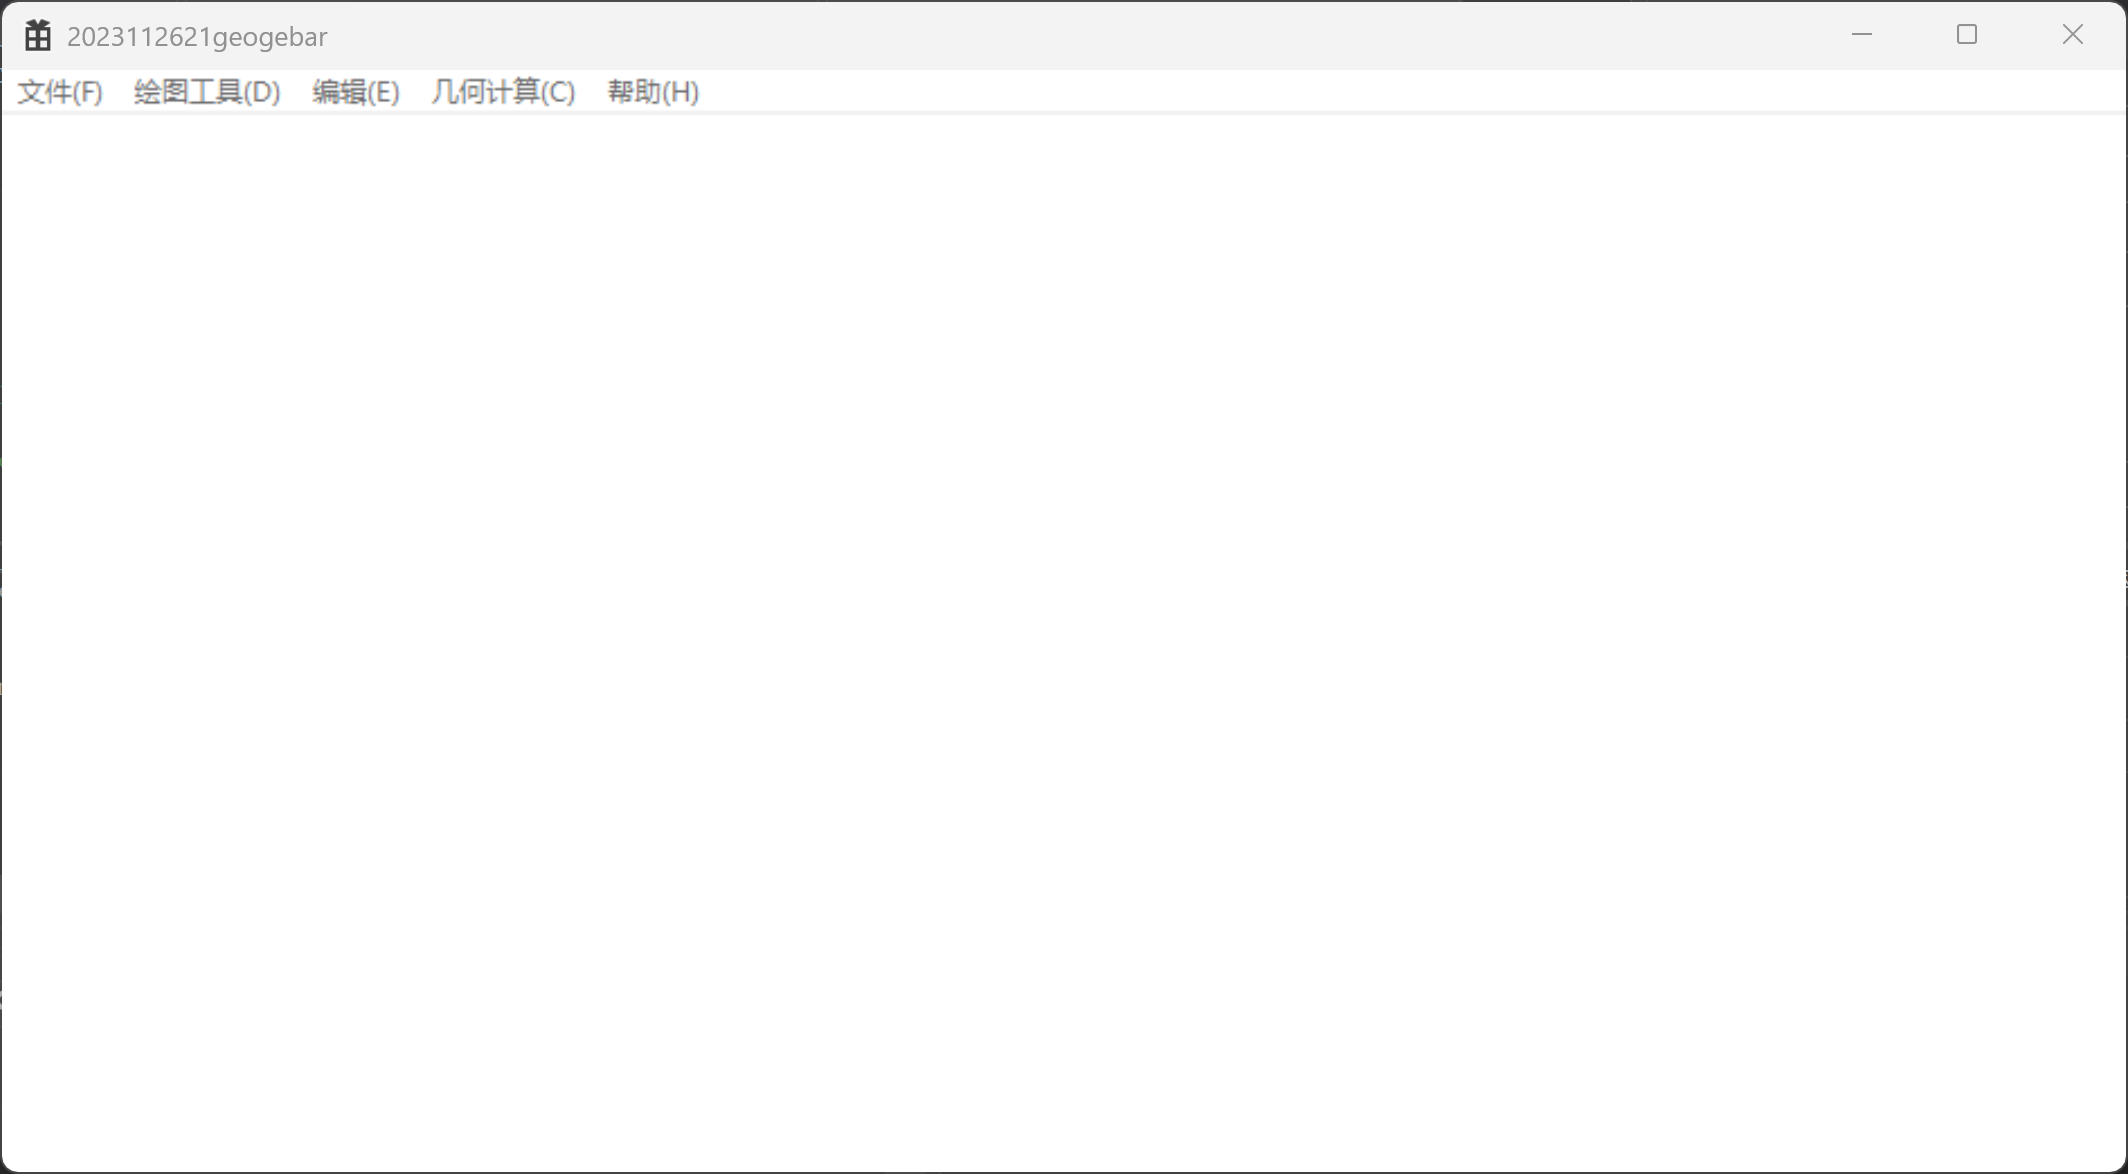
\includegraphics[width=0.92\textwidth]{images/jiemian.png}
\caption{程序界面示例}
\end{figure}

\end{tcolorbox}

\subsection{绘制基本图形}

\begin{tcolorbox}
\textbf{1. 绘制直线}
\begin{enumerate}
    \item 点击菜单"绘制→直线"
    \item 在画布上点击鼠标左键确定起点
    \item 移动鼠标，可看到虚线预览
    \item 再次点击鼠标左键确定终点，完成直线绘制
    \item 按ESC键或右键可取消当前操作
\end{enumerate}

% 在此处插入绘制直线的截图
\begin{figure}[H]
	\centering
	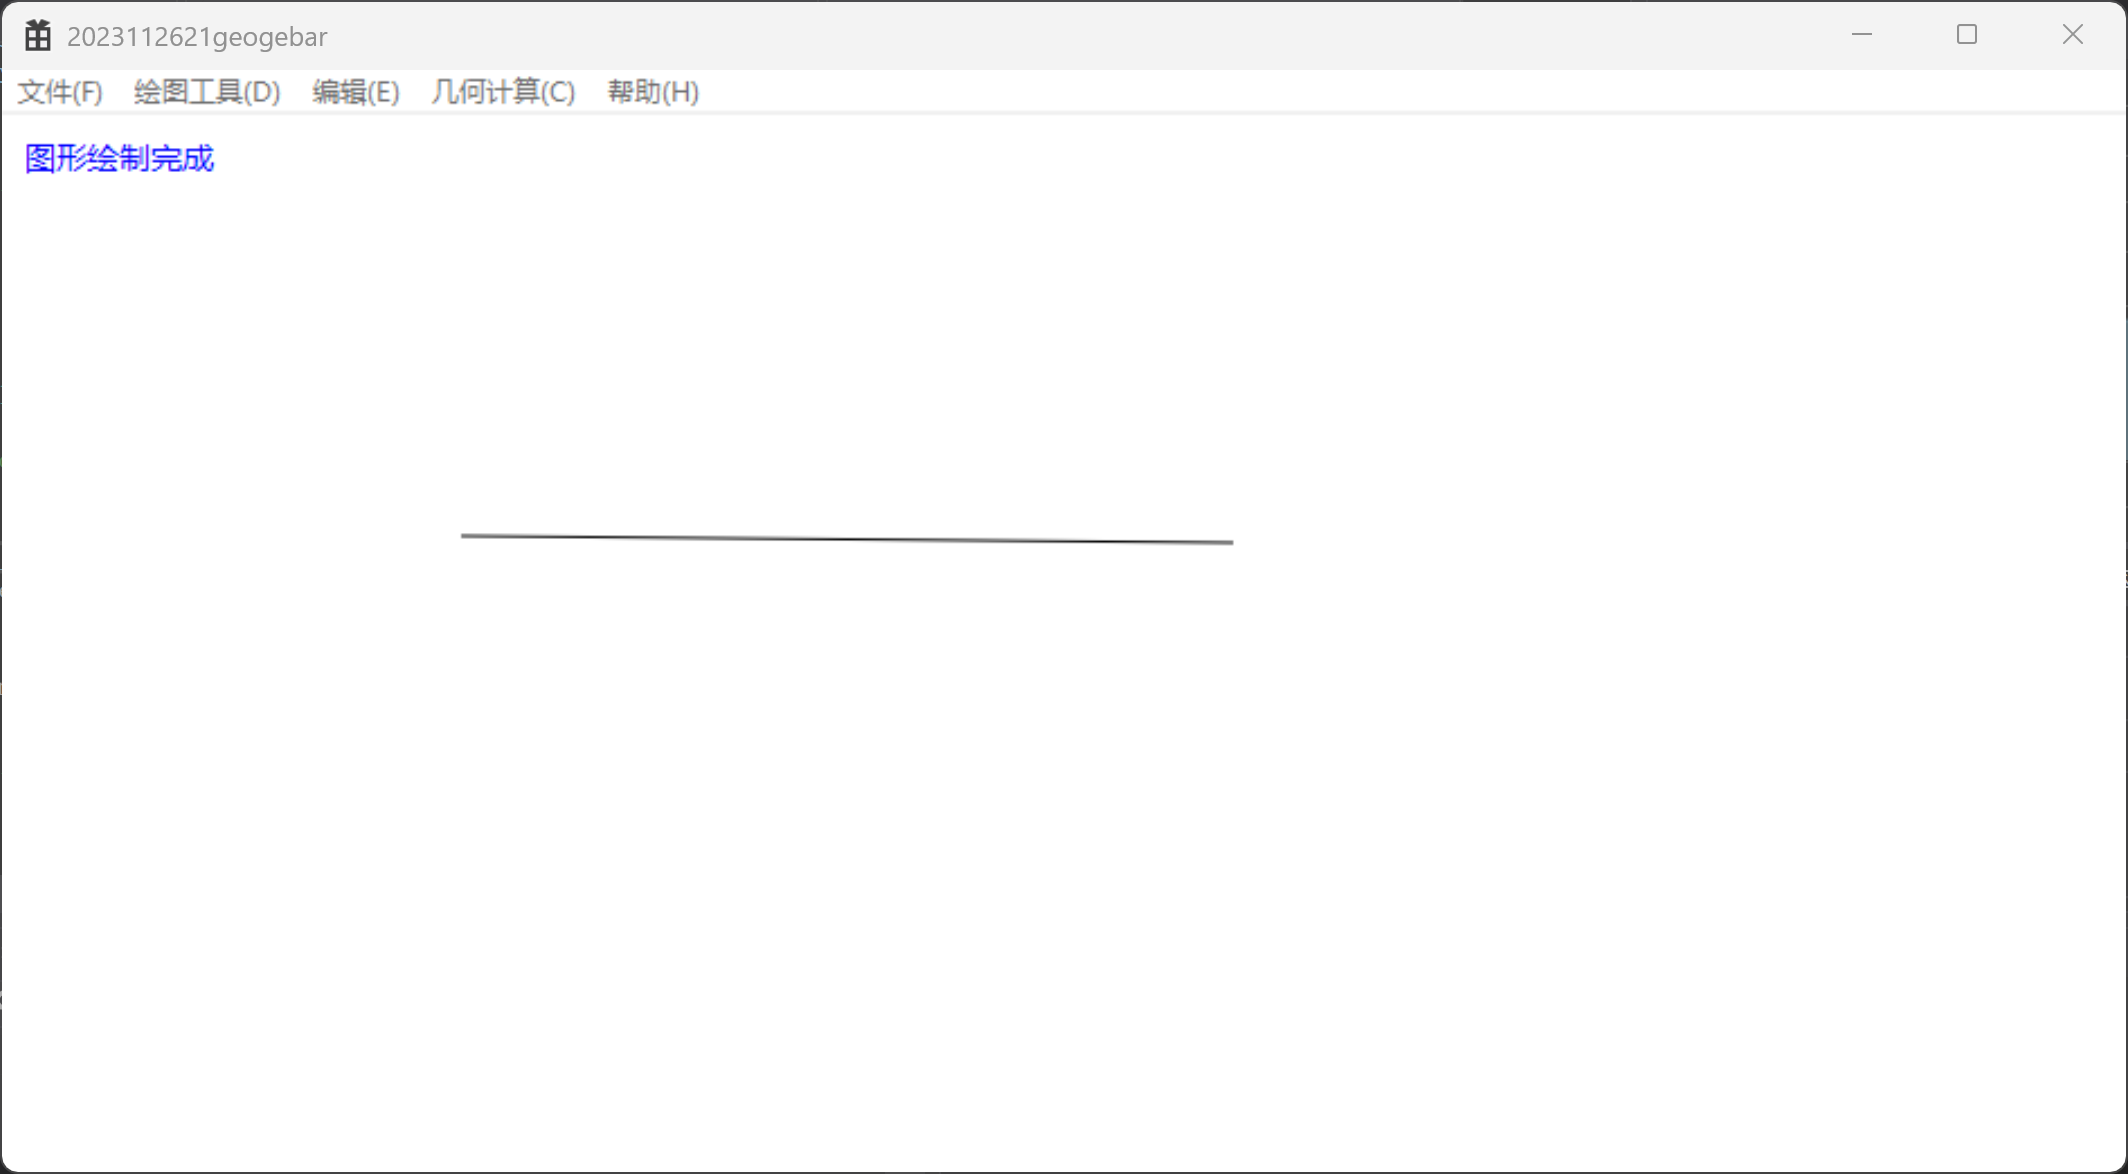
\includegraphics[width=0.92\textwidth]{images/huazhixian.png}
	\caption{绘制直线示例}
\end{figure}

\textbf{2. 绘制圆}
\begin{enumerate}
    \item 点击菜单"绘制→圆"
    \item 在画布上点击鼠标左键确定圆心
    \item 移动鼠标，可看到圆的虚线预览，半径随鼠标位置变化
    \item 再次点击鼠标左键确定半径，完成圆的绘制
\end{enumerate}

% 在此处插入绘制圆的截图
\begin{figure}[H]
	\centering
	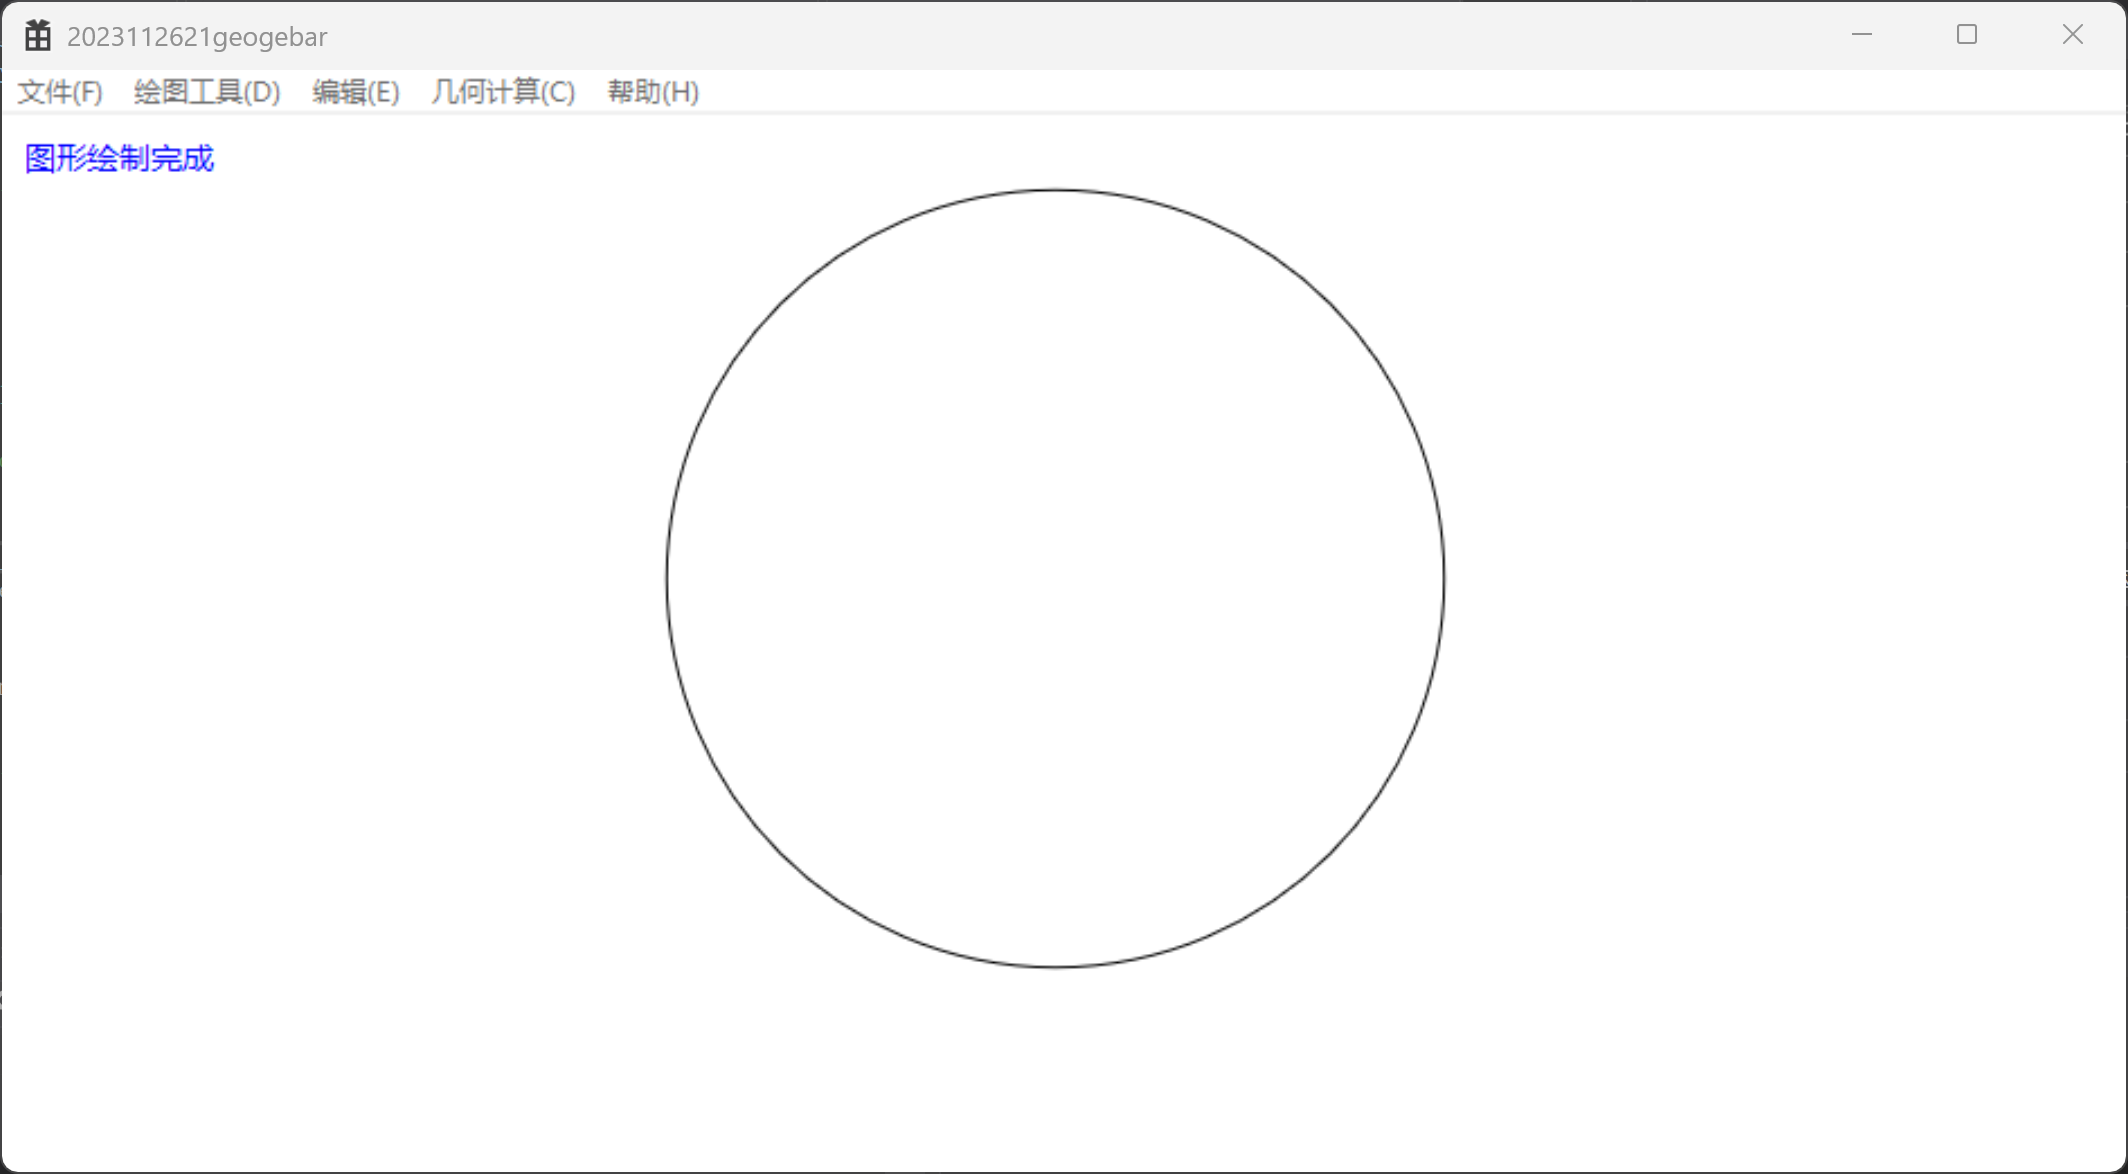
\includegraphics[width=0.92\textwidth]{images/huayuan.png}
	\caption{绘制圆示例}
\end{figure}

\textbf{3. 绘制矩形}
\begin{enumerate}
    \item 点击菜单"绘制→矩形"
    \item 在画布上点击鼠标左键确定第一个角点
    \item 移动鼠标，可看到矩形的虚线预览
    \item 再次点击鼠标左键确定对角点，完成矩形绘制
\end{enumerate}

% 在此处插入绘制矩形的截图
\begin{figure}[H]
	\centering
	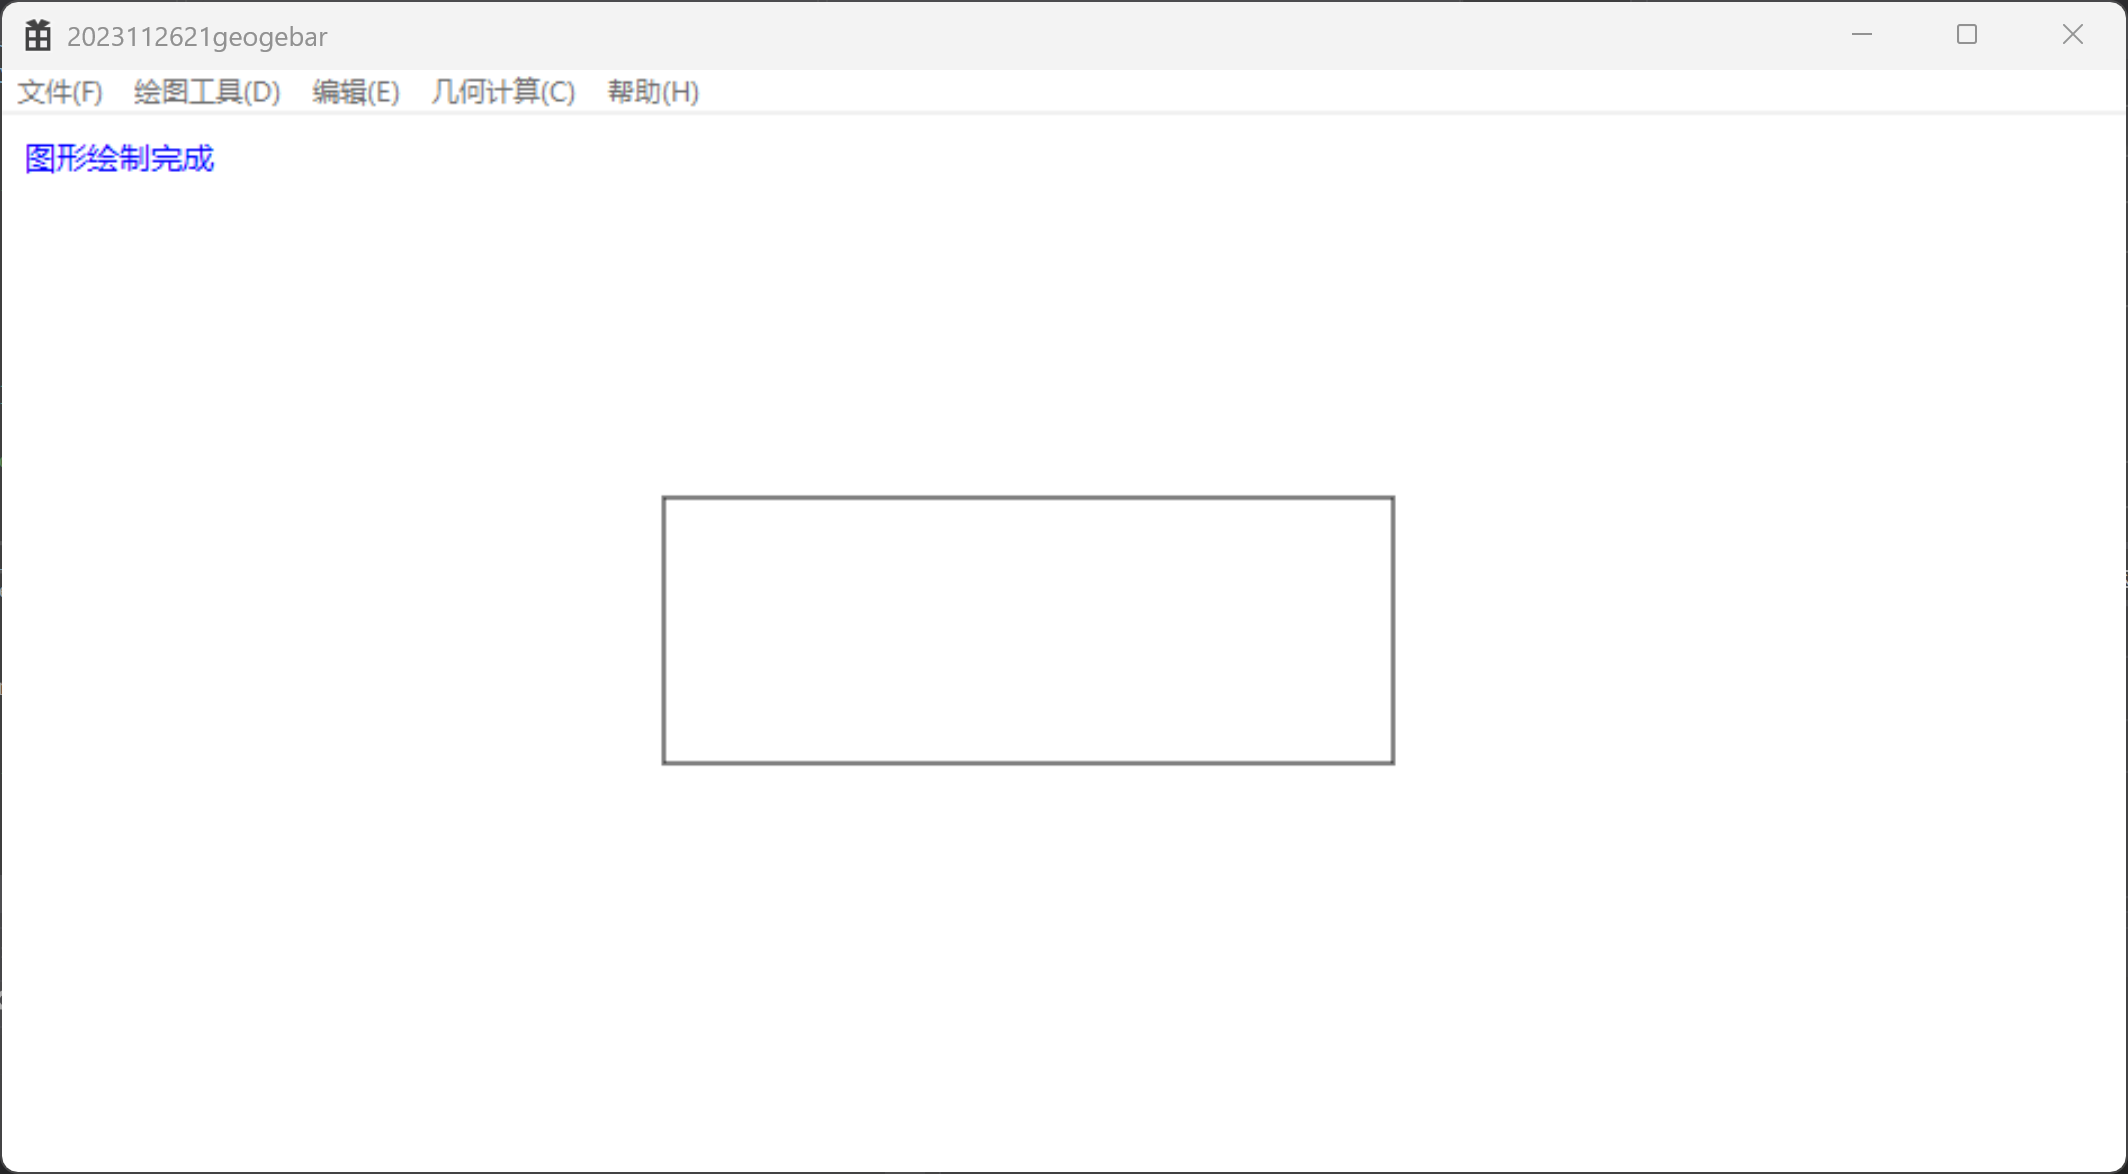
\includegraphics[width=0.92\textwidth]{images/huajuxing.png}
	\caption{绘制矩形示例}
\end{figure}

\textbf{4. 绘制三角形}
\begin{enumerate}
    \item 点击菜单"绘制→三角形"
    \item 依次点击三个顶点位置
    \item 第一、二个点之间会显示虚线预览
    \item 点击第三个点后自动完成三角形绘制
\end{enumerate}

% 在此处插入绘制三角形的截图
\begin{figure}[H]
	\centering
	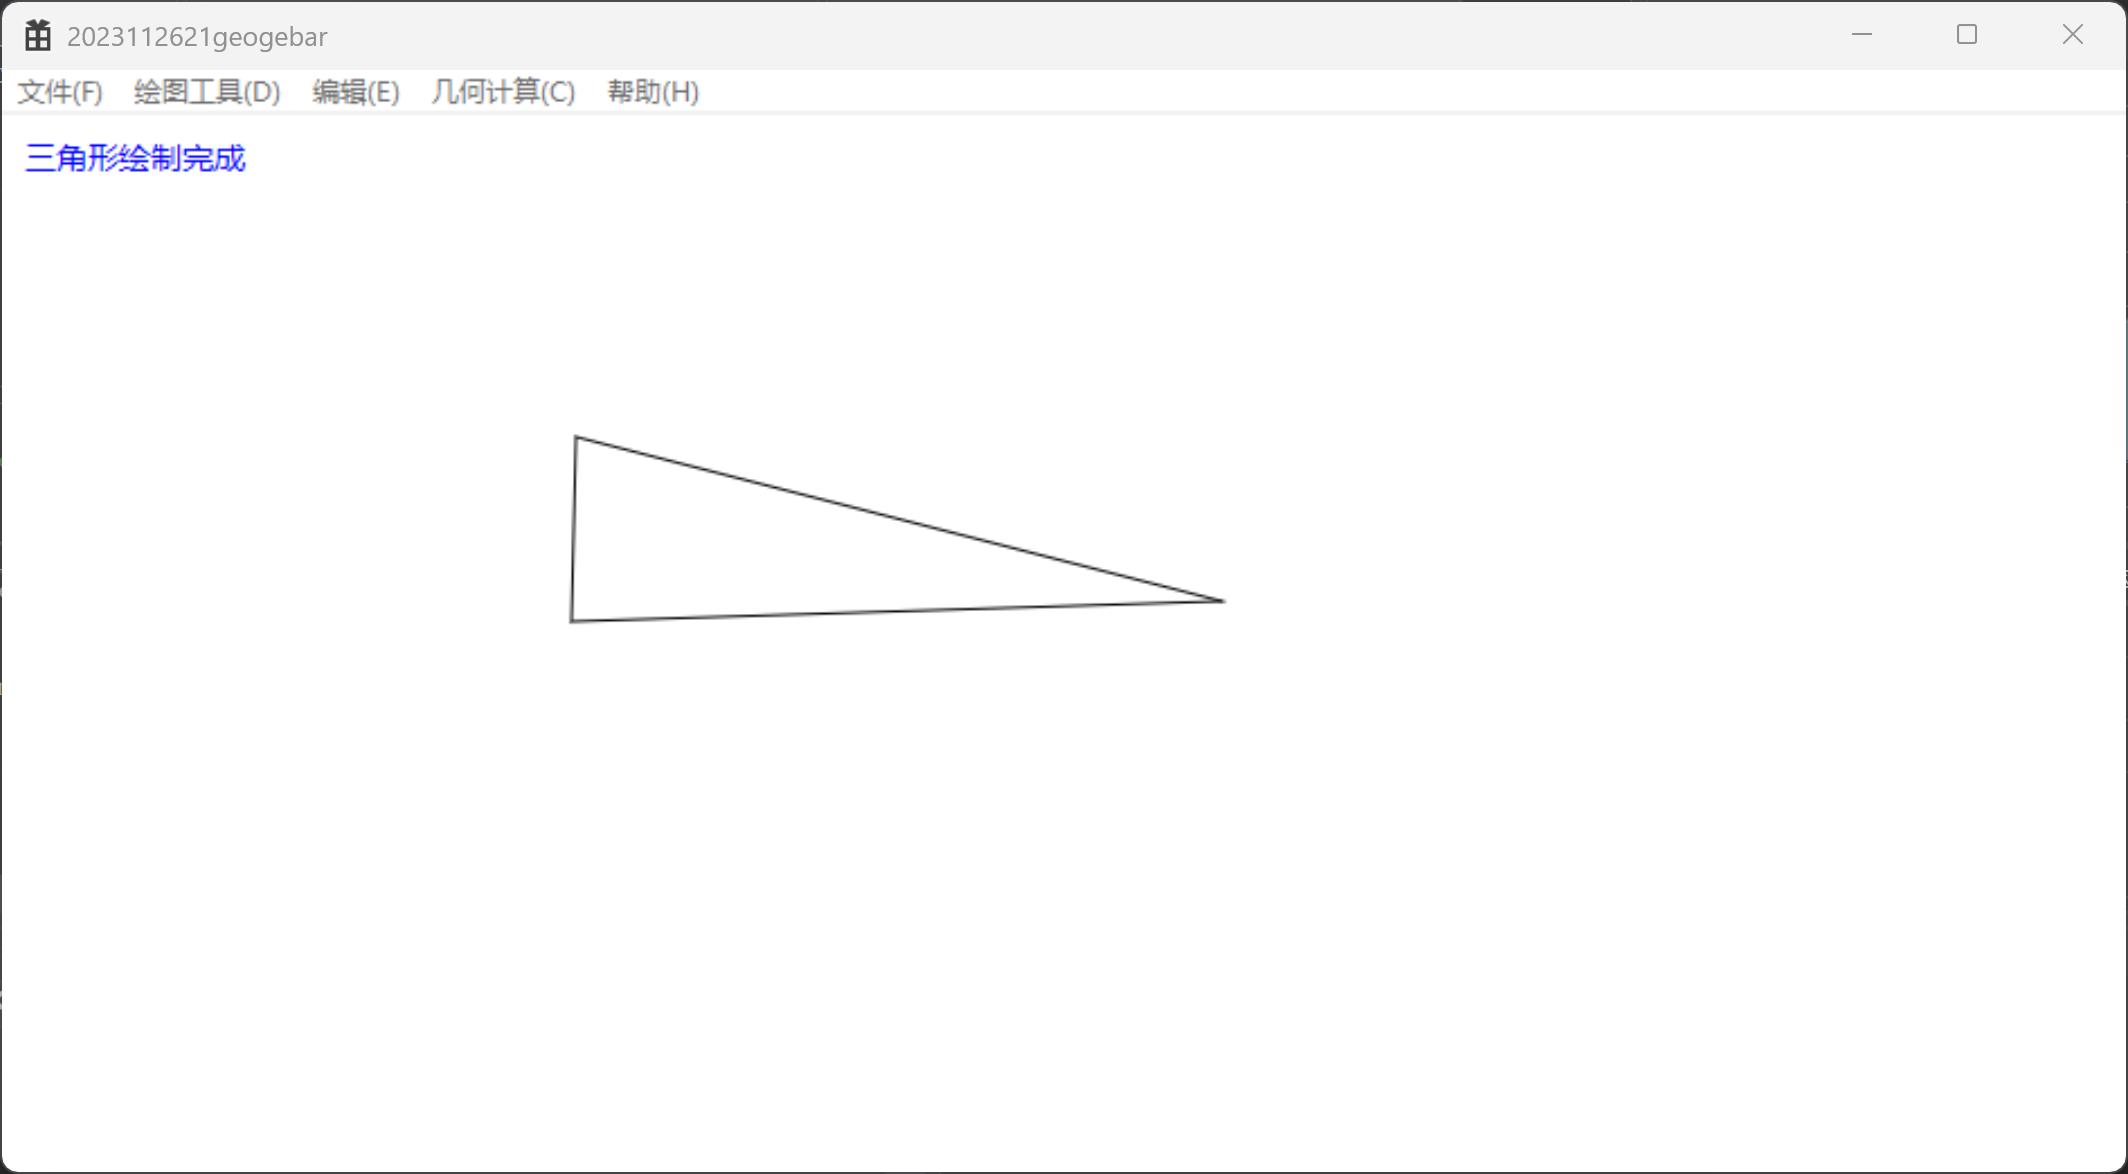
\includegraphics[width=0.92\textwidth]{images/huasanjiaoxing.png}
	\caption{绘制三角形示例}
\end{figure}

\textbf{5. 绘制菱形}
\begin{enumerate}
    \item 点击菜单"绘制→菱形"
    \item 在画布上点击鼠标左键确定中心点
    \item 移动鼠标，菱形大小随鼠标位置变化
    \item 再次点击鼠标左键确定尺寸，完成菱形绘制
\end{enumerate}

% 在此处插入绘制菱形的截图
\begin{figure}[H]
	\centering
	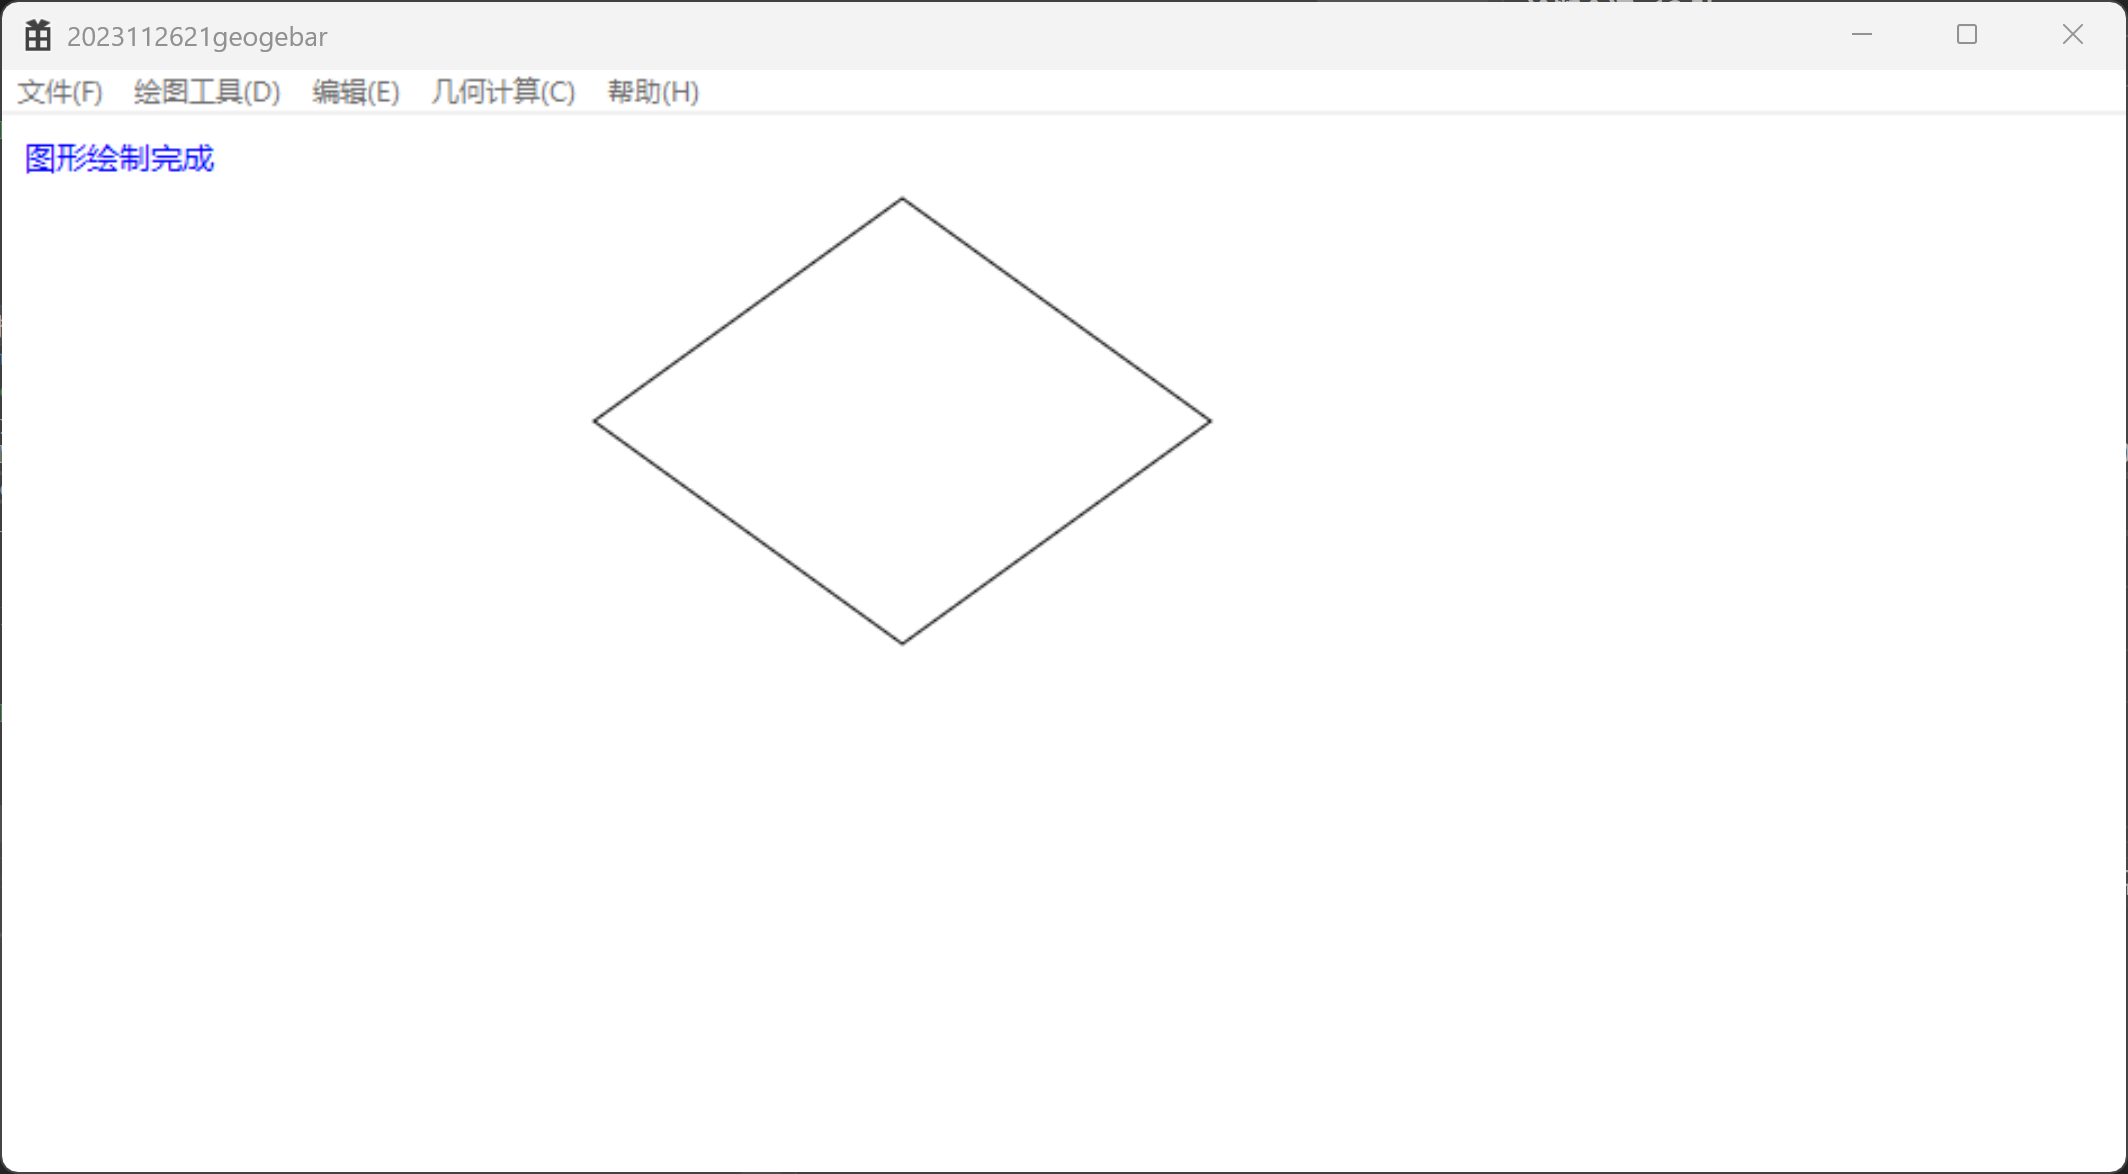
\includegraphics[width=0.92\textwidth]{images/hualingxing.png}
	\caption{绘制菱形示例}
\end{figure}

\textbf{6. 绘制平行四边形}
\begin{enumerate}
    \item 点击菜单"绘制→平行四边形"
    \item 依次点击三个顶点
    \item 系统自动计算并绘制第四个顶点
    \item 完成平行四边形绘制
\end{enumerate}

% 在此处插入绘制平行四边形的截图
\begin{figure}[H]
	\centering
	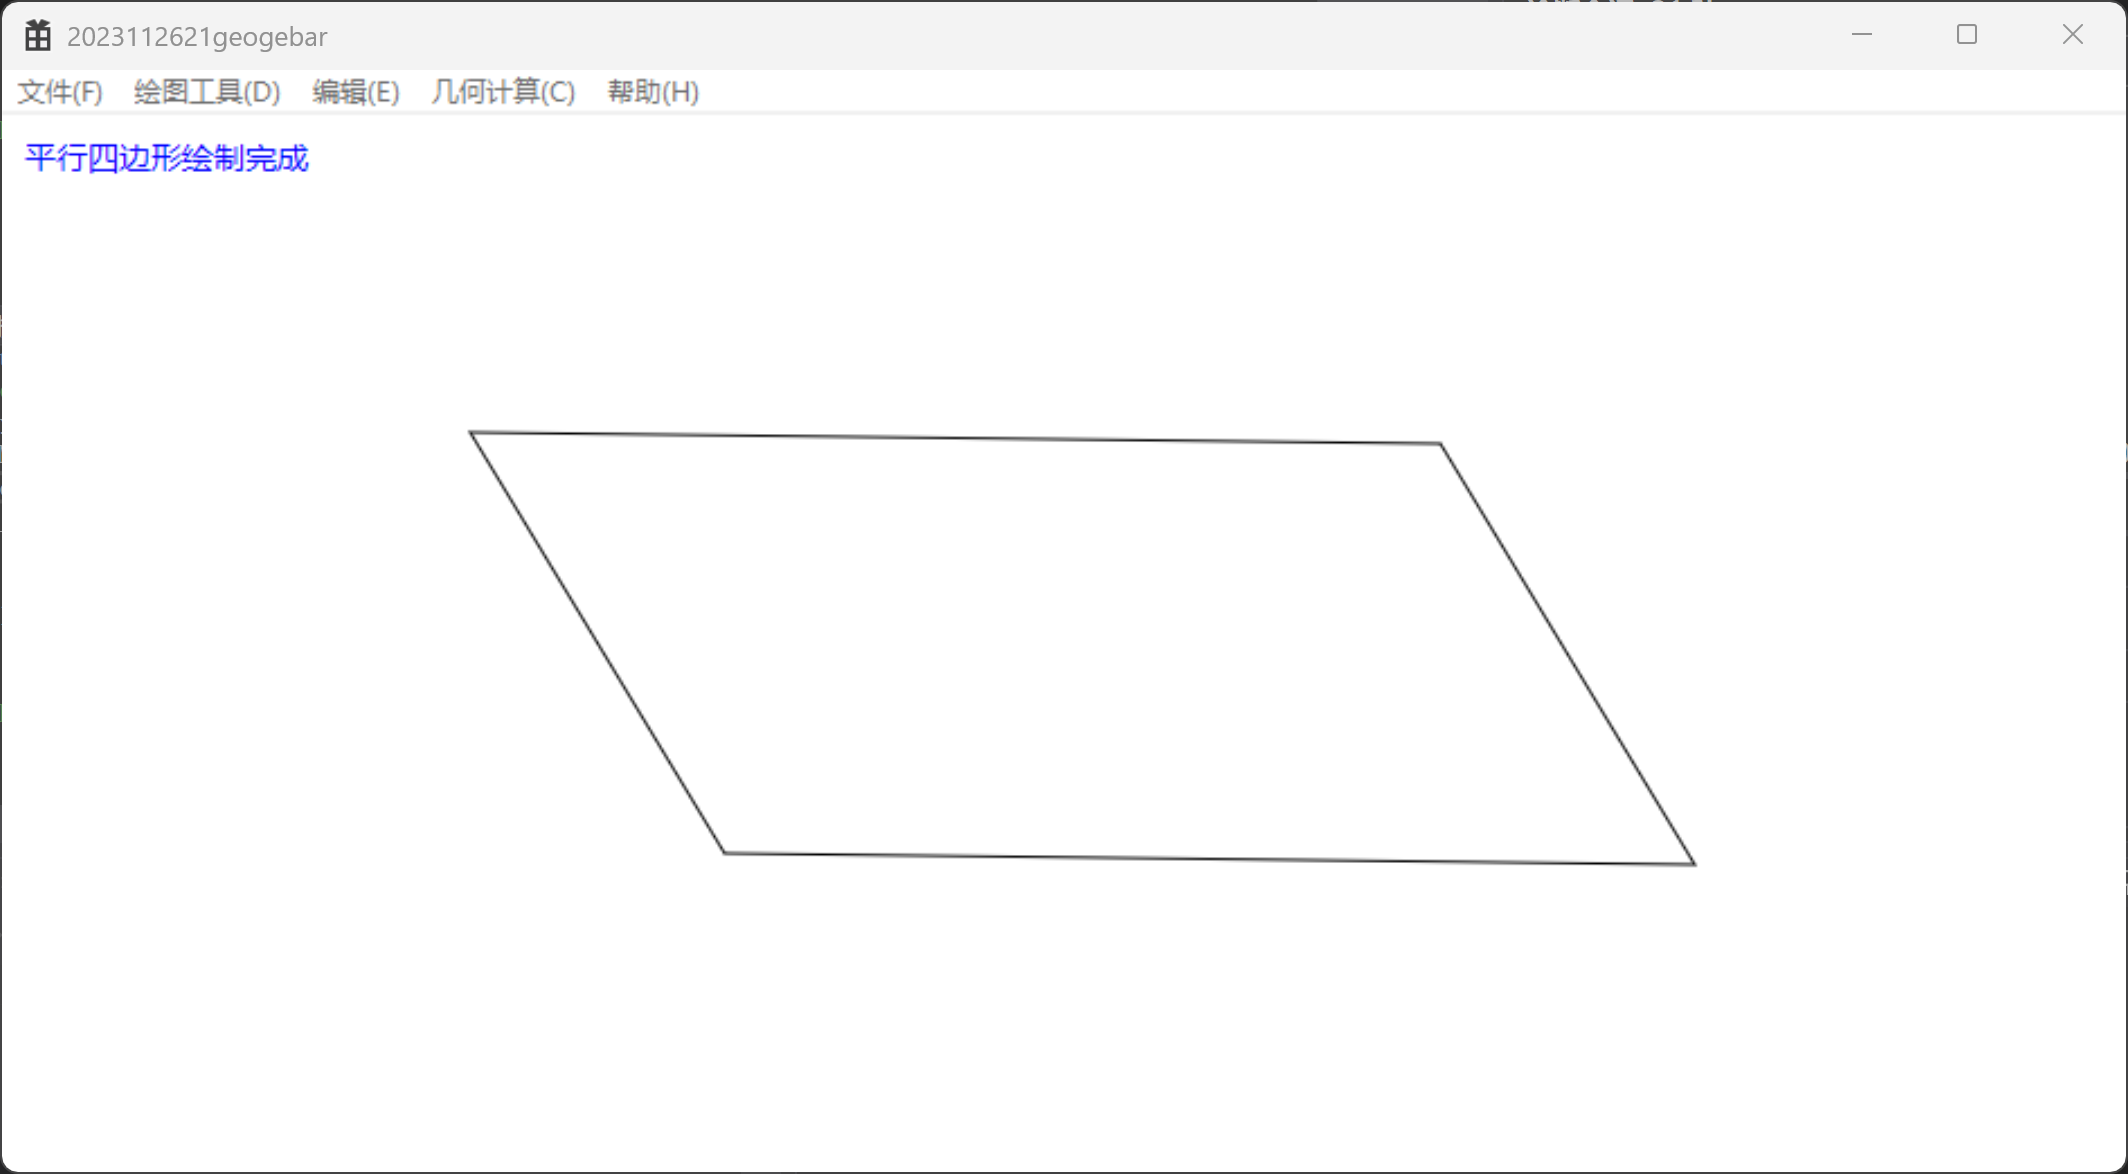
\includegraphics[width=0.92\textwidth]{images/huapingxingsibianxing.png}
	\caption{绘制平行四边形示例}
\end{figure}

\textbf{7. 绘制曲线}
\begin{enumerate}
    \item 点击菜单"绘制→曲线"
    \item 连续点击鼠标左键添加控制点
    \item 每添加一个点，曲线会实时更新
    \item 右键点击或双击完成曲线绘制
    \item 至少需要2个点才能形成有效曲线
\end{enumerate}

\begin{figure}[H]
	\centering
	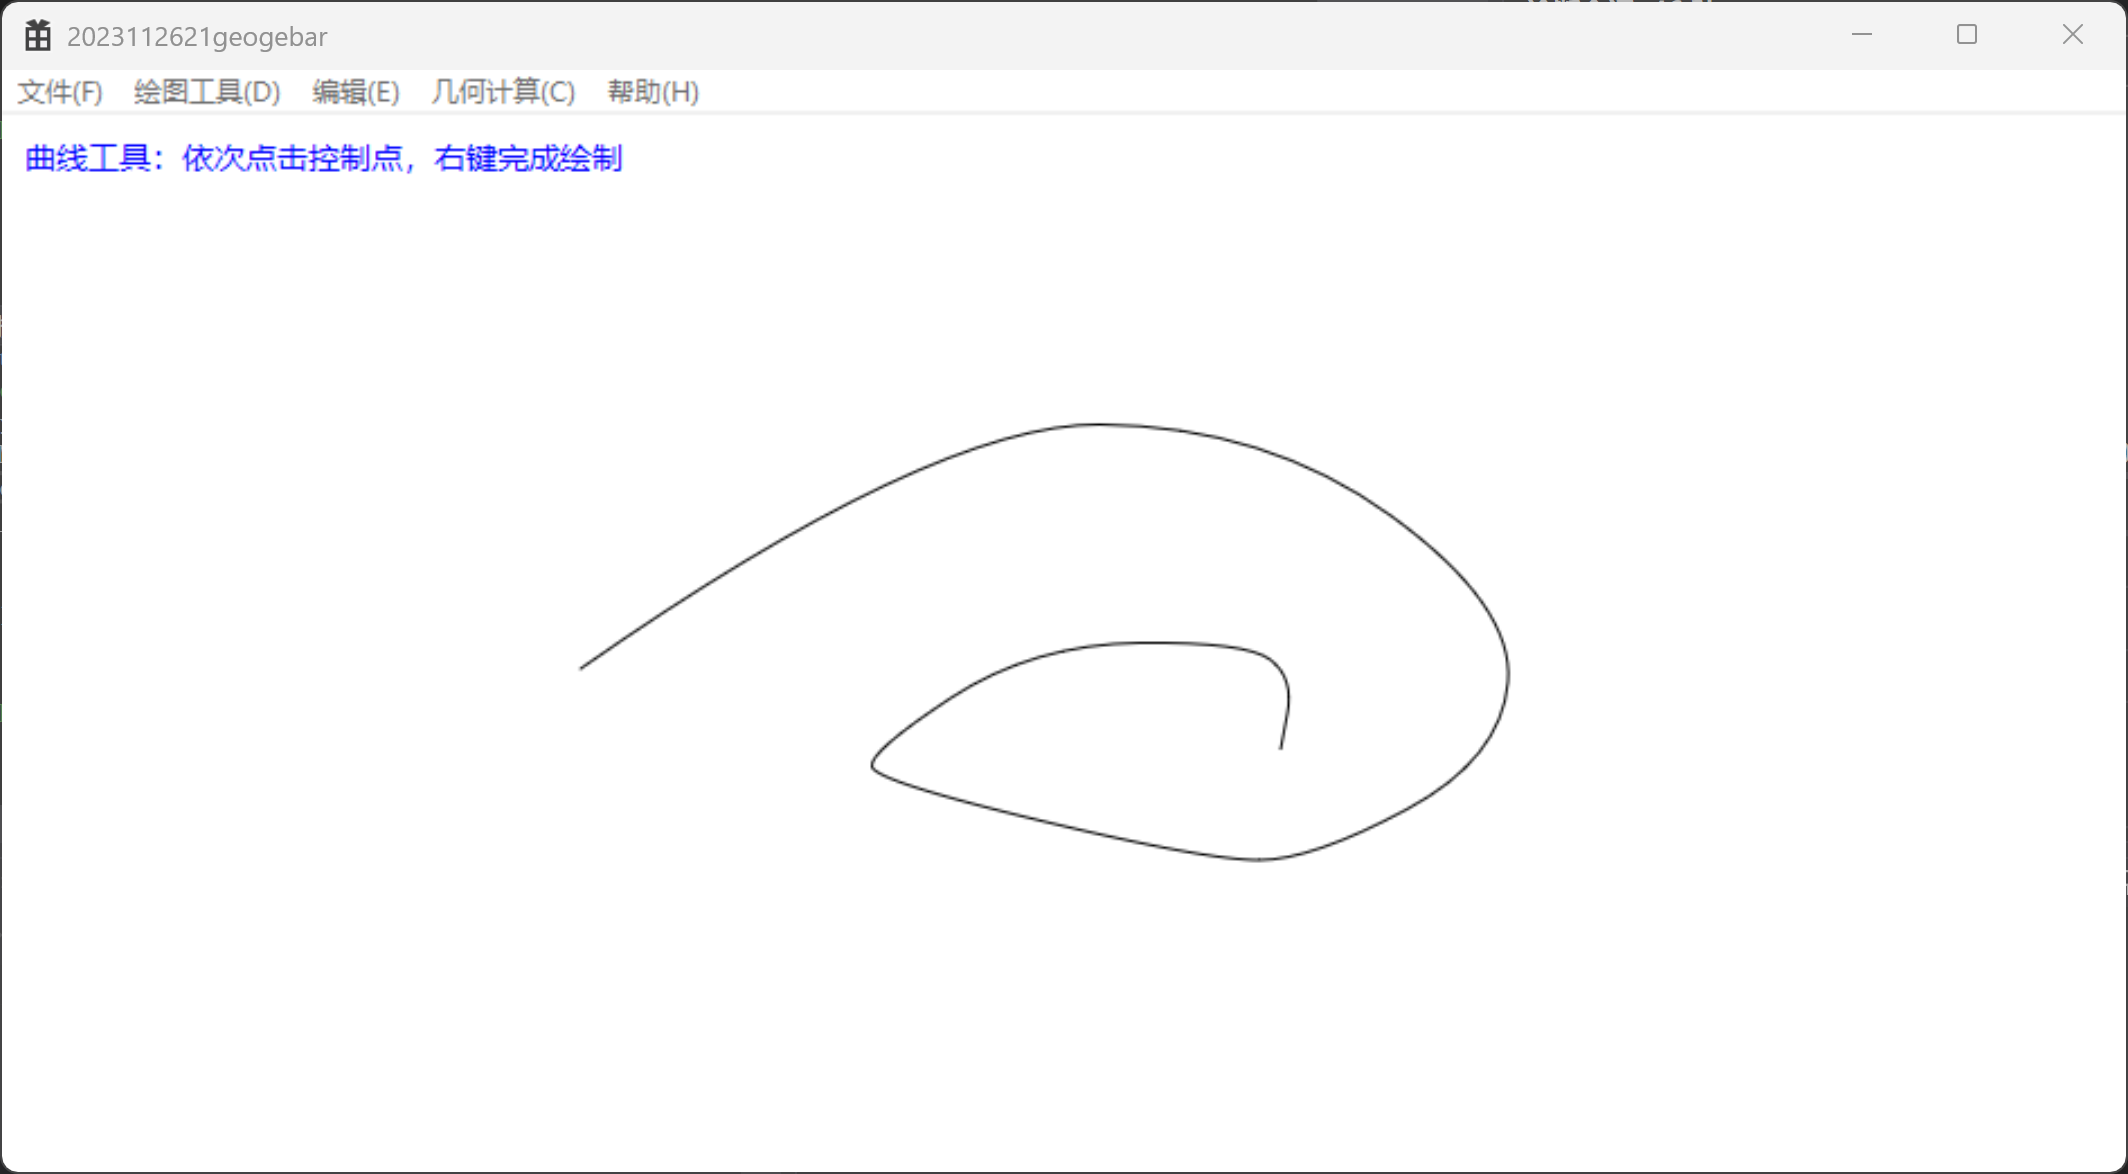
\includegraphics[width=0.92\textwidth]{images/huaquxian.png}
	\caption{绘制曲线示例}
\end{figure}

\textbf{8. 绘制多义线}
\begin{enumerate}
    \item 点击菜单"绘制→多义线"
    \item 连续点击鼠标左键添加顶点
    \item 每添加一个点，会用直线连接到前一个点
    \item 右键点击或双击完成多义线绘制
\end{enumerate}

\begin{figure}[H]
	\centering
	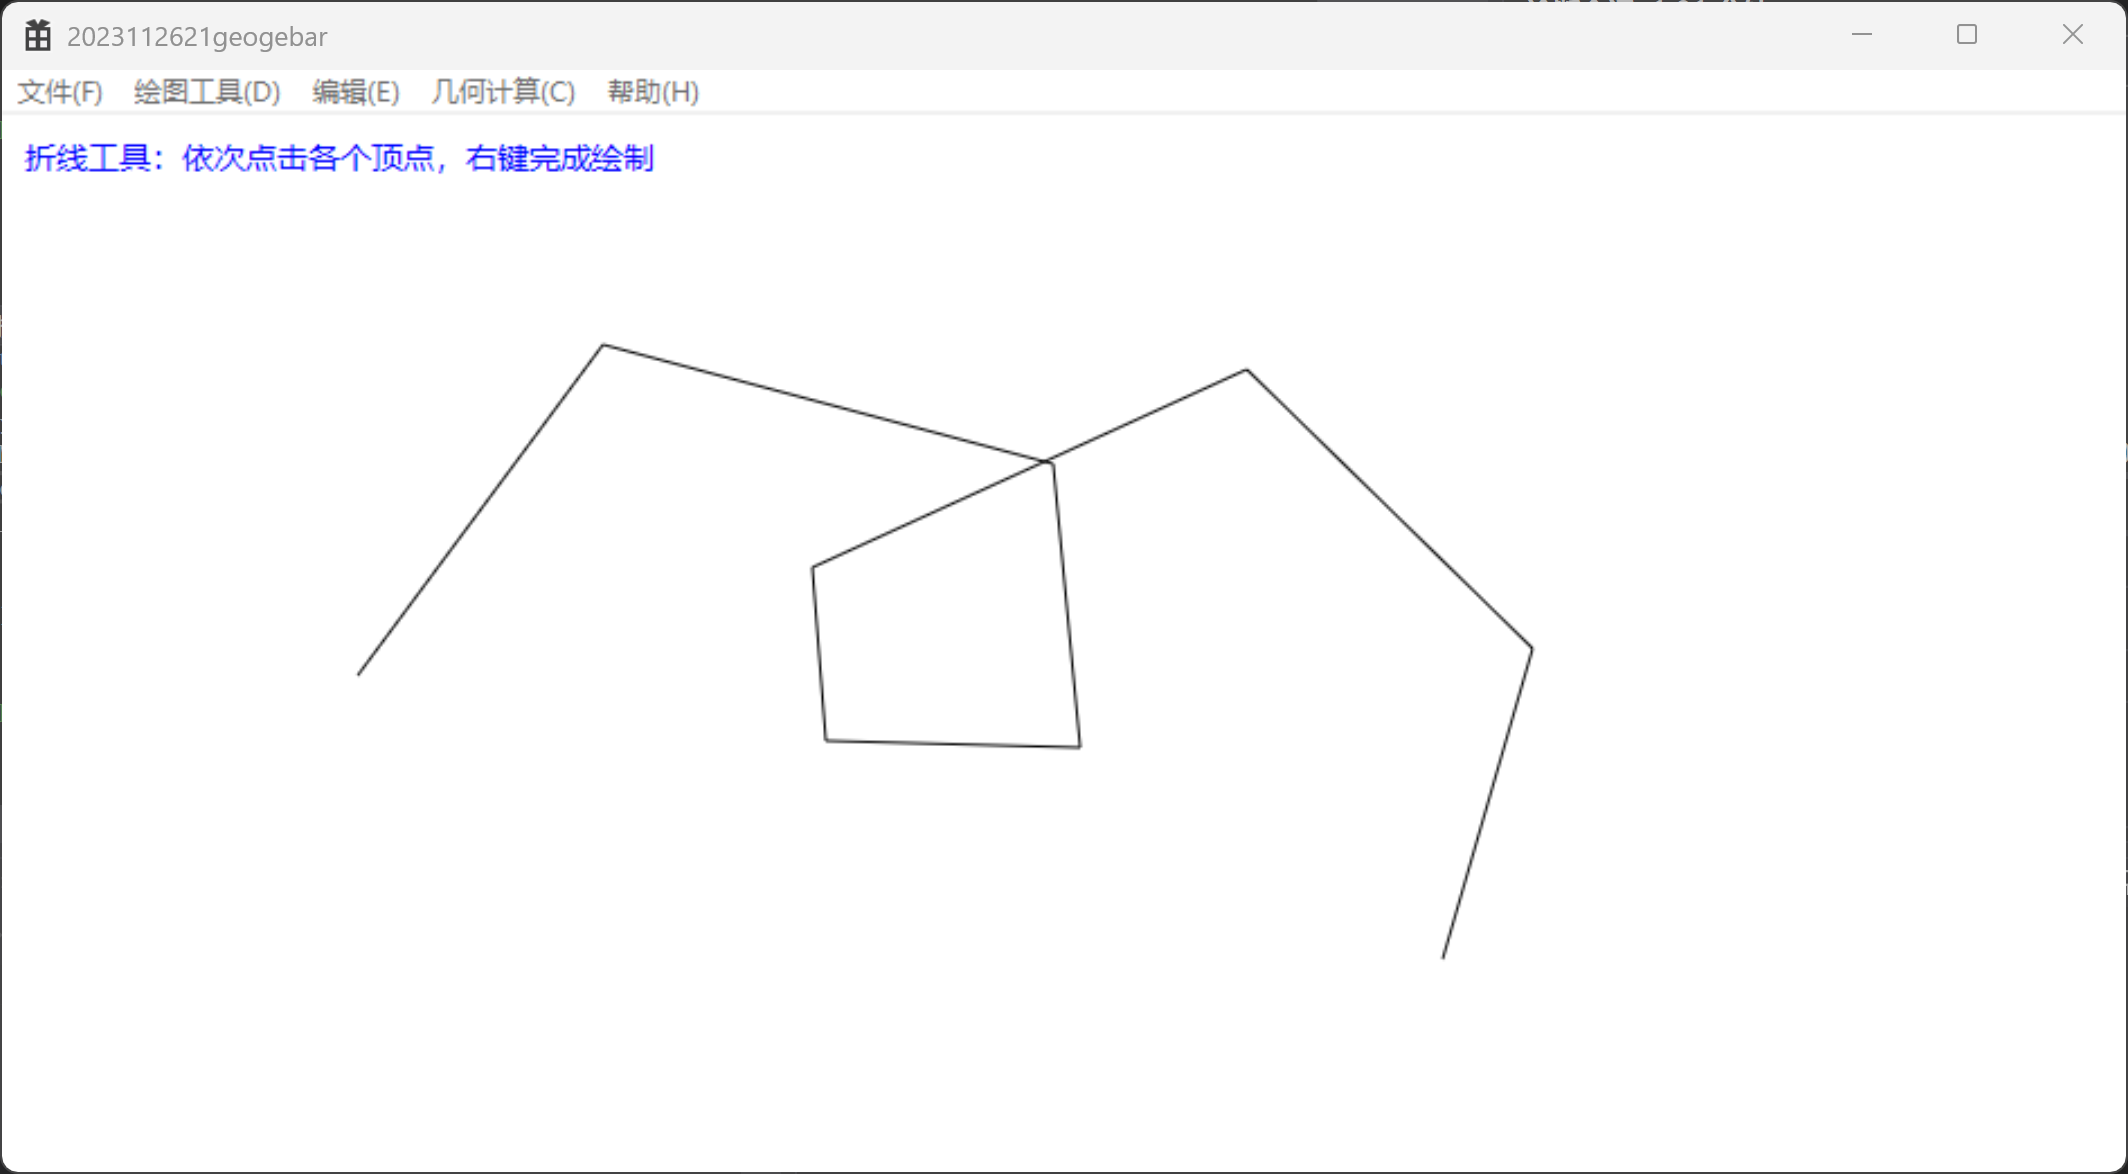
\includegraphics[width=0.92\textwidth]{images/huaduoyixian.png}
	\caption{绘制多义线示例}
\end{figure}
\end{tcolorbox}

\subsection{选择与编辑图形}

\begin{tcolorbox}
\textbf{1. 选择图形}
\begin{enumerate}
    \item 点击菜单"编辑→选择"进入选择模式
    \item 将鼠标移动到图形上，光标变为手型
    \item 点击图形，选中的图形会以红色虚线显示
    \item 点击空白区域或按ESC键取消选择
\end{enumerate}

\begin{figure}[H]
	\centering
	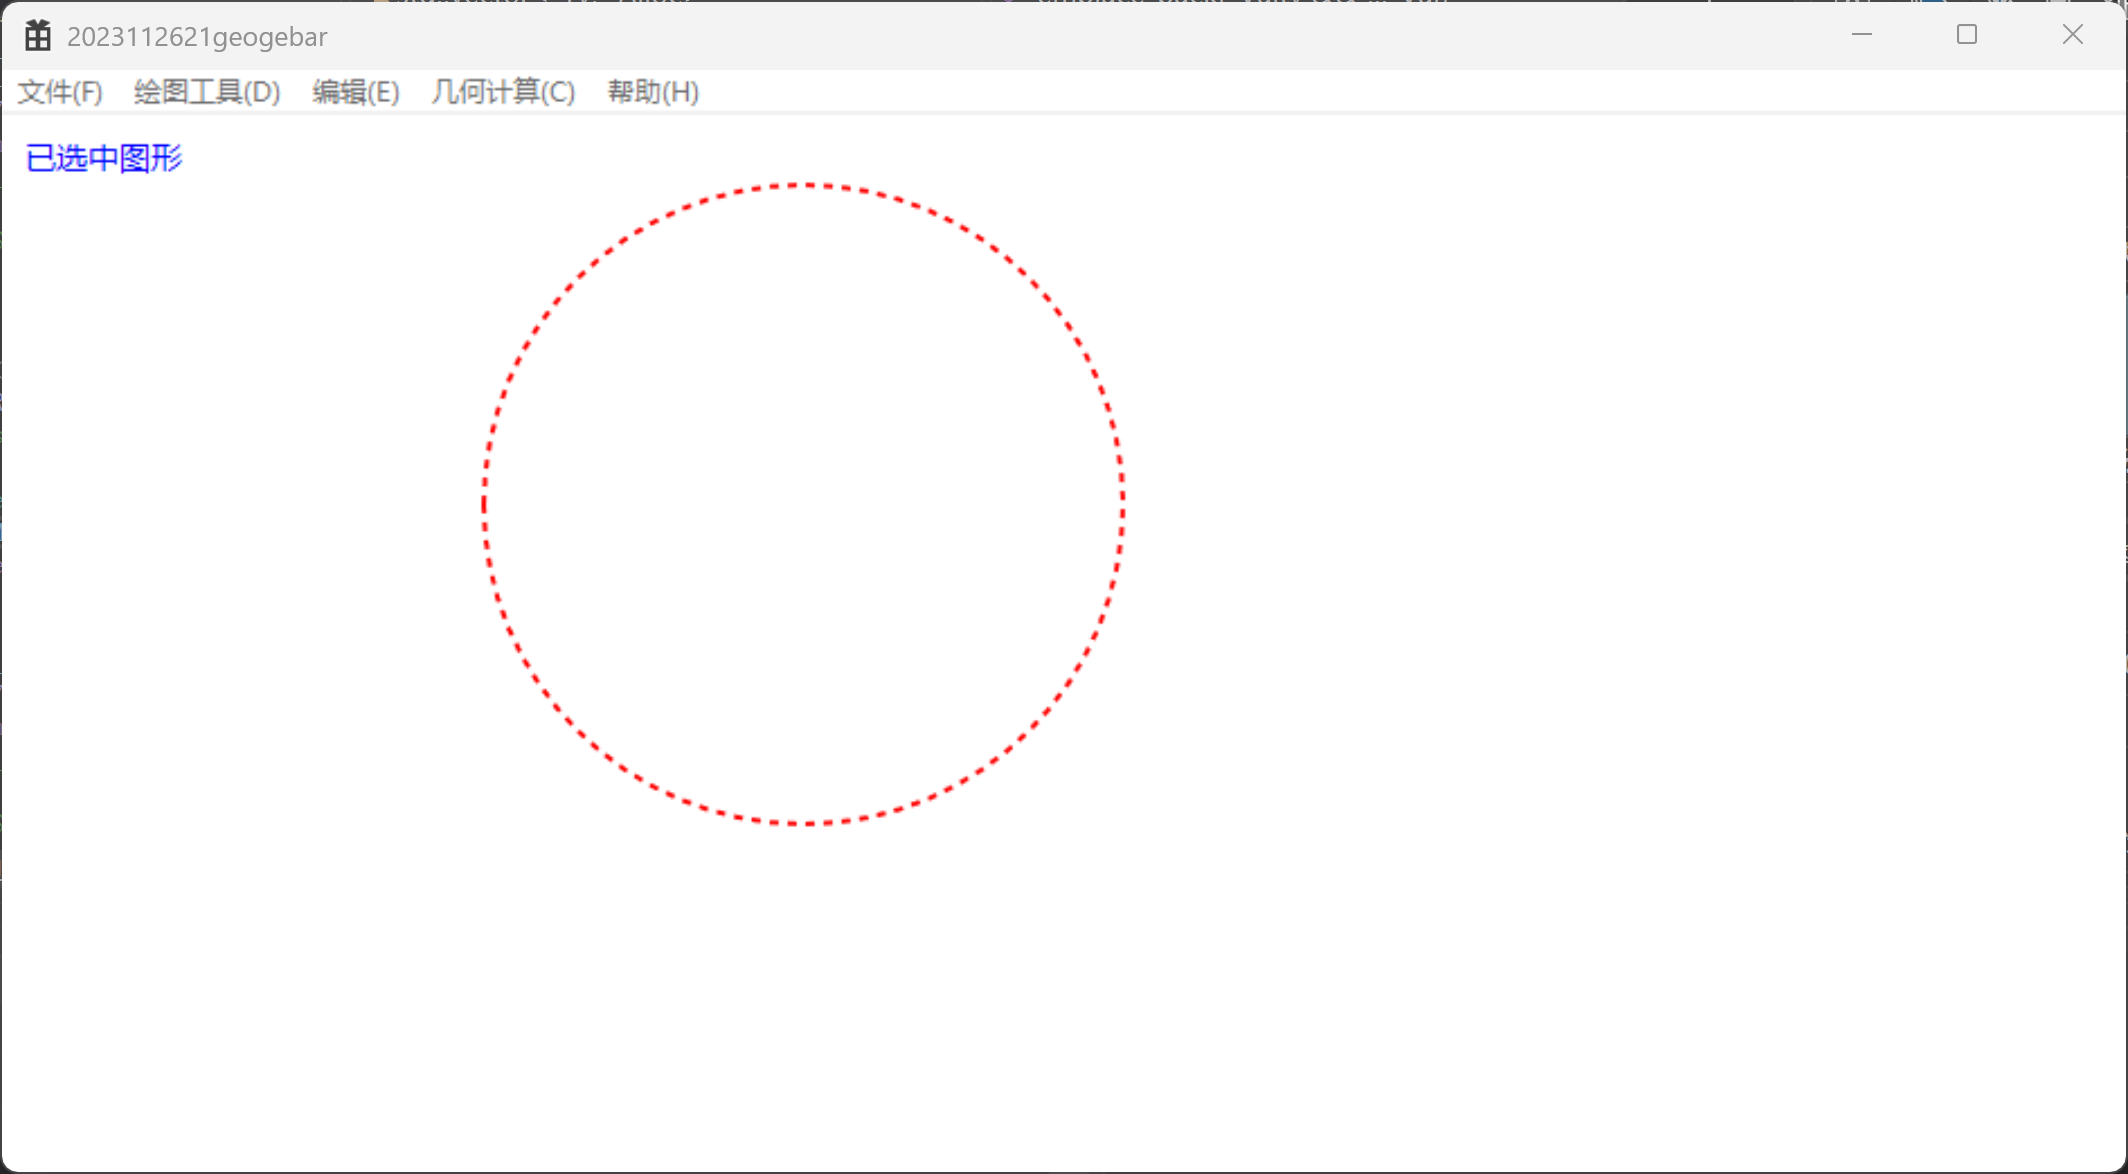
\includegraphics[width=0.92\textwidth]{images/xuanze.png}
	\caption{选择图形示例}
\end{figure}
\begin{figure}[H]
	\centering
	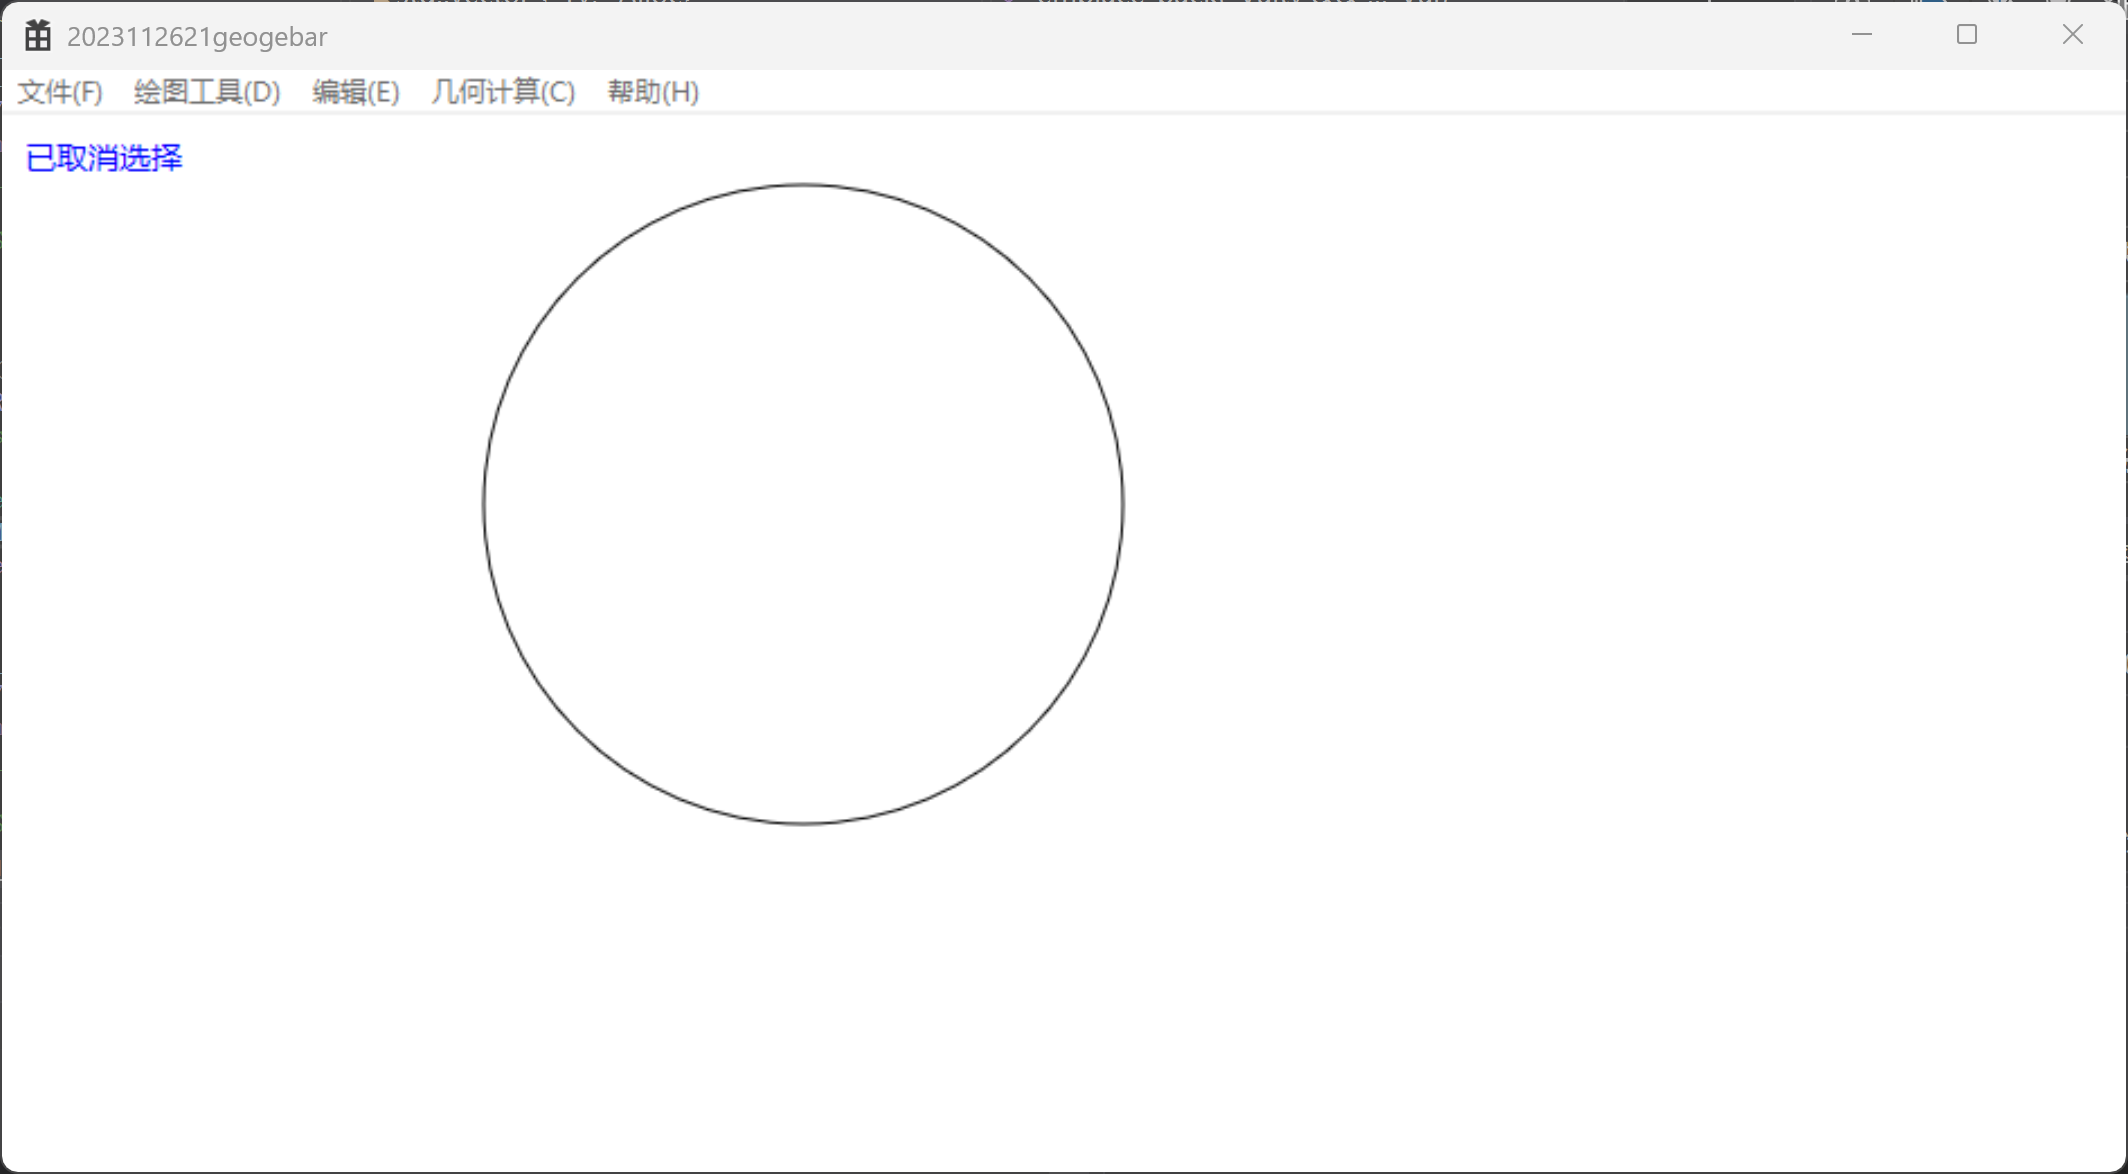
\includegraphics[width=0.92\textwidth]{images/quxiaoxuanze.png}
	\caption{取消选择示例}
\end{figure}

\textbf{2. 移动图形}
\begin{enumerate}
    \item 先选中要移动的图形
    \item 点击菜单"编辑→移动"
    \item 按住鼠标左键拖动图形到目标位置
    \item 释放鼠标左键完成移动
    \item 移动过程中图形会实时跟随鼠标移动
\end{enumerate}

\begin{figure}[H]
	\centering
	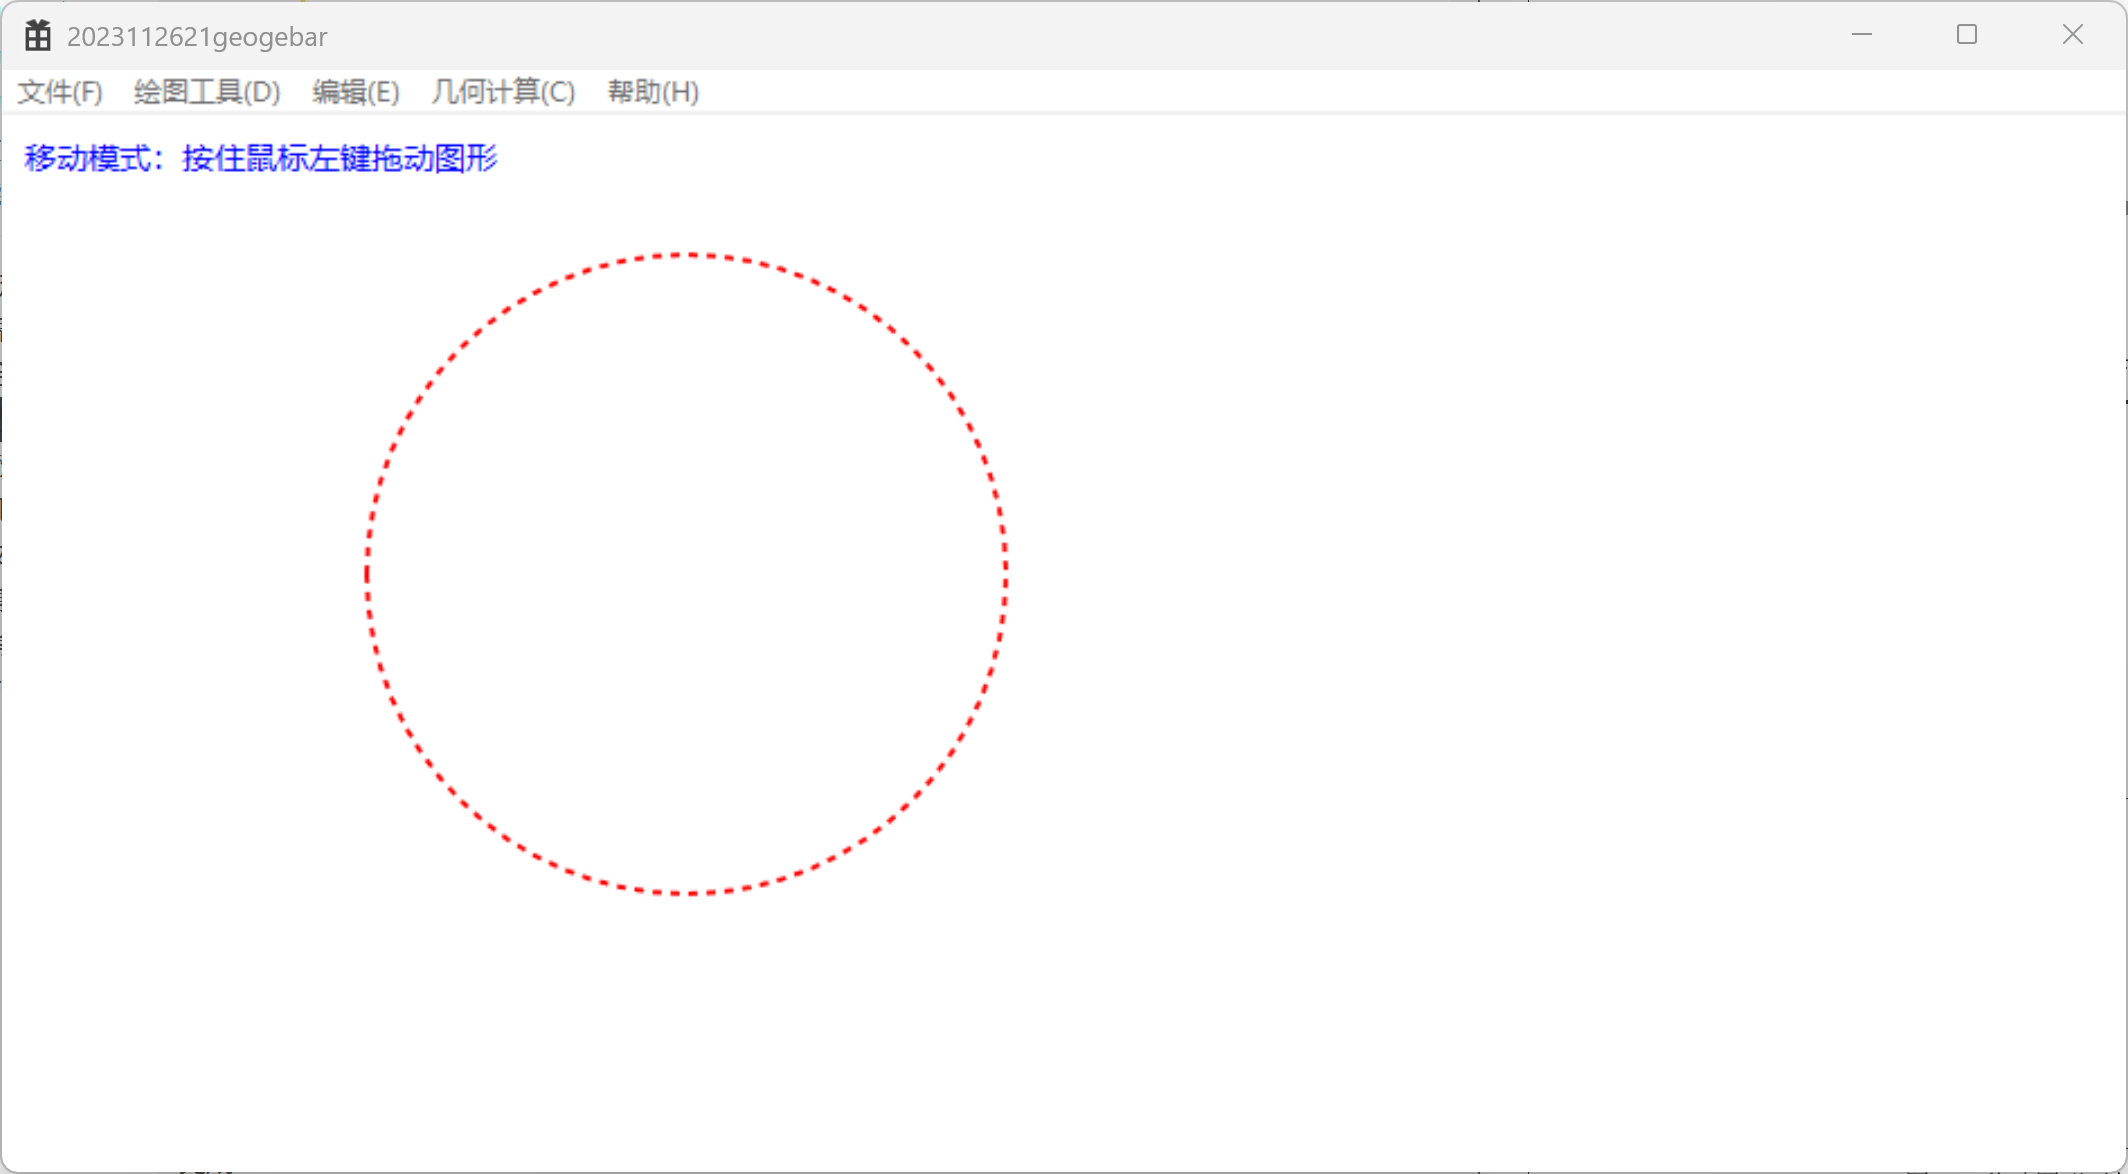
\includegraphics[width=0.92\textwidth]{images/yidong.png}
	\caption{移动图形示例}
\end{figure}

\textbf{3. 旋转图形}
\begin{enumerate}
    \item 先选中要旋转的图形
    \item 点击菜单"编辑→旋转"
    \item 滚动鼠标滚轮调整旋转角度
    \begin{itemize}
        \item 向上滚动：逆时针旋转
        \item 向下滚动：顺时针旋转
    \end{itemize}
    \item 旋转过程中可实时预览效果
    \item 点击鼠标左键确认旋转
    \item 点击鼠标右键取消旋转，恢复原状
\end{enumerate}

\begin{figure}[H]
	\centering
	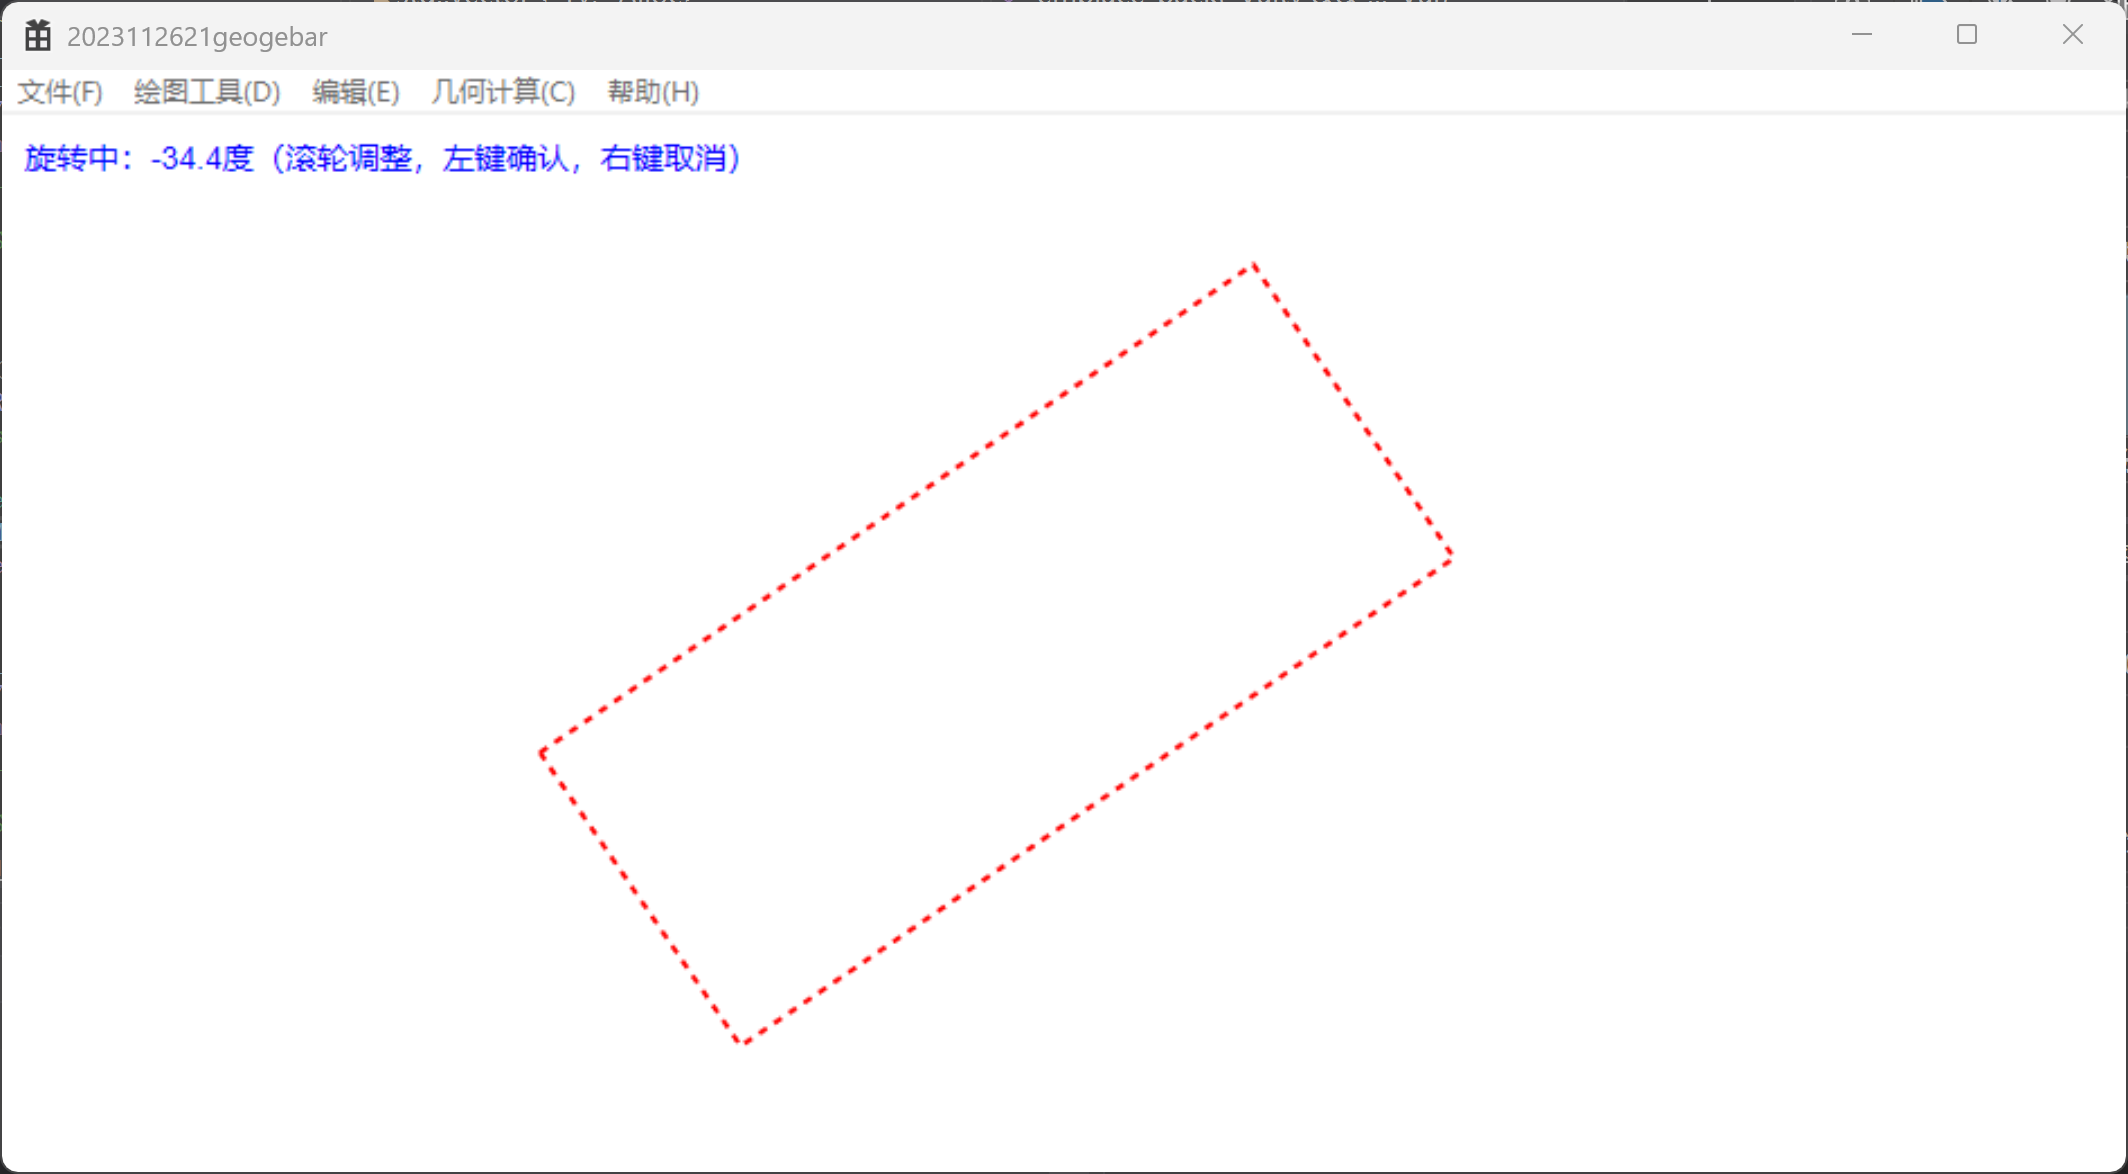
\includegraphics[width=0.92\textwidth]{images/xz1.png}
	\caption{旋转图形示例}
\end{figure}
\begin{figure}[H]
	\centering
	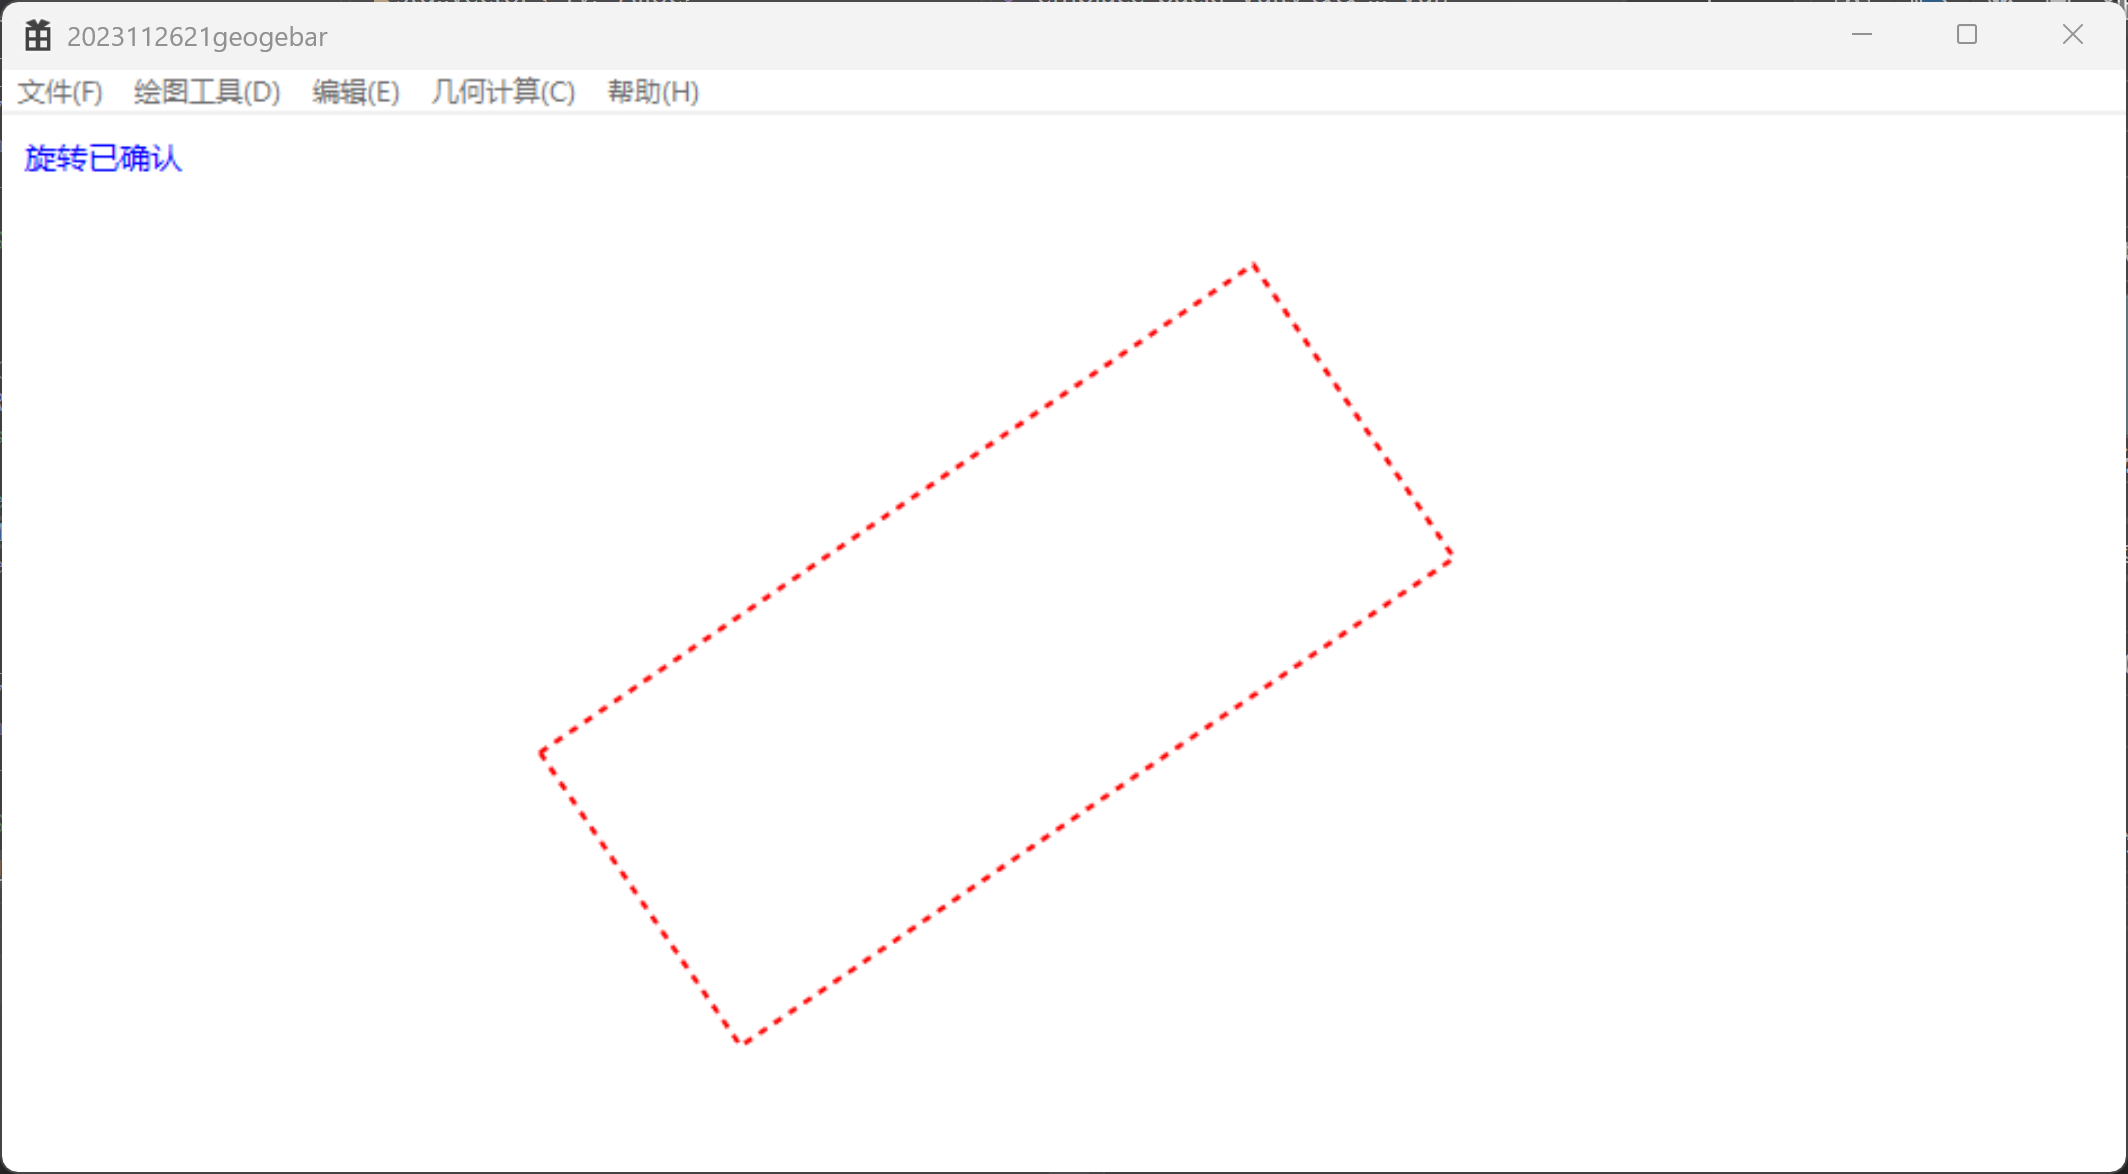
\includegraphics[width=0.92\textwidth]{images/xz2.png}
	\caption{旋转图形示例}
\end{figure}
\begin{figure}[H]
	\centering
	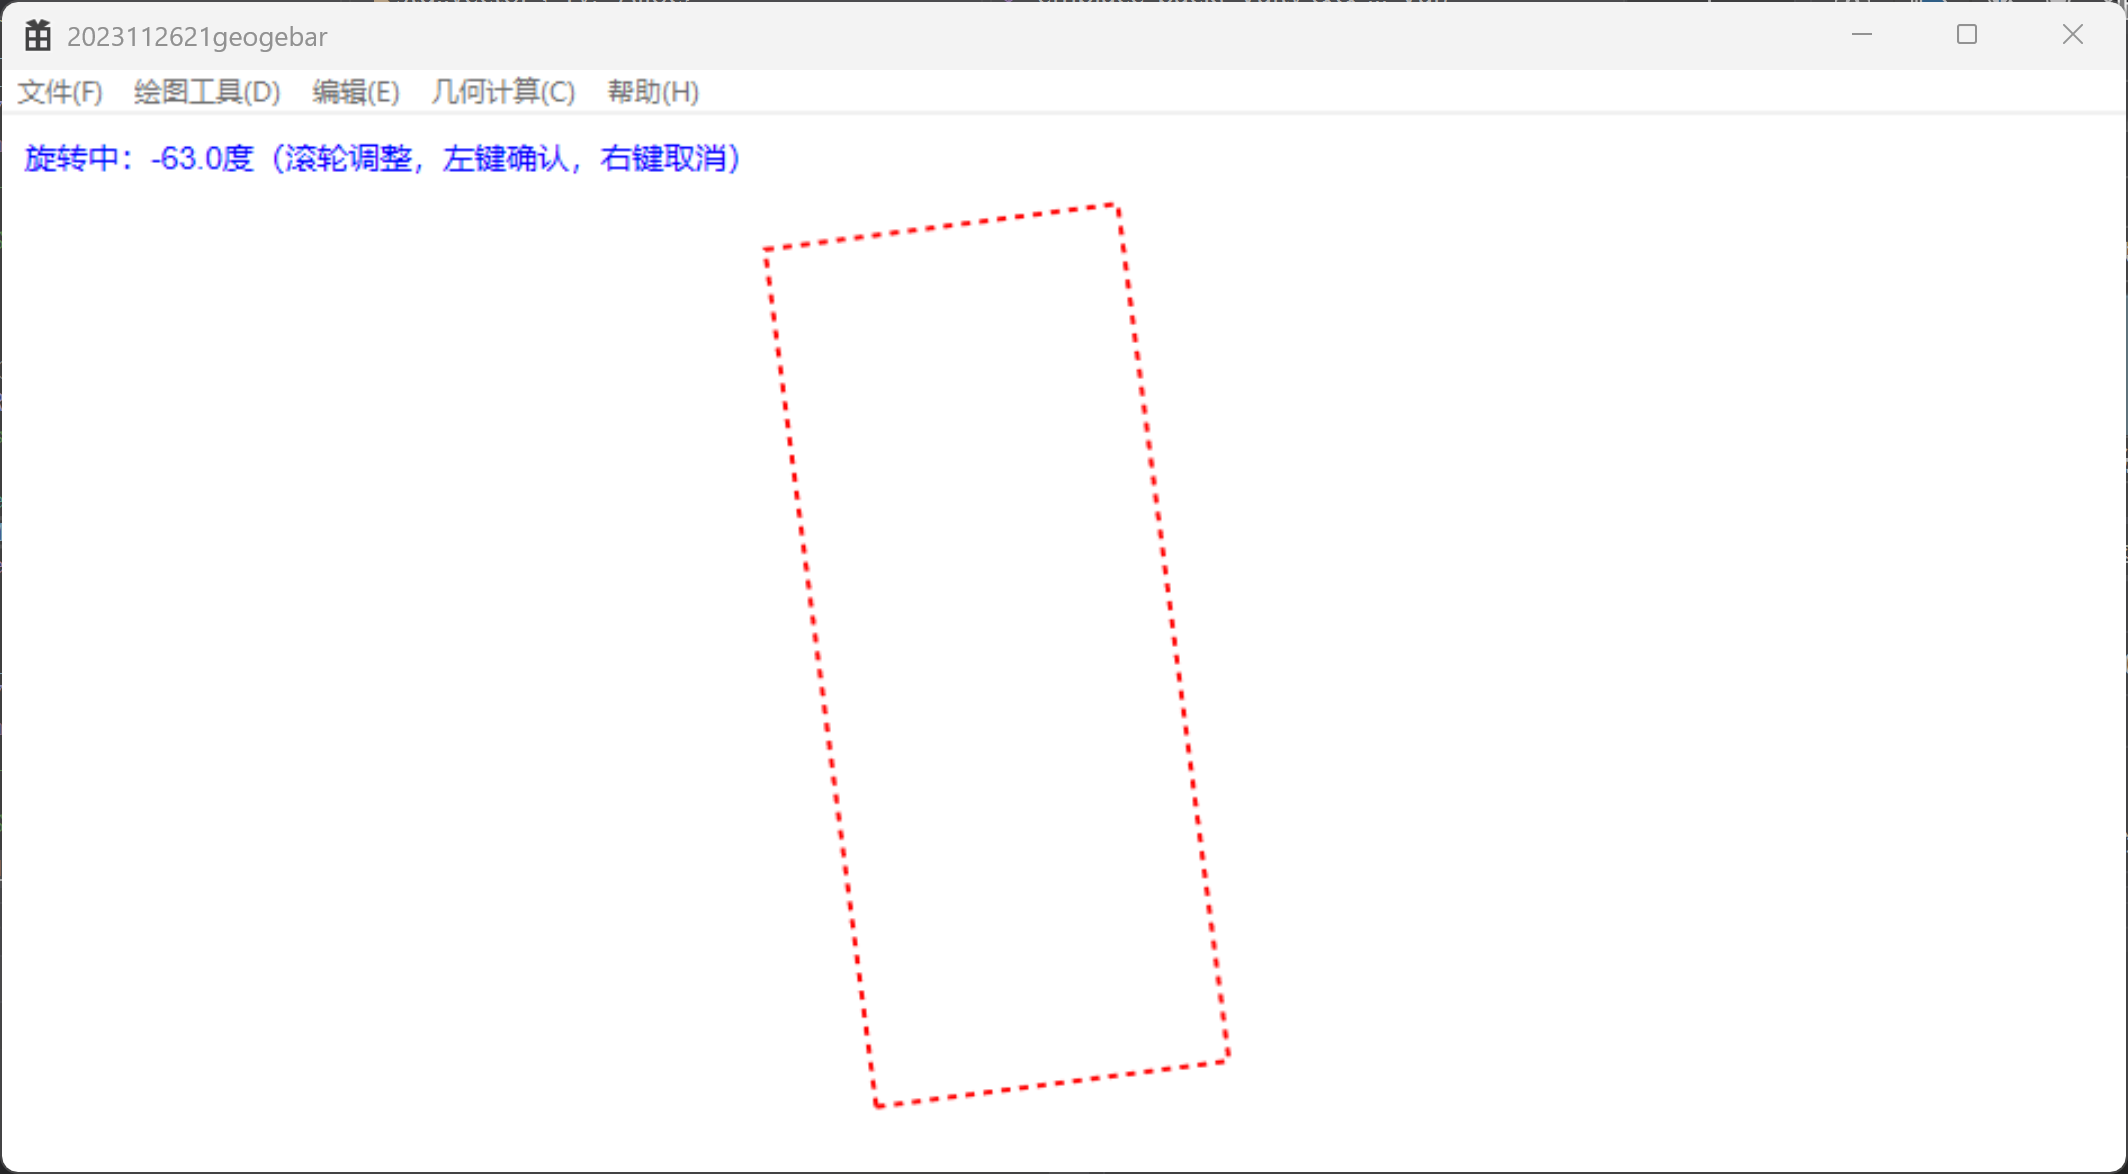
\includegraphics[width=0.92\textwidth]{images/xzfw1.png}
	\caption{右键取消旋转示例}
\end{figure}
\begin{figure}[H]
	\centering
	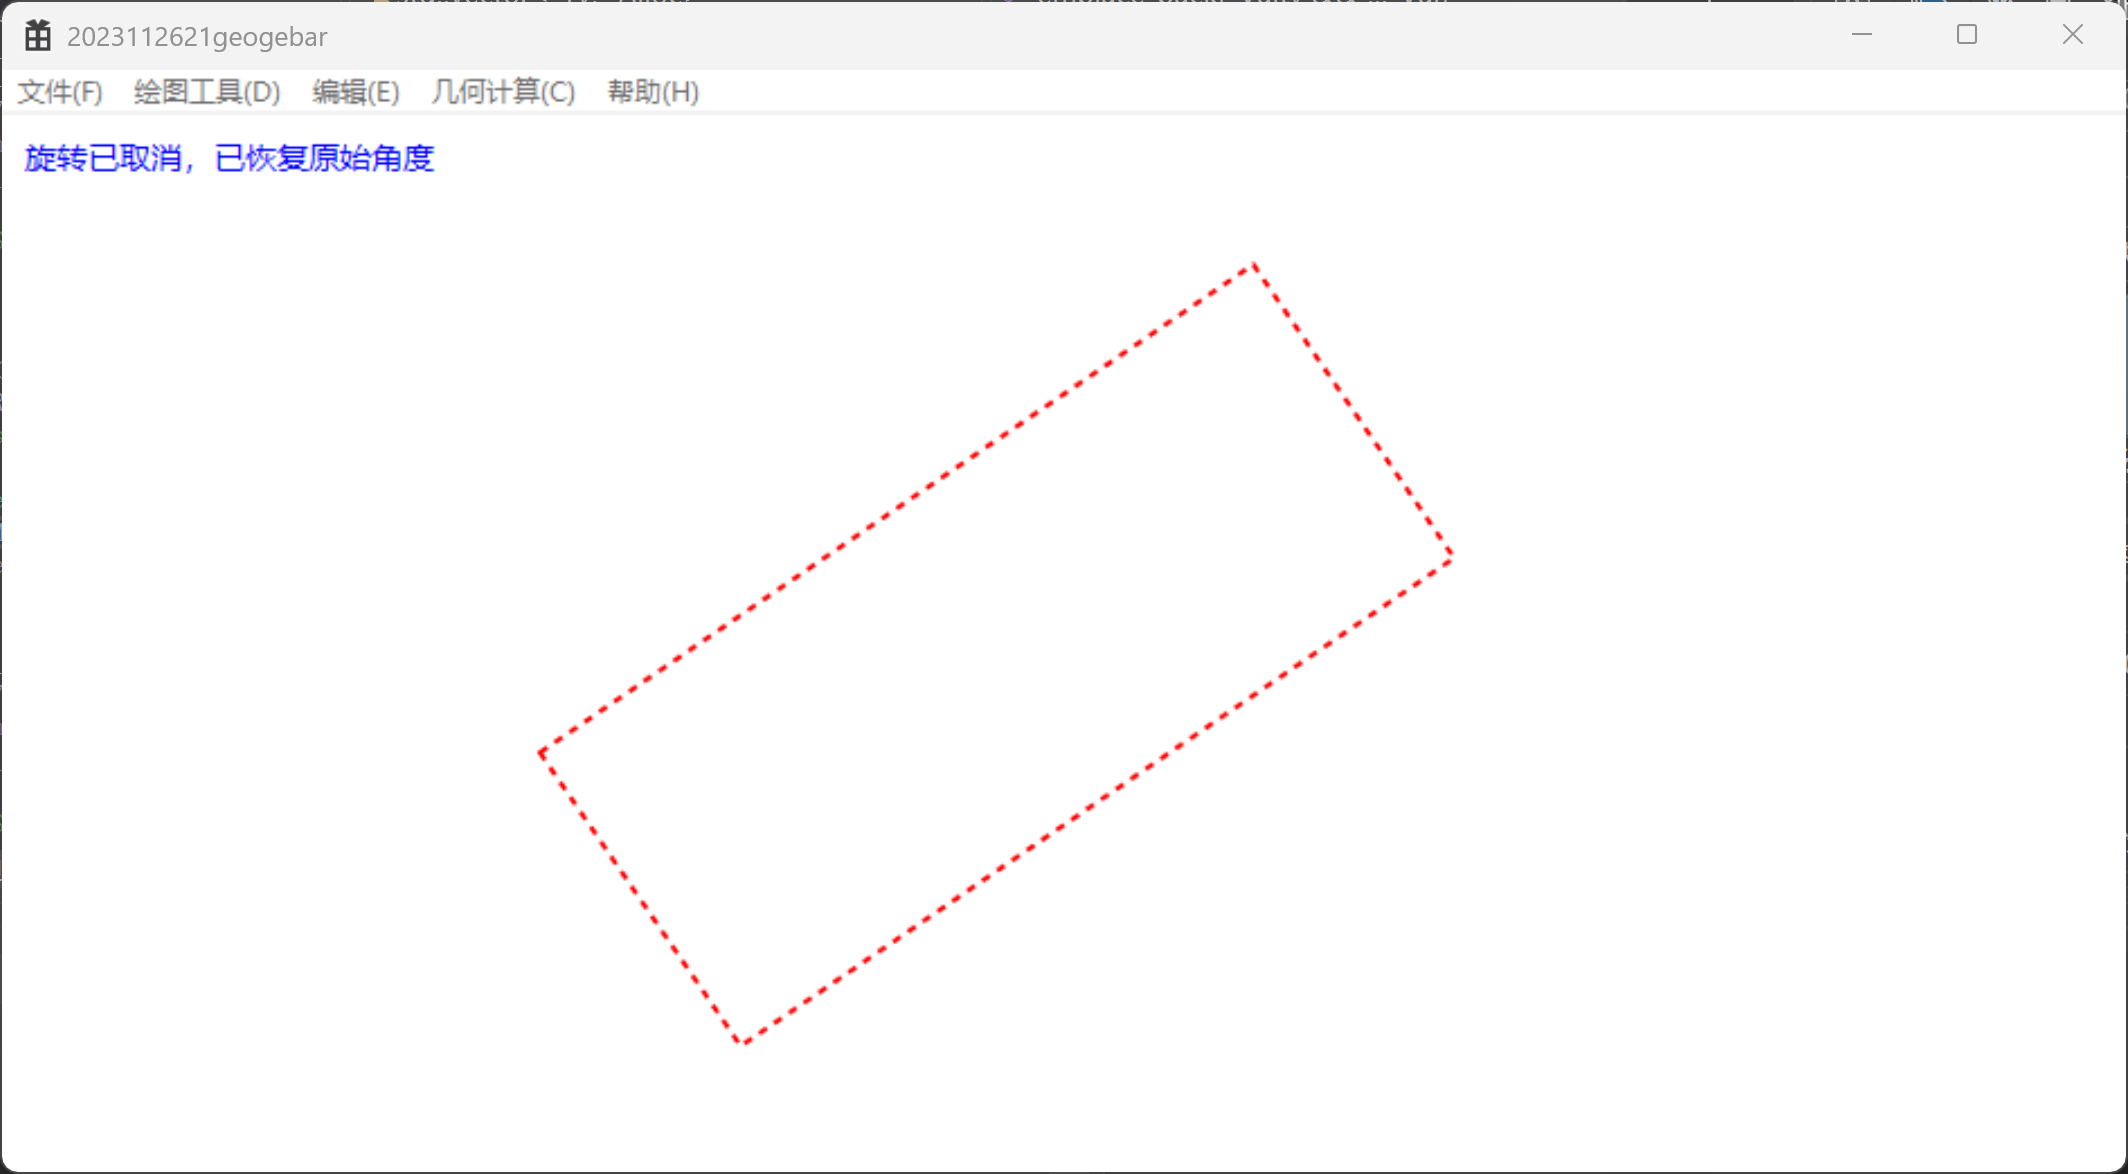
\includegraphics[width=0.92\textwidth]{images/xzfw2.png}
	\caption{右键取消旋转示例}
\end{figure}

\textbf{4. 缩放图形}
\begin{enumerate}
    \item 先选中要缩放的图形
    \item 点击菜单"编辑→缩放"
    \item 滚动鼠标滚轮调整缩放比例
    \begin{itemize}
        \item 向上滚动：放大（每次增加10\%）
        \item 向下滚动：缩小（每次减少10\%）
        \item 缩放范围：0.1倍到10倍
    \end{itemize}
    \item 缩放过程中可实时预览效果
    \item 点击鼠标左键确认缩放
    \item 点击鼠标右键取消缩放，恢复原状
\end{enumerate}

% 在此处插入缩放图形的截图
\begin{figure}[H]
	\centering
	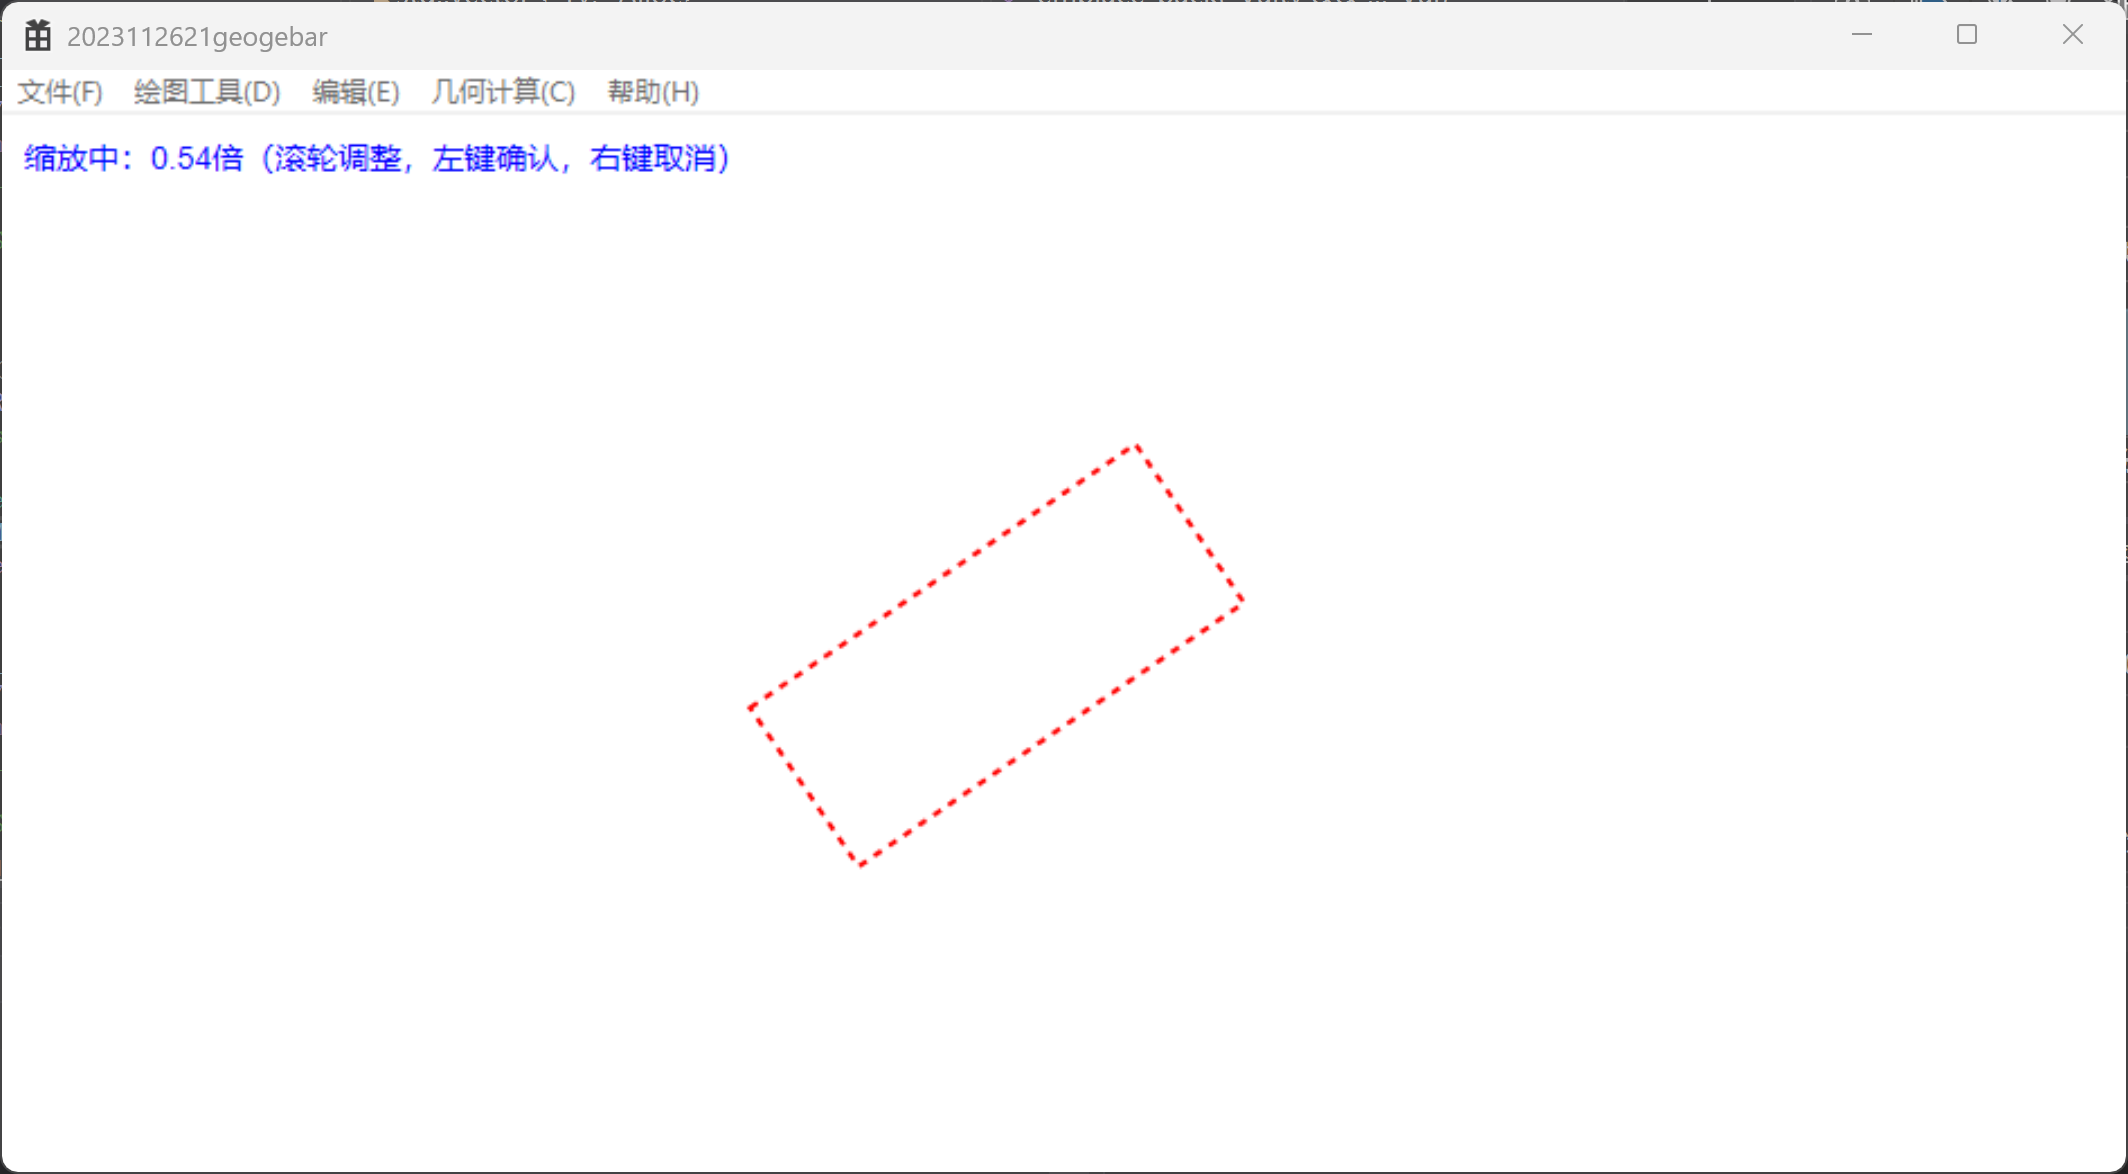
\includegraphics[width=0.92\textwidth]{images/sf1.png}
	\caption{缩放图形示例（缩小）}
\end{figure}
\begin{figure}[H]
	\centering
	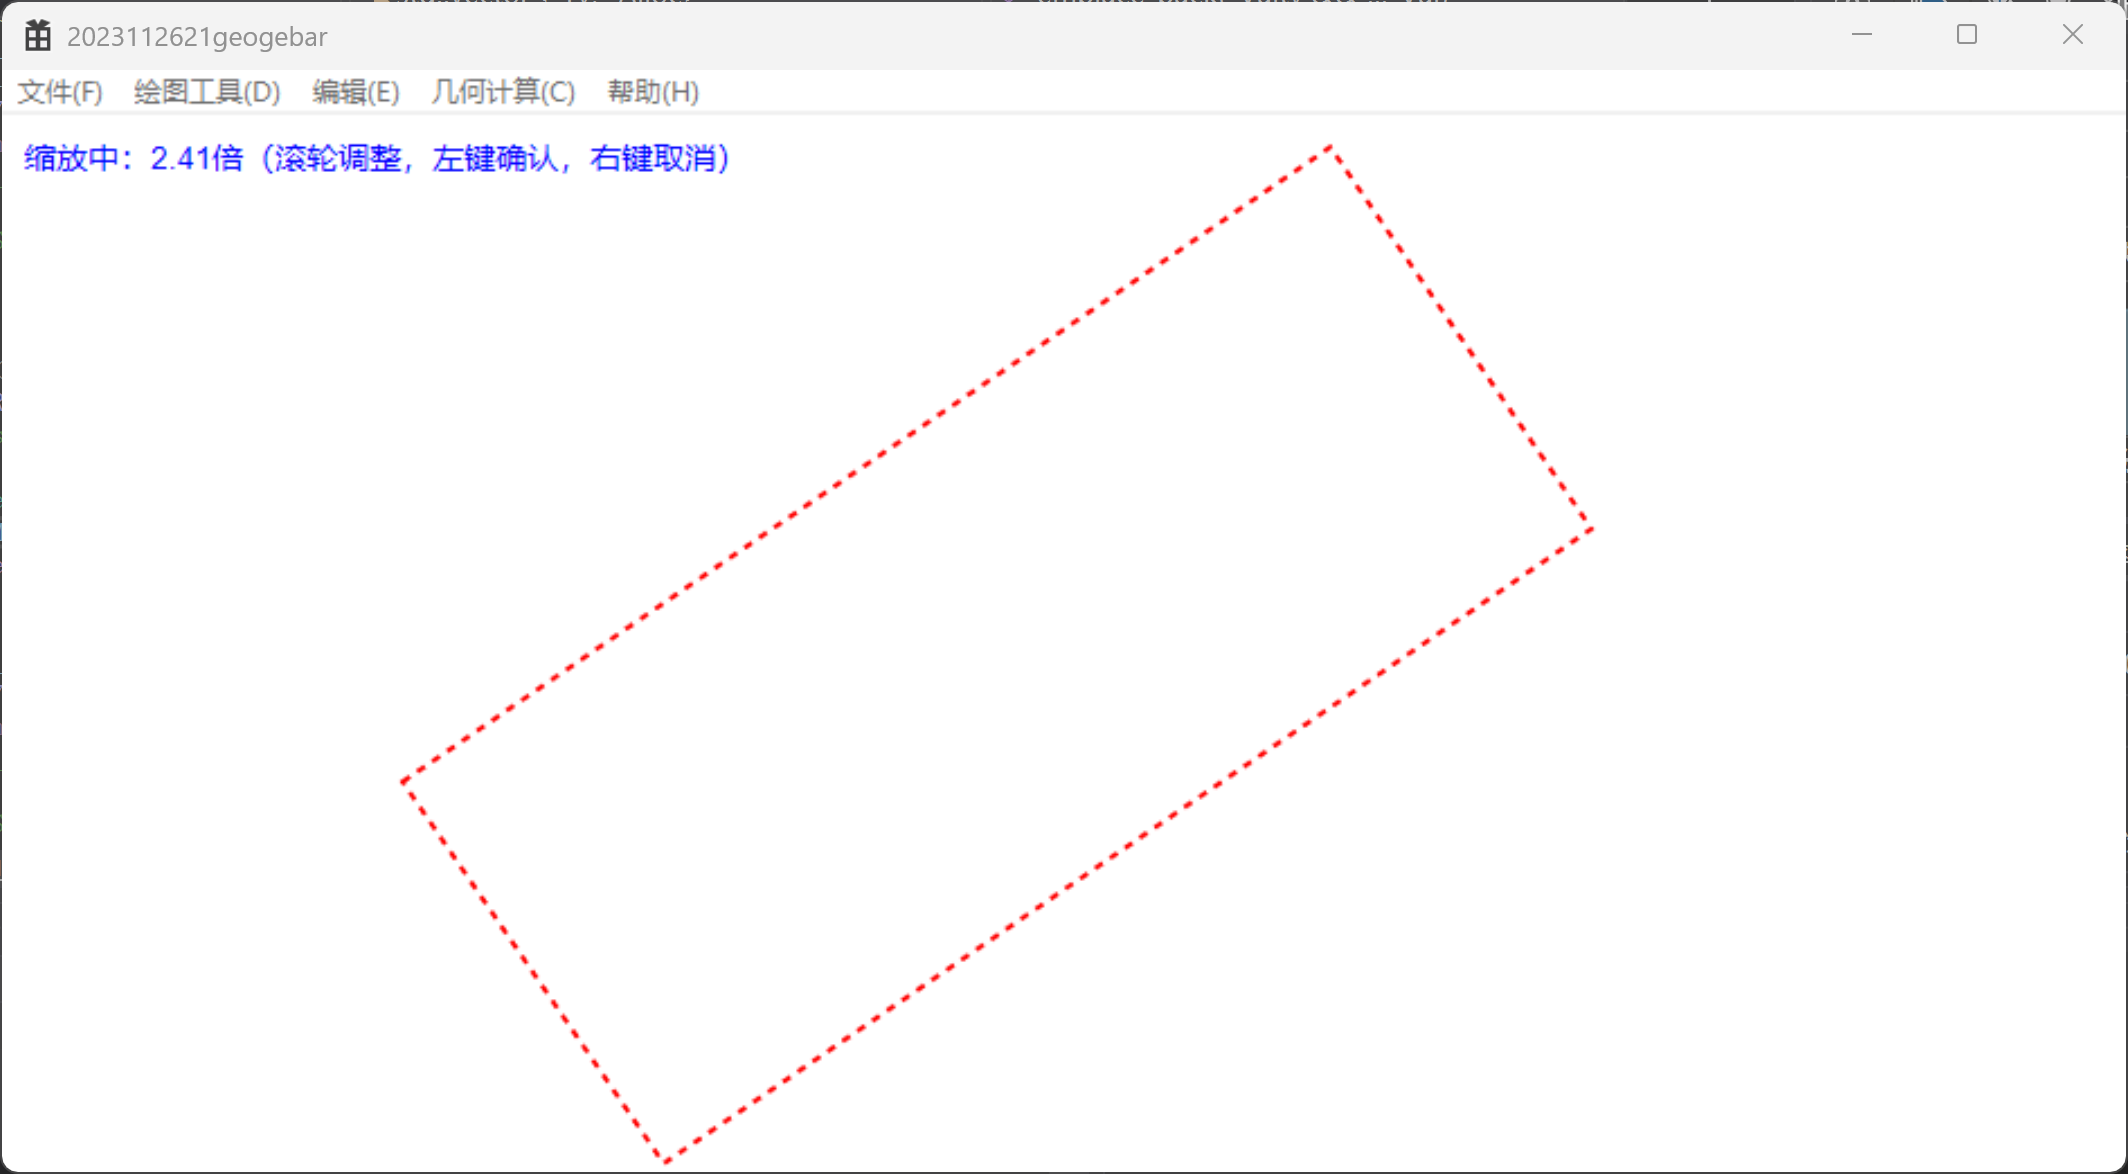
\includegraphics[width=0.92\textwidth]{images/sf2.png}
	\caption{缩放图形示例（放大）}
\end{figure}
\begin{figure}[H]
	\centering
	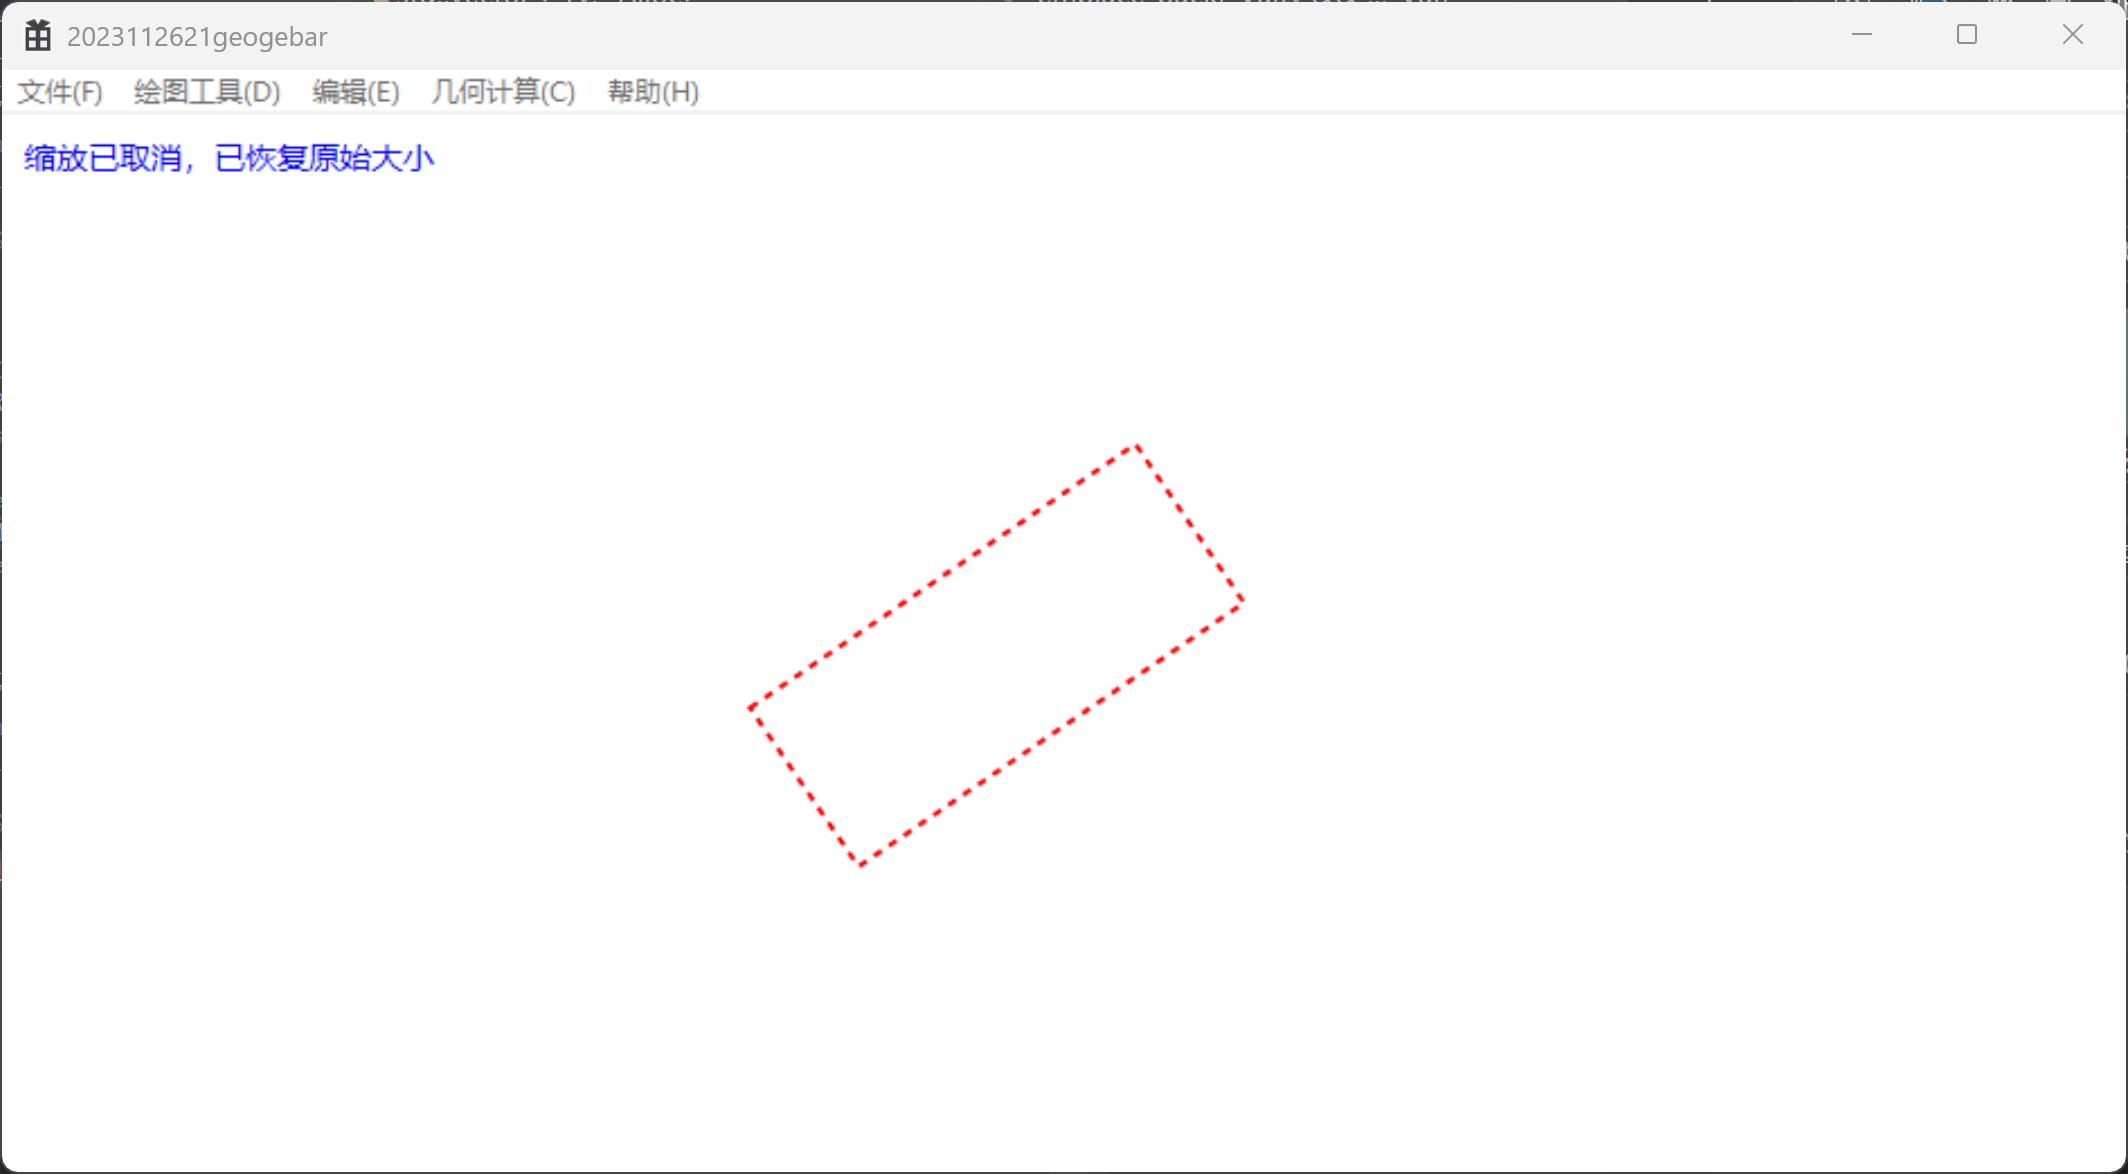
\includegraphics[width=0.92\textwidth]{images/sf3.png}
	\caption{缩放图形示例（复原大小）}
\end{figure}
\begin{figure}[H]
	\centering
	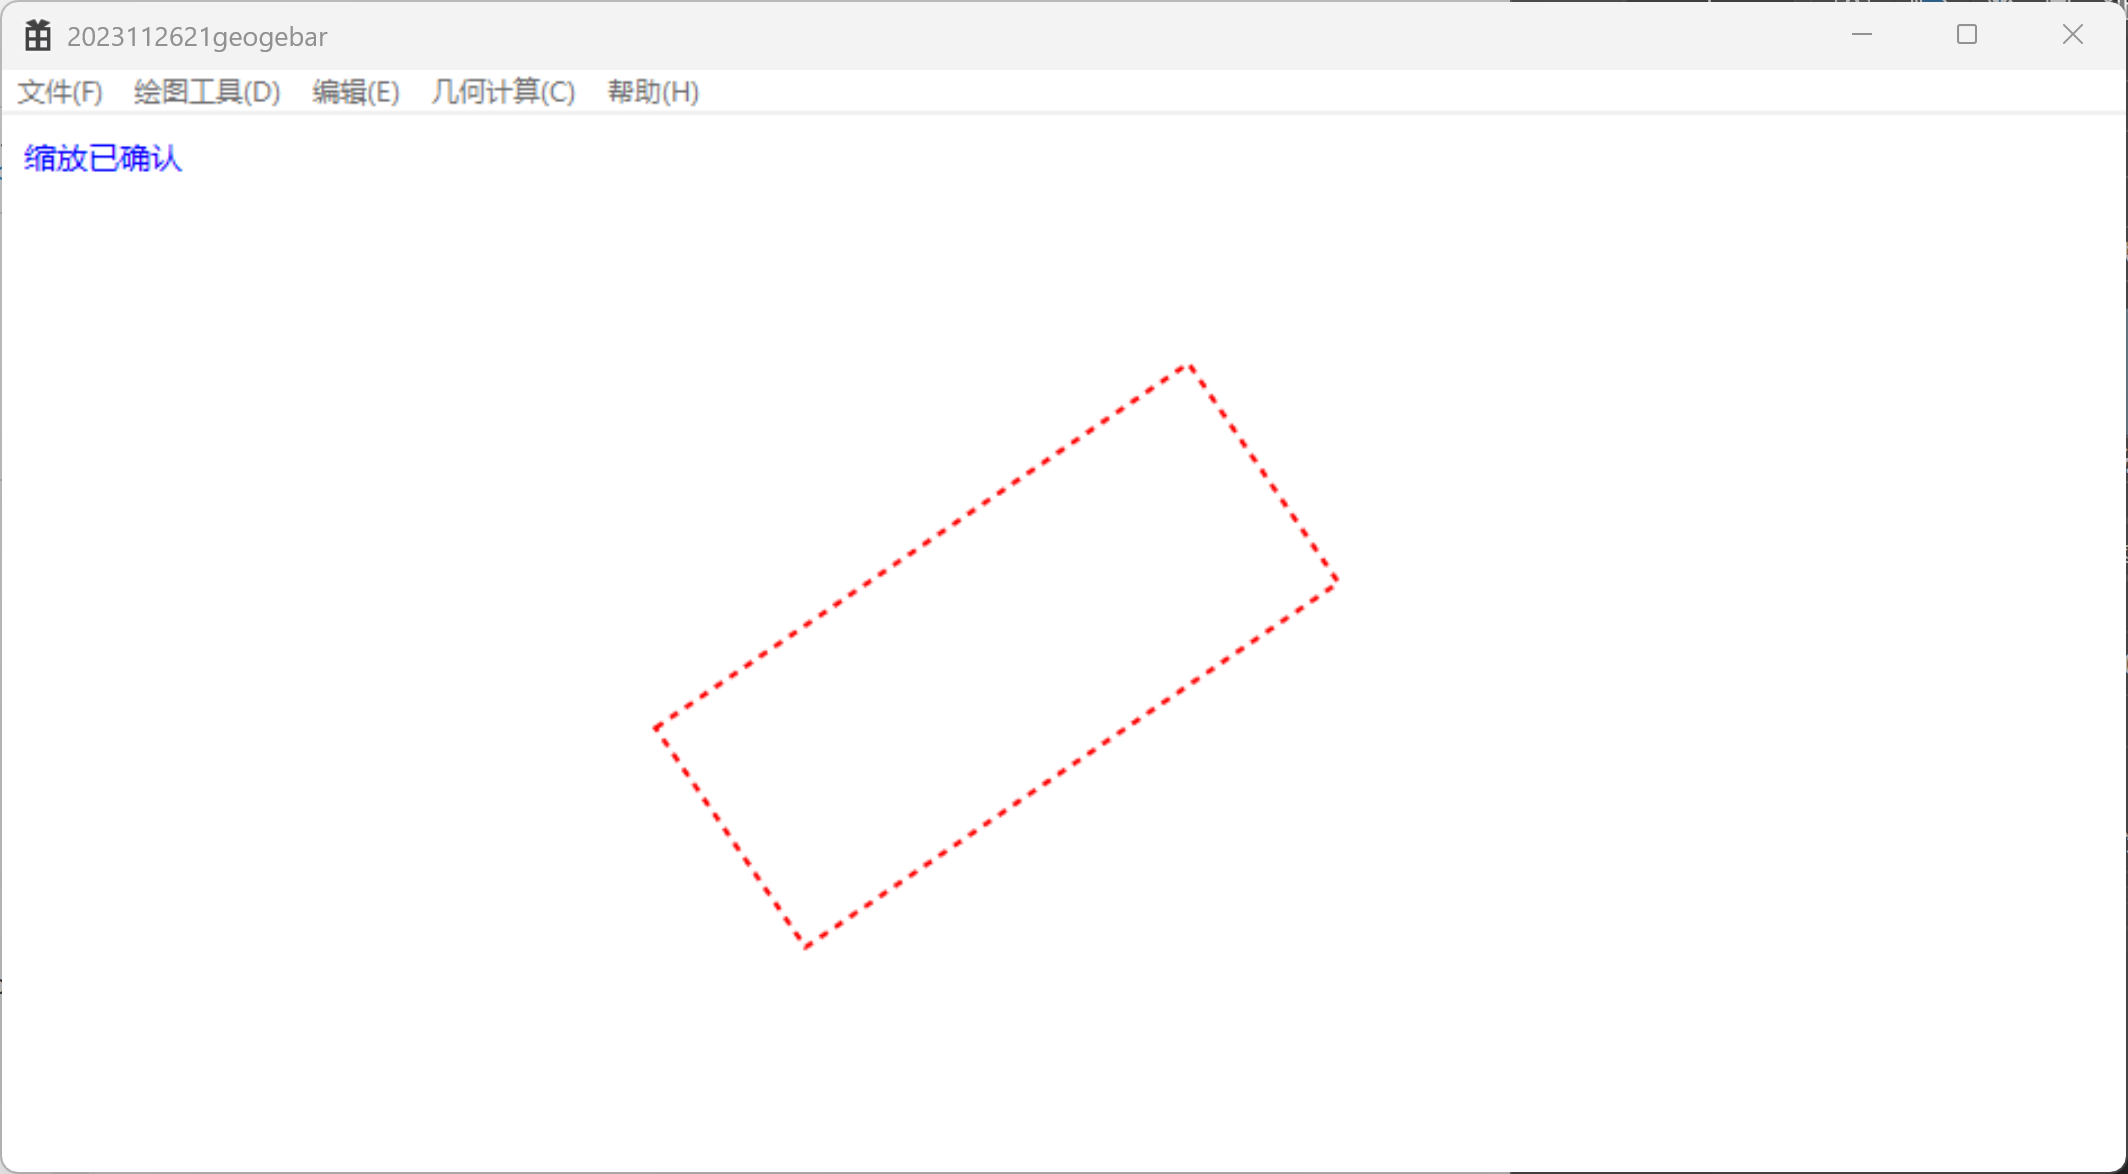
\includegraphics[width=0.92\textwidth]{images/sf4.png}
	\caption{右键取消缩放示例（确认缩放）}
\end{figure}

\textbf{5. 删除图形}
\begin{enumerate}
    \item 先选中要删除的图形
    \item 点击菜单"编辑→删除"或按Delete键
    \item 图形被删除（可通过撤销功能恢复）
\end{enumerate}

% 在此处插入删除图形的截图
\begin{figure}[H]
	\centering
	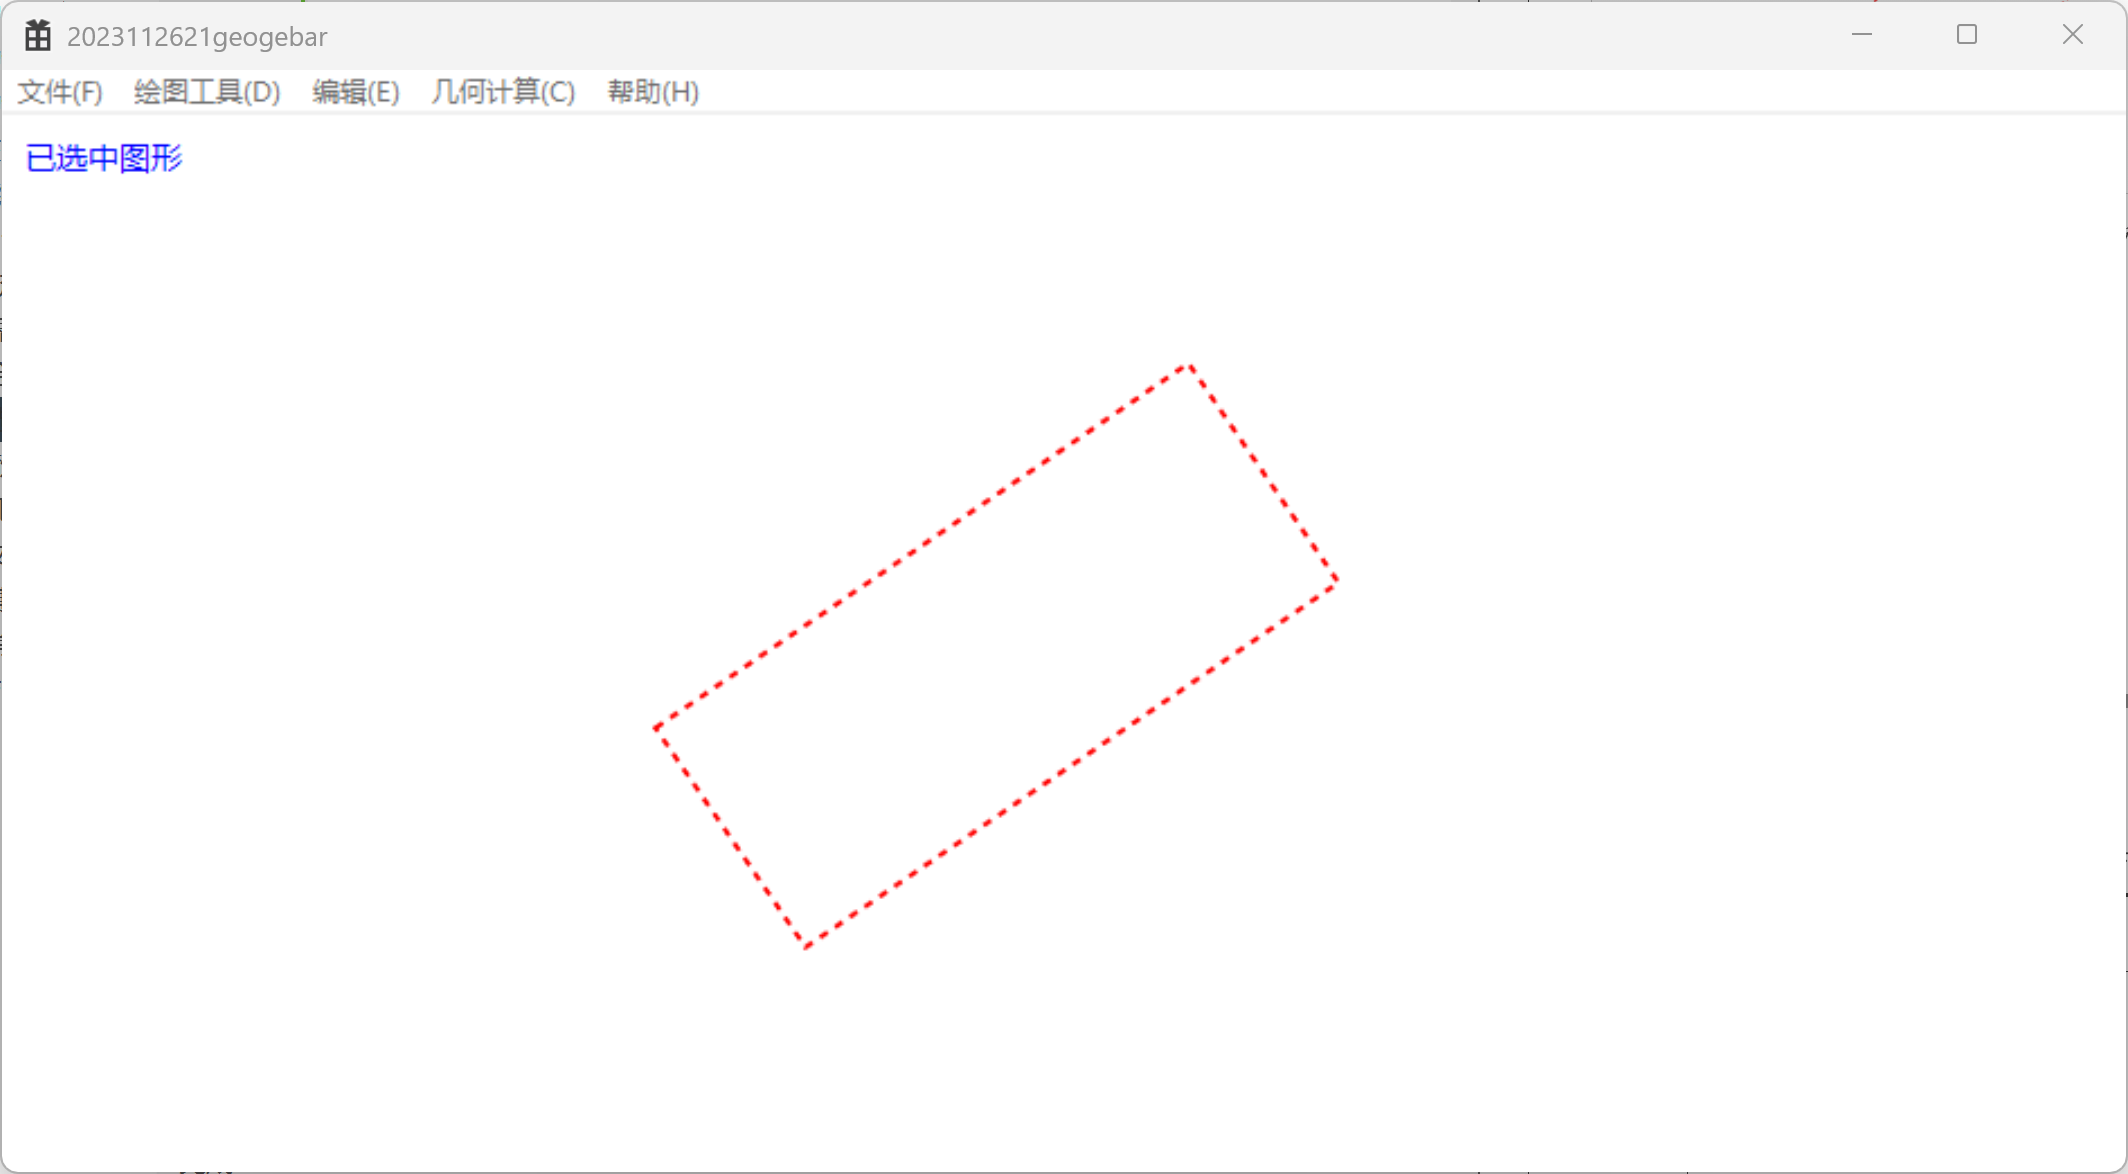
\includegraphics[width=0.92\textwidth]{images/sc1.png}
	\caption{删除图形示例（删除前）}
\end{figure}
\begin{figure}[H]
	\centering
	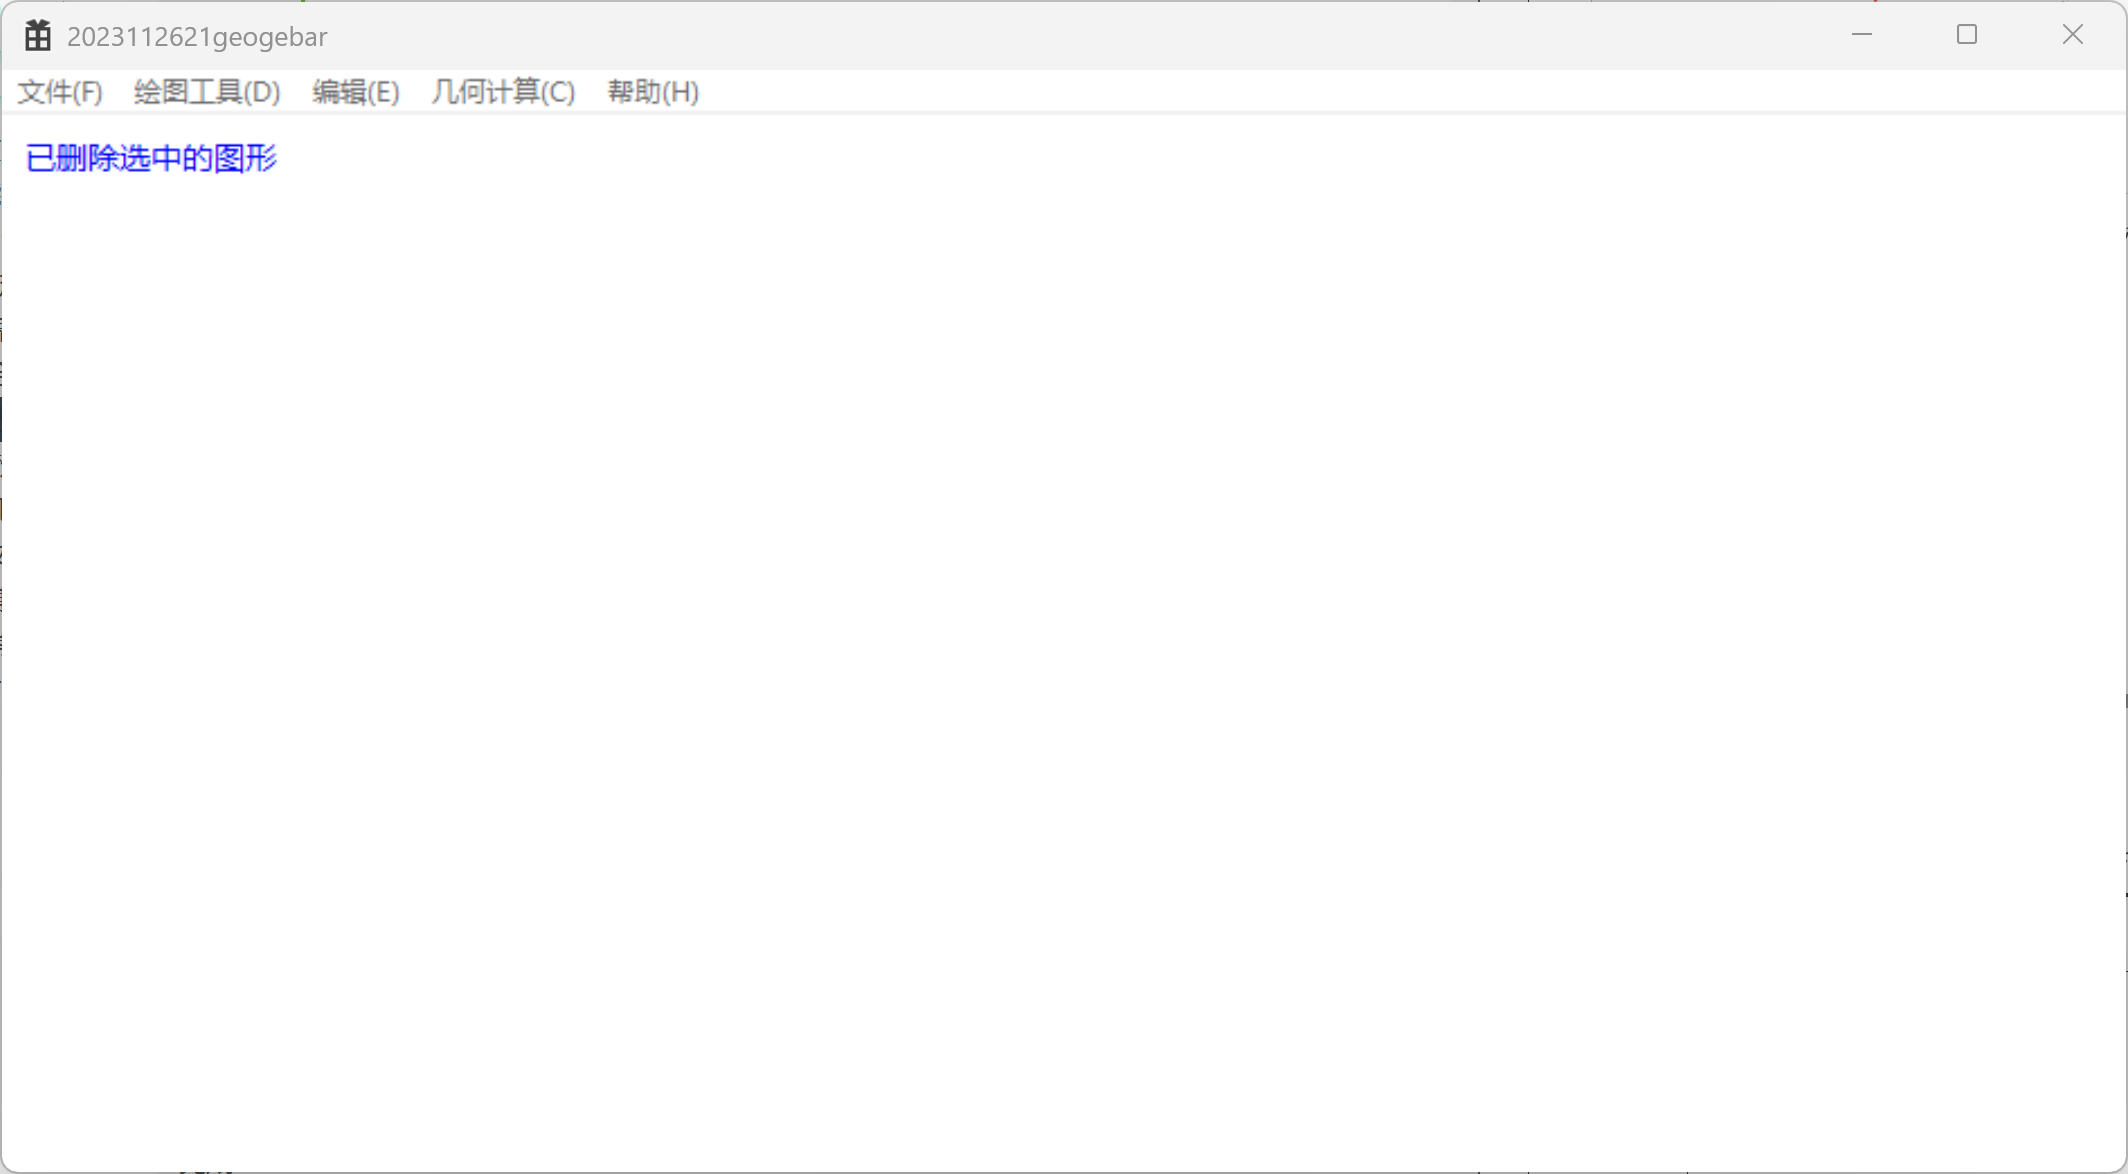
\includegraphics[width=0.92\textwidth]{images/sc2.png}
	\caption{删除图形示例（删除后）}
\end{figure}
\end{tcolorbox}

\subsection{撤销与重做操作}

\begin{tcolorbox}
\textbf{撤销操作}
\begin{enumerate}
    \item 点击菜单"编辑→撤销"或按快捷键Ctrl+Z
    \item 系统恢复到上一个操作状态
    \item 可连续撤销最多50步操作
    \item 当没有可撤销的操作时，菜单项显示为灰色
\end{enumerate}

\textbf{重做操作}
\begin{enumerate}
    \item 点击菜单"编辑→重做"或按快捷键Ctrl+Y
    \item 系统恢复到下一个操作状态
    \item 只能重做已撤销的操作
    \item 执行新操作后，重做历史会被清空
\end{enumerate}

% 在此处插入撤销重做的截图
\begin{figure}[H]
	\centering
	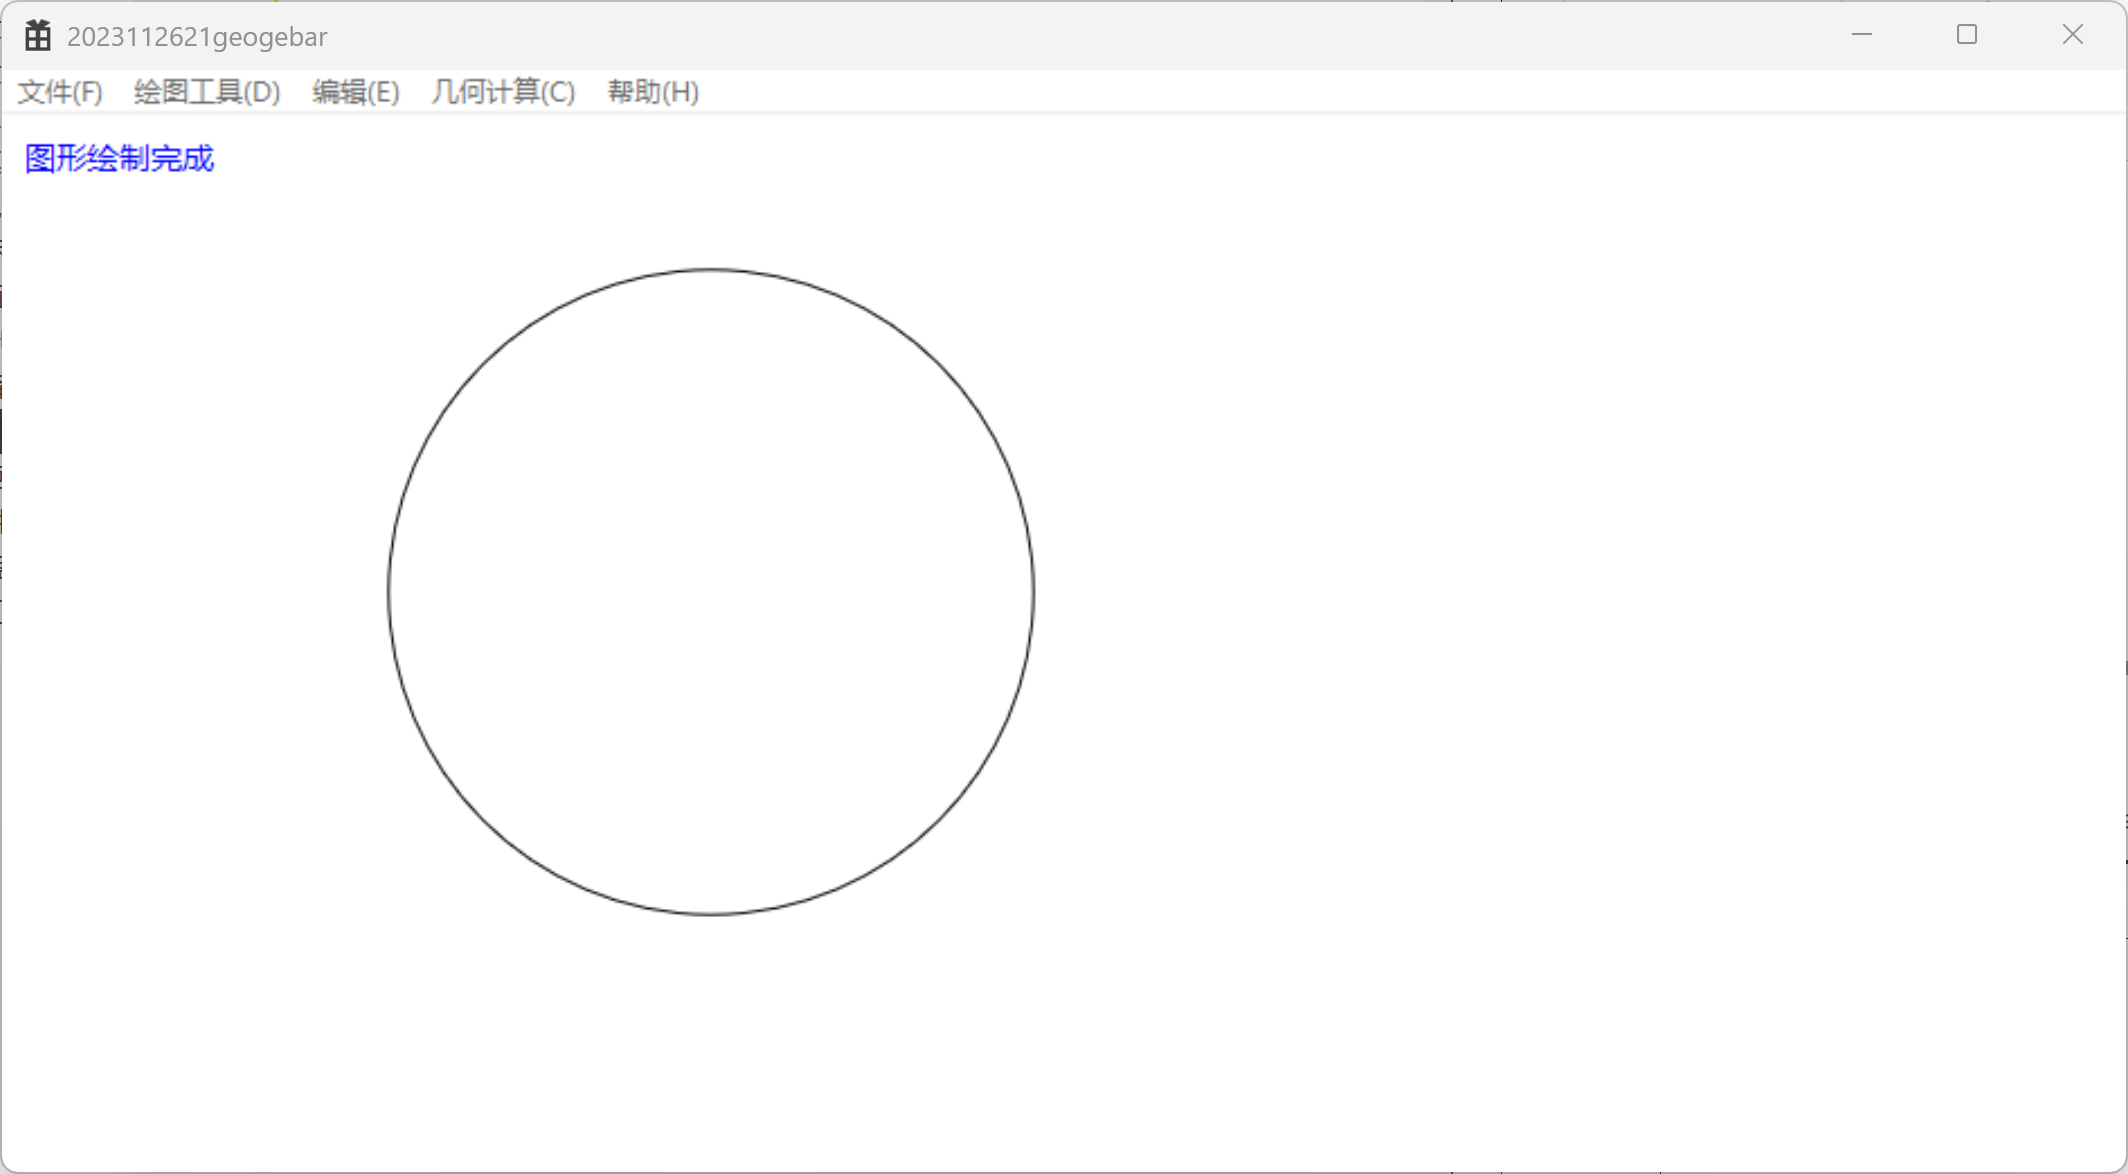
\includegraphics[width=0.92\textwidth]{images/chehui1.png}
	\caption{撤销操作示例（撤销前）}
\end{figure}
\begin{figure}[H]
	\centering
	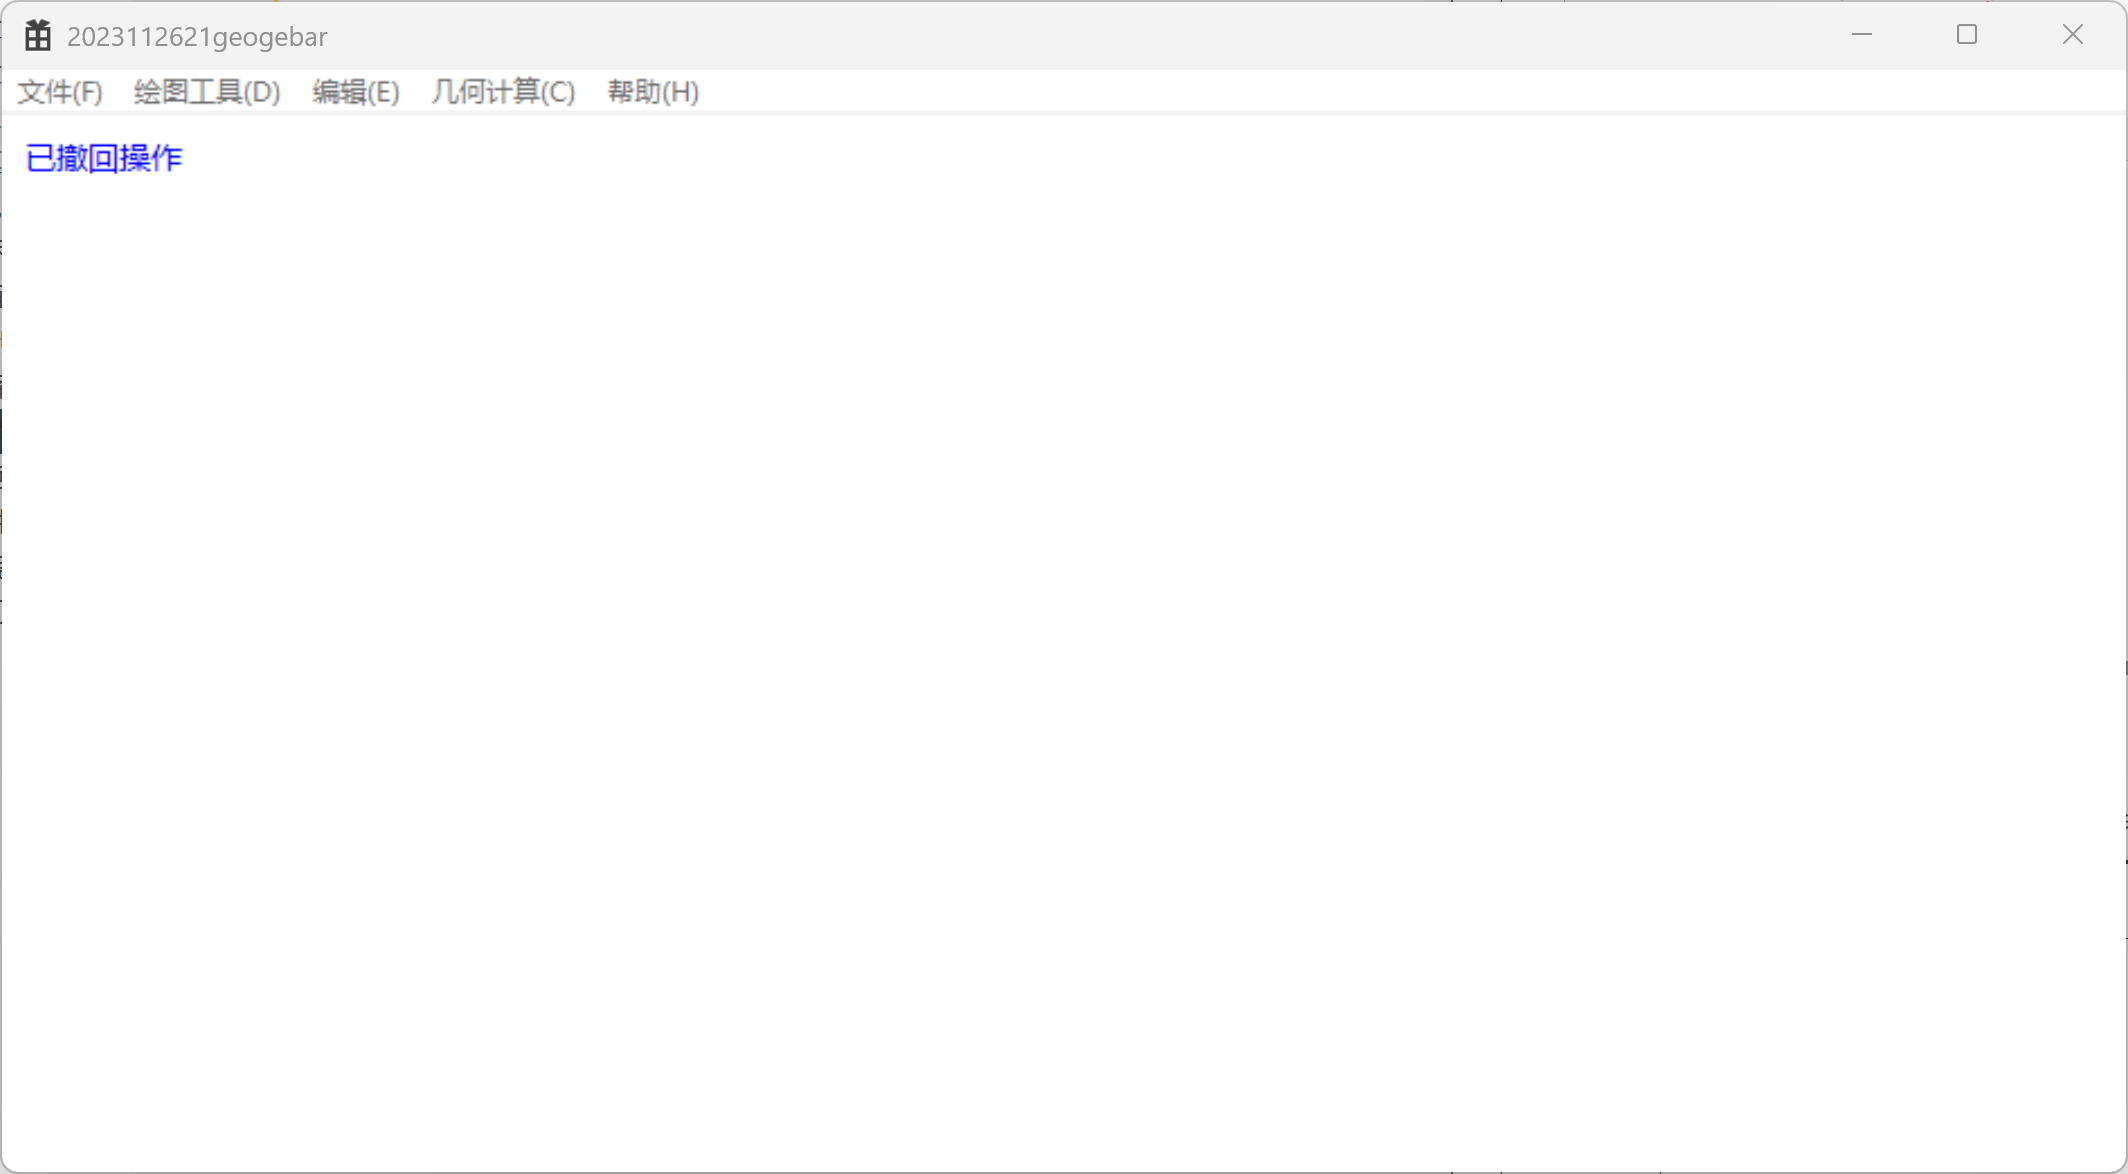
\includegraphics[width=0.92\textwidth]{images/chehui2.png}
	\caption{撤销操作示例（撤销后）}
\end{figure}
\begin{figure}[H]
	\centering
	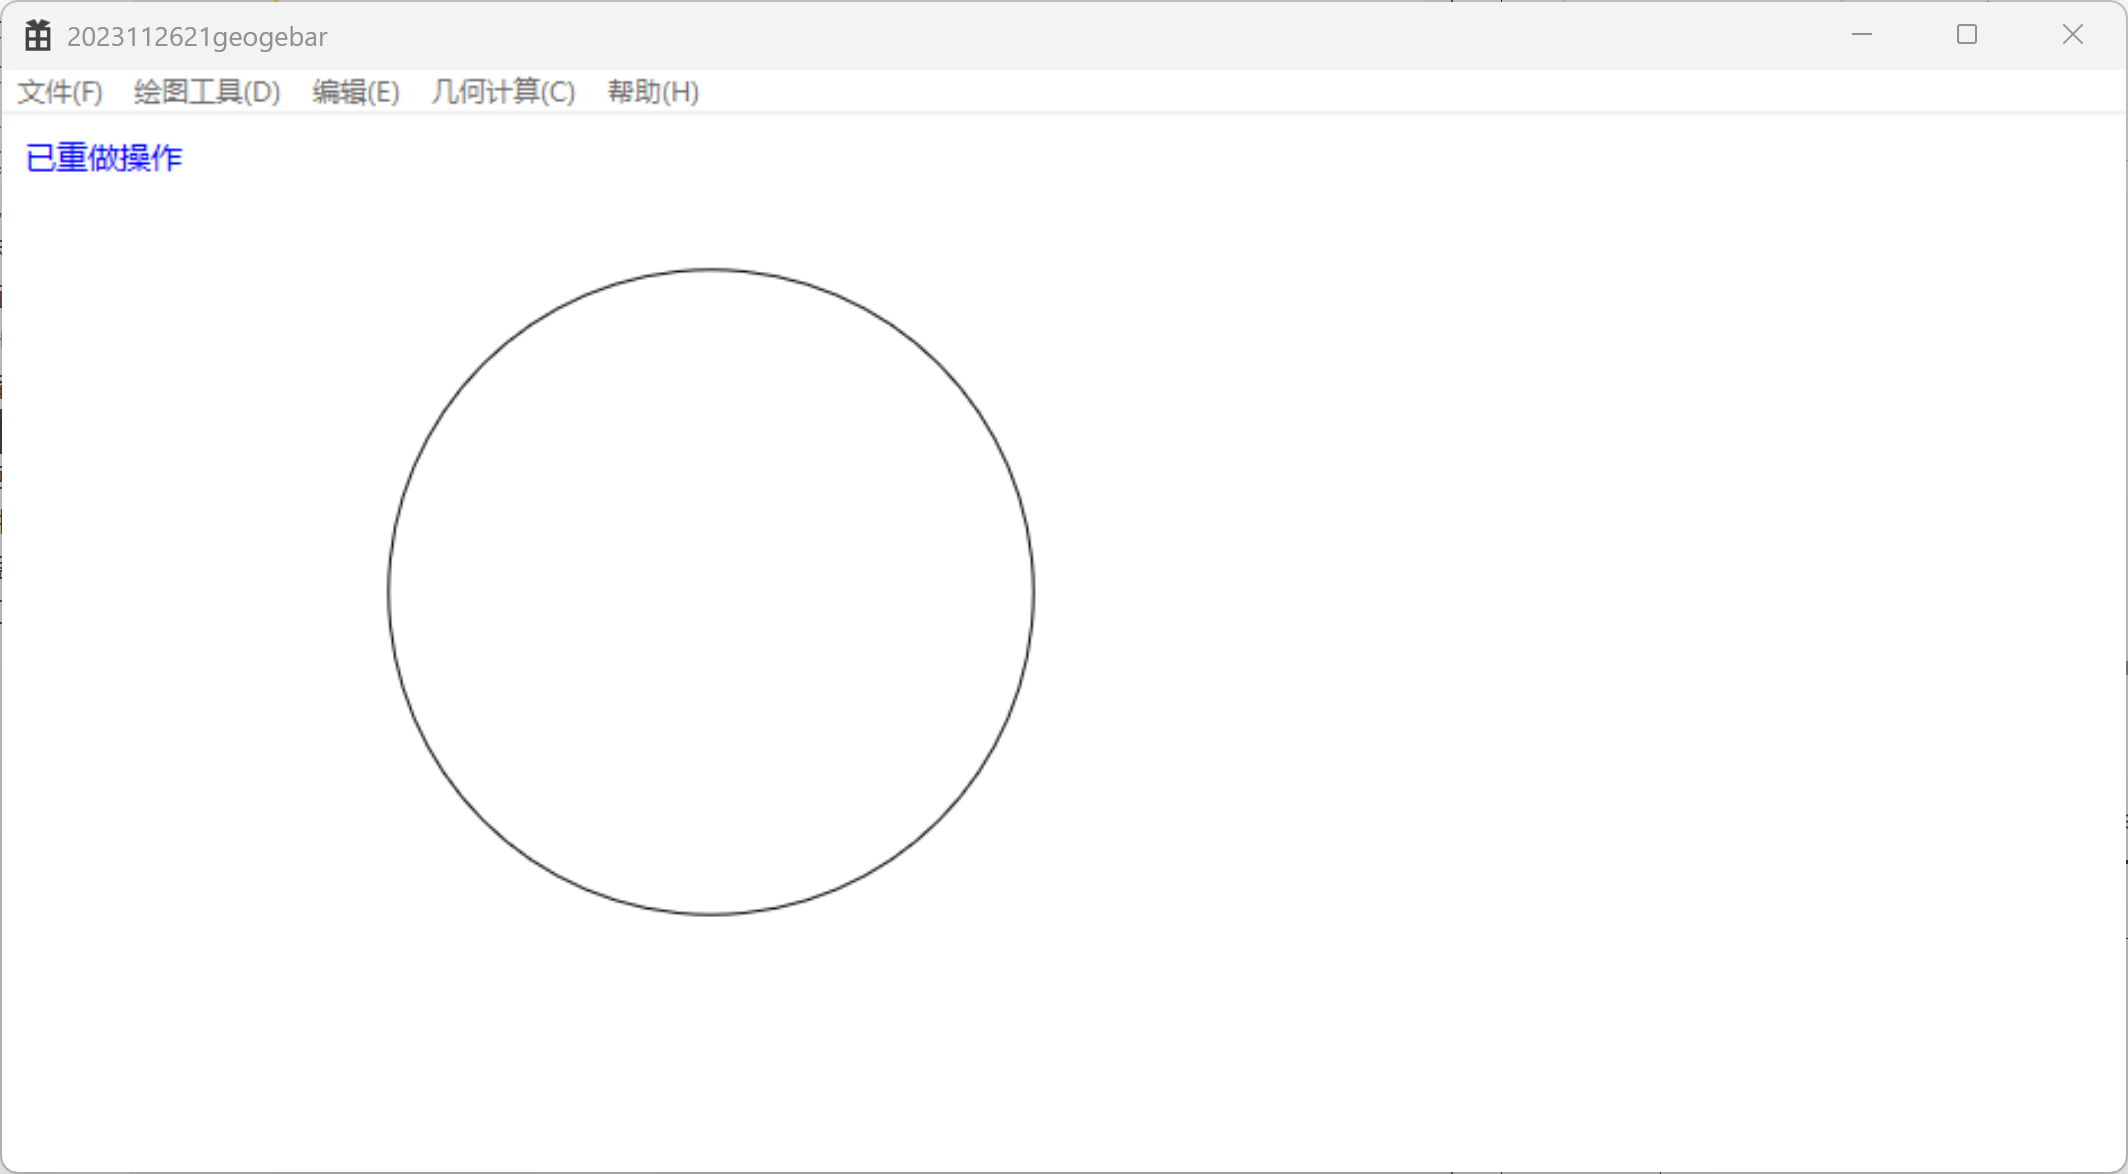
\includegraphics[width=0.92\textwidth]{images/chongzuo.png}
	\caption{重做操作示例}
\end{figure}
\end{tcolorbox}

\subsection{几何计算功能}

\begin{tcolorbox}
\textbf{1. 求交点}
\begin{enumerate}
    \item 点击菜单"计算→求交"
    \item 点击第一个图形（用蓝色高亮显示）
    \item 点击第二个图形（用绿色高亮显示）
    \item 系统自动计算并显示交点
    \item 交点用红色圆点标记
    \item 在消息框中显示交点坐标
\end{enumerate}

\textbf{支持的图形组合：}
\begin{itemize}
    \item 直线与直线：最多1个交点
    \item 直线与圆：最多2个交点
    \item 圆与圆：最多2个交点
\end{itemize}

% 在此处插入求交点的截图
\begin{figure}[H]
	\centering
	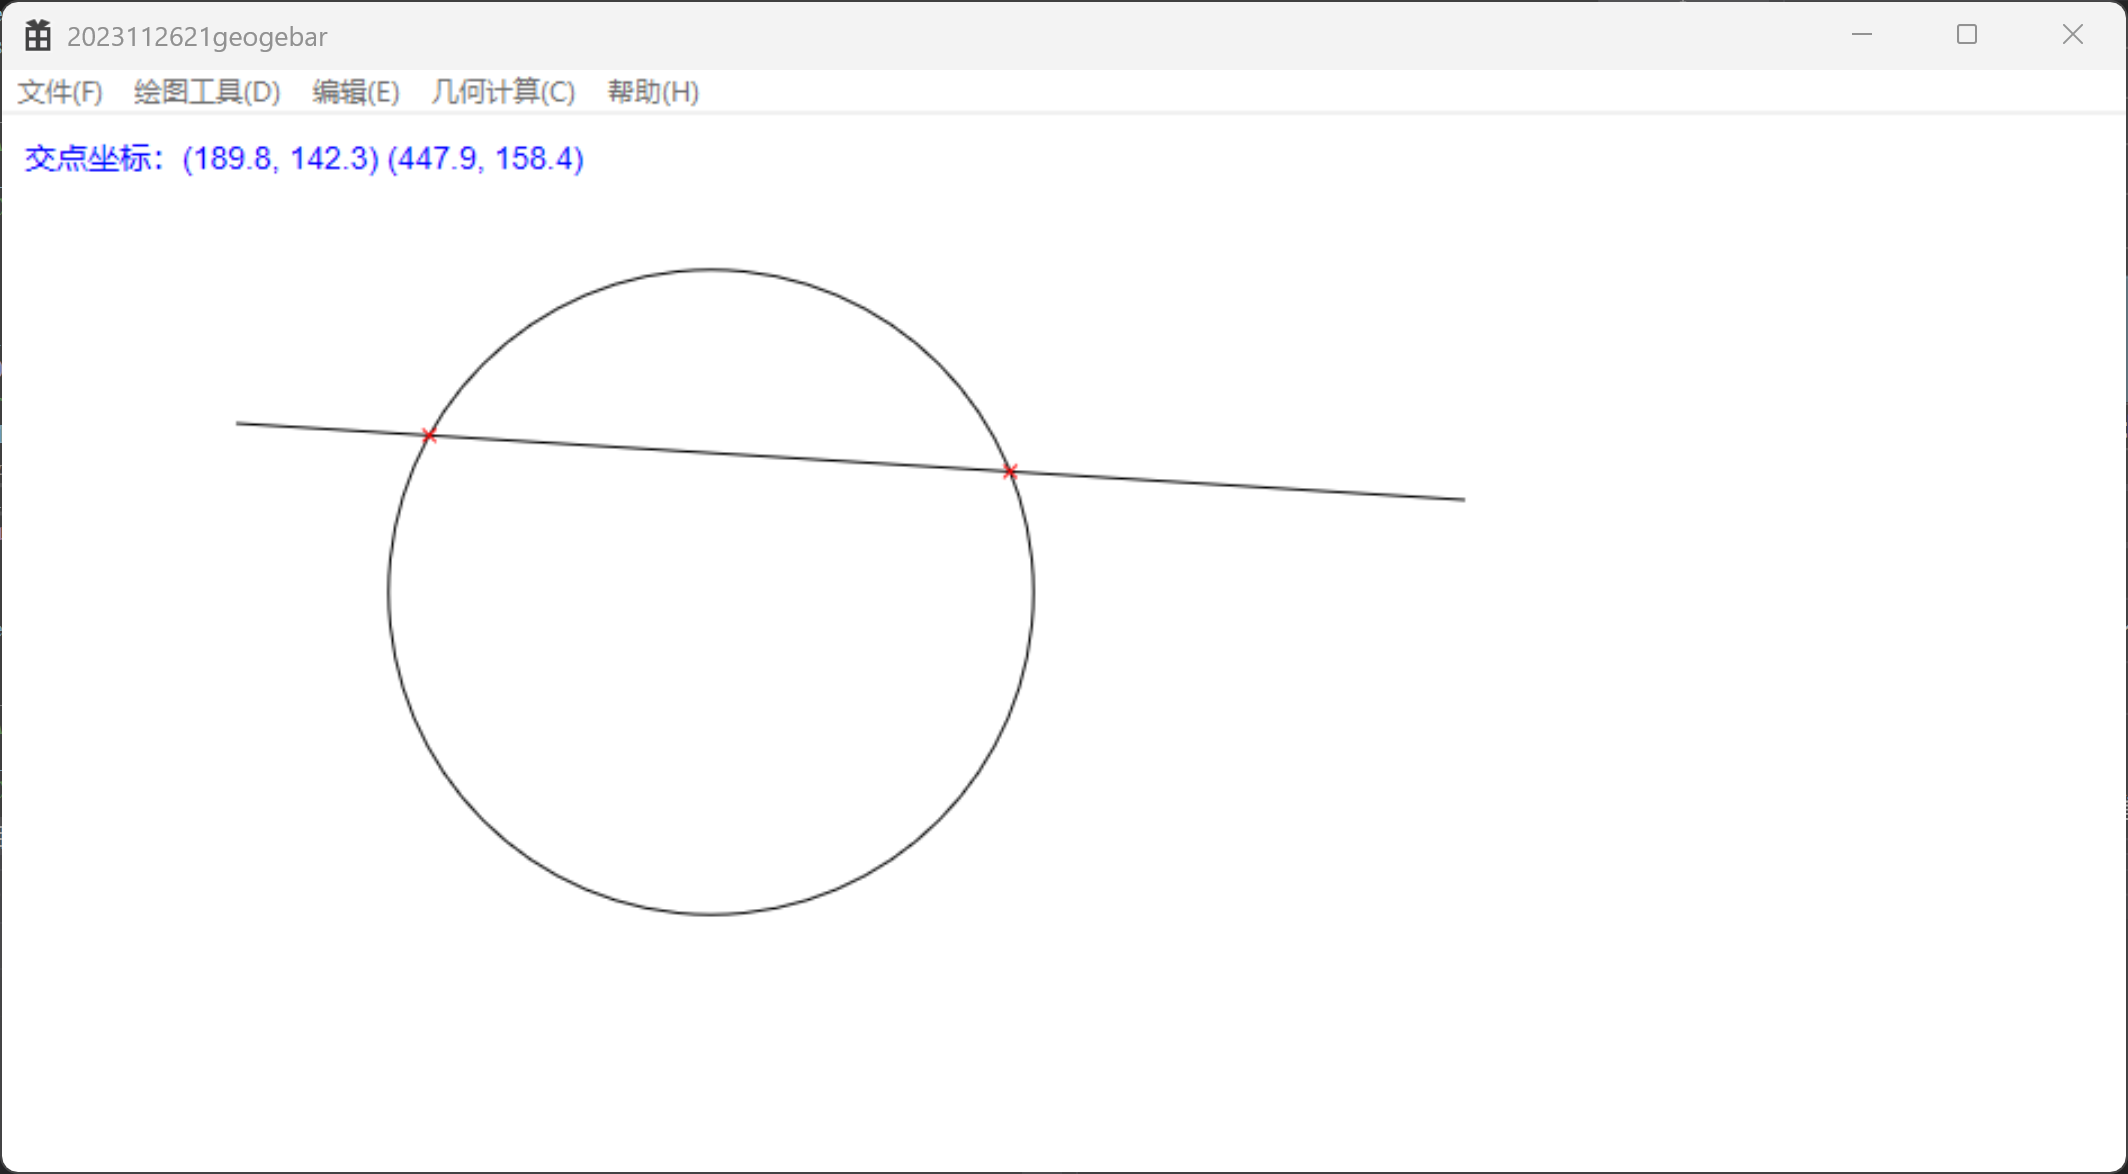
\includegraphics[width=0.92\textwidth]{images/qiujiao1.png}
	\caption{求交点示例}
\end{figure}
\begin{figure}[H]
	\centering
	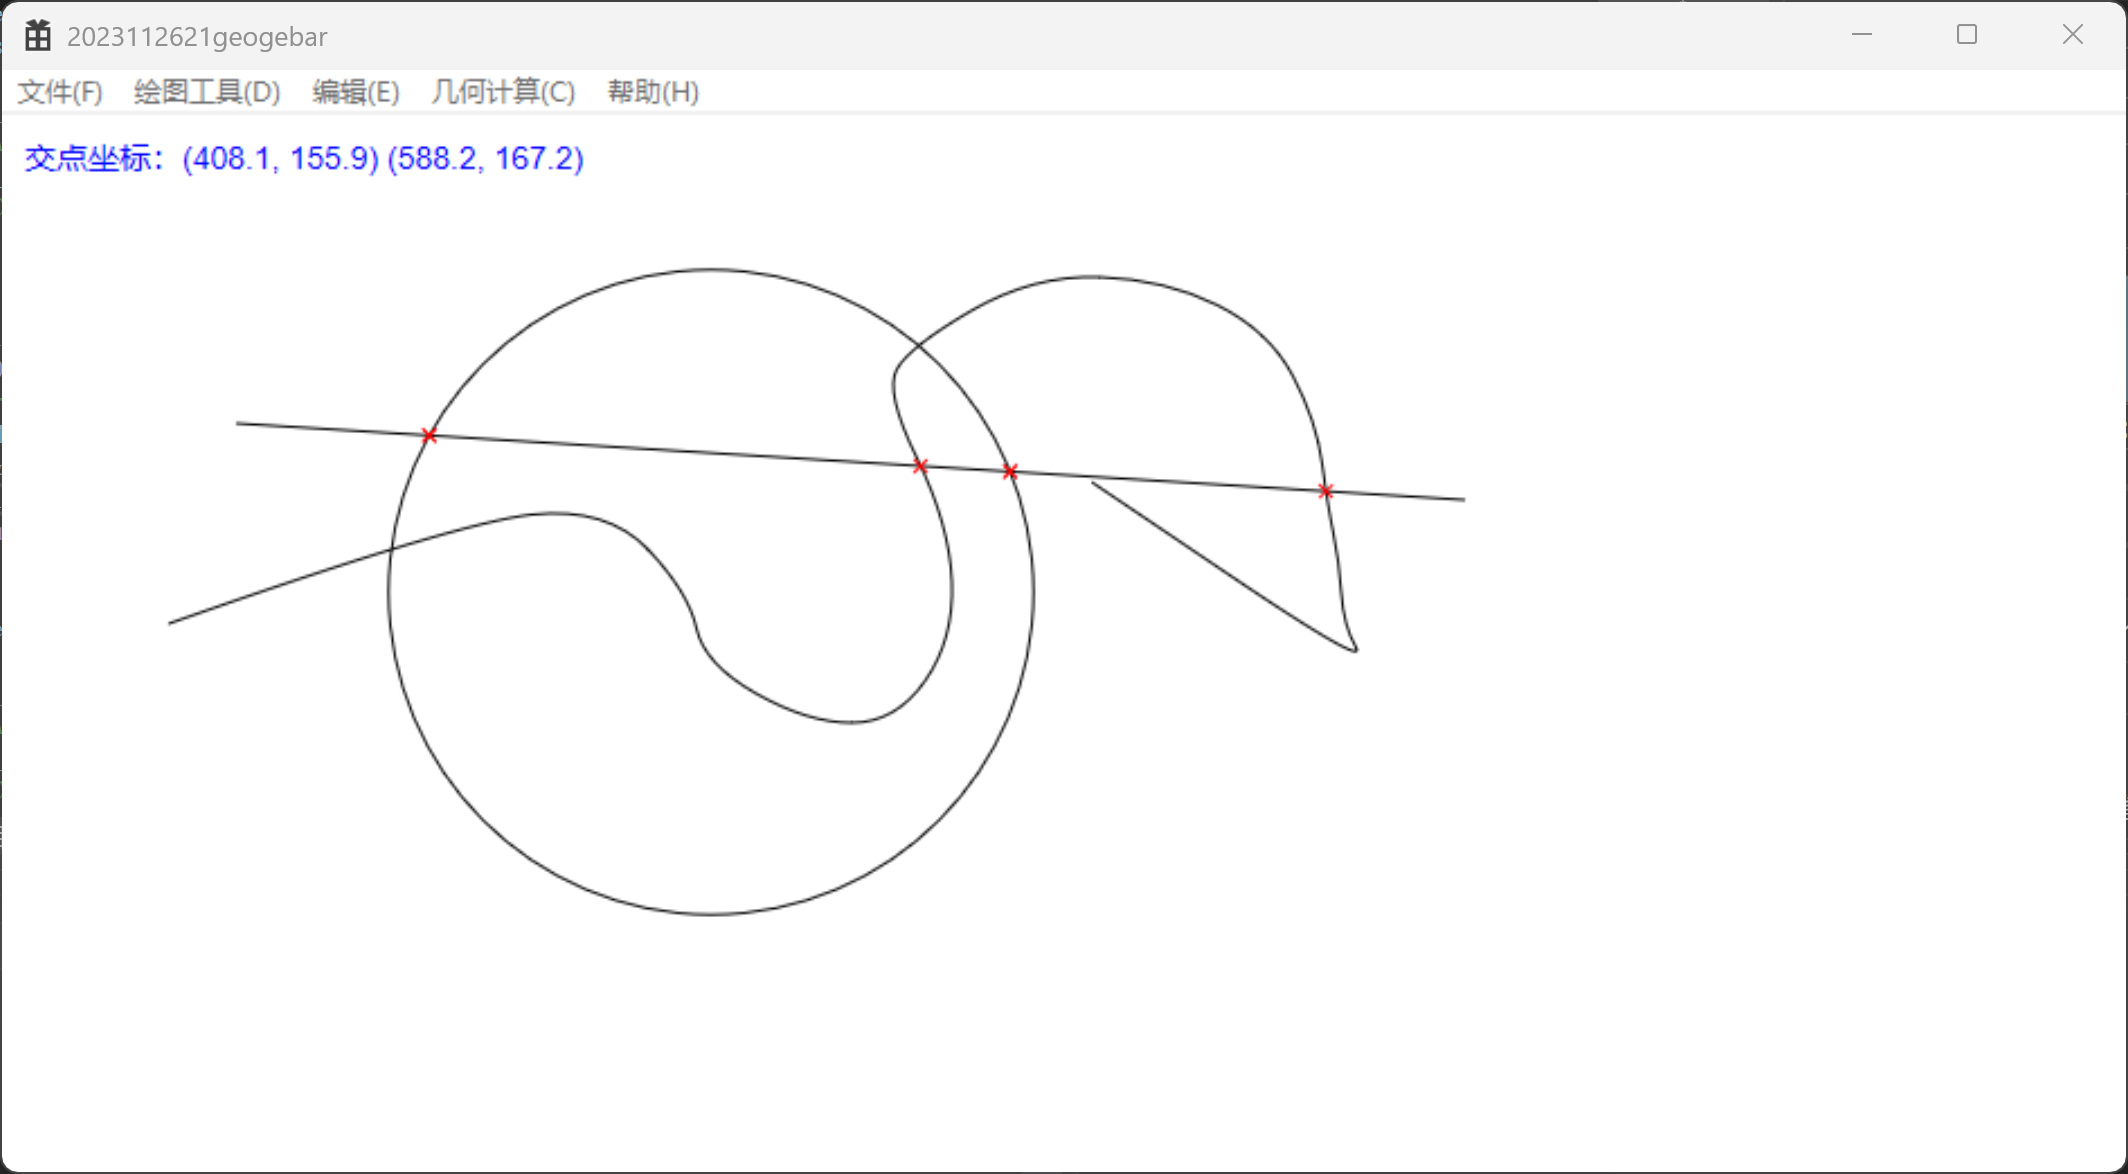
\includegraphics[width=0.92\textwidth]{images/qiujiao2.png}
	\caption{求交点示例}
\end{figure}
\begin{figure}[H]
	\centering
	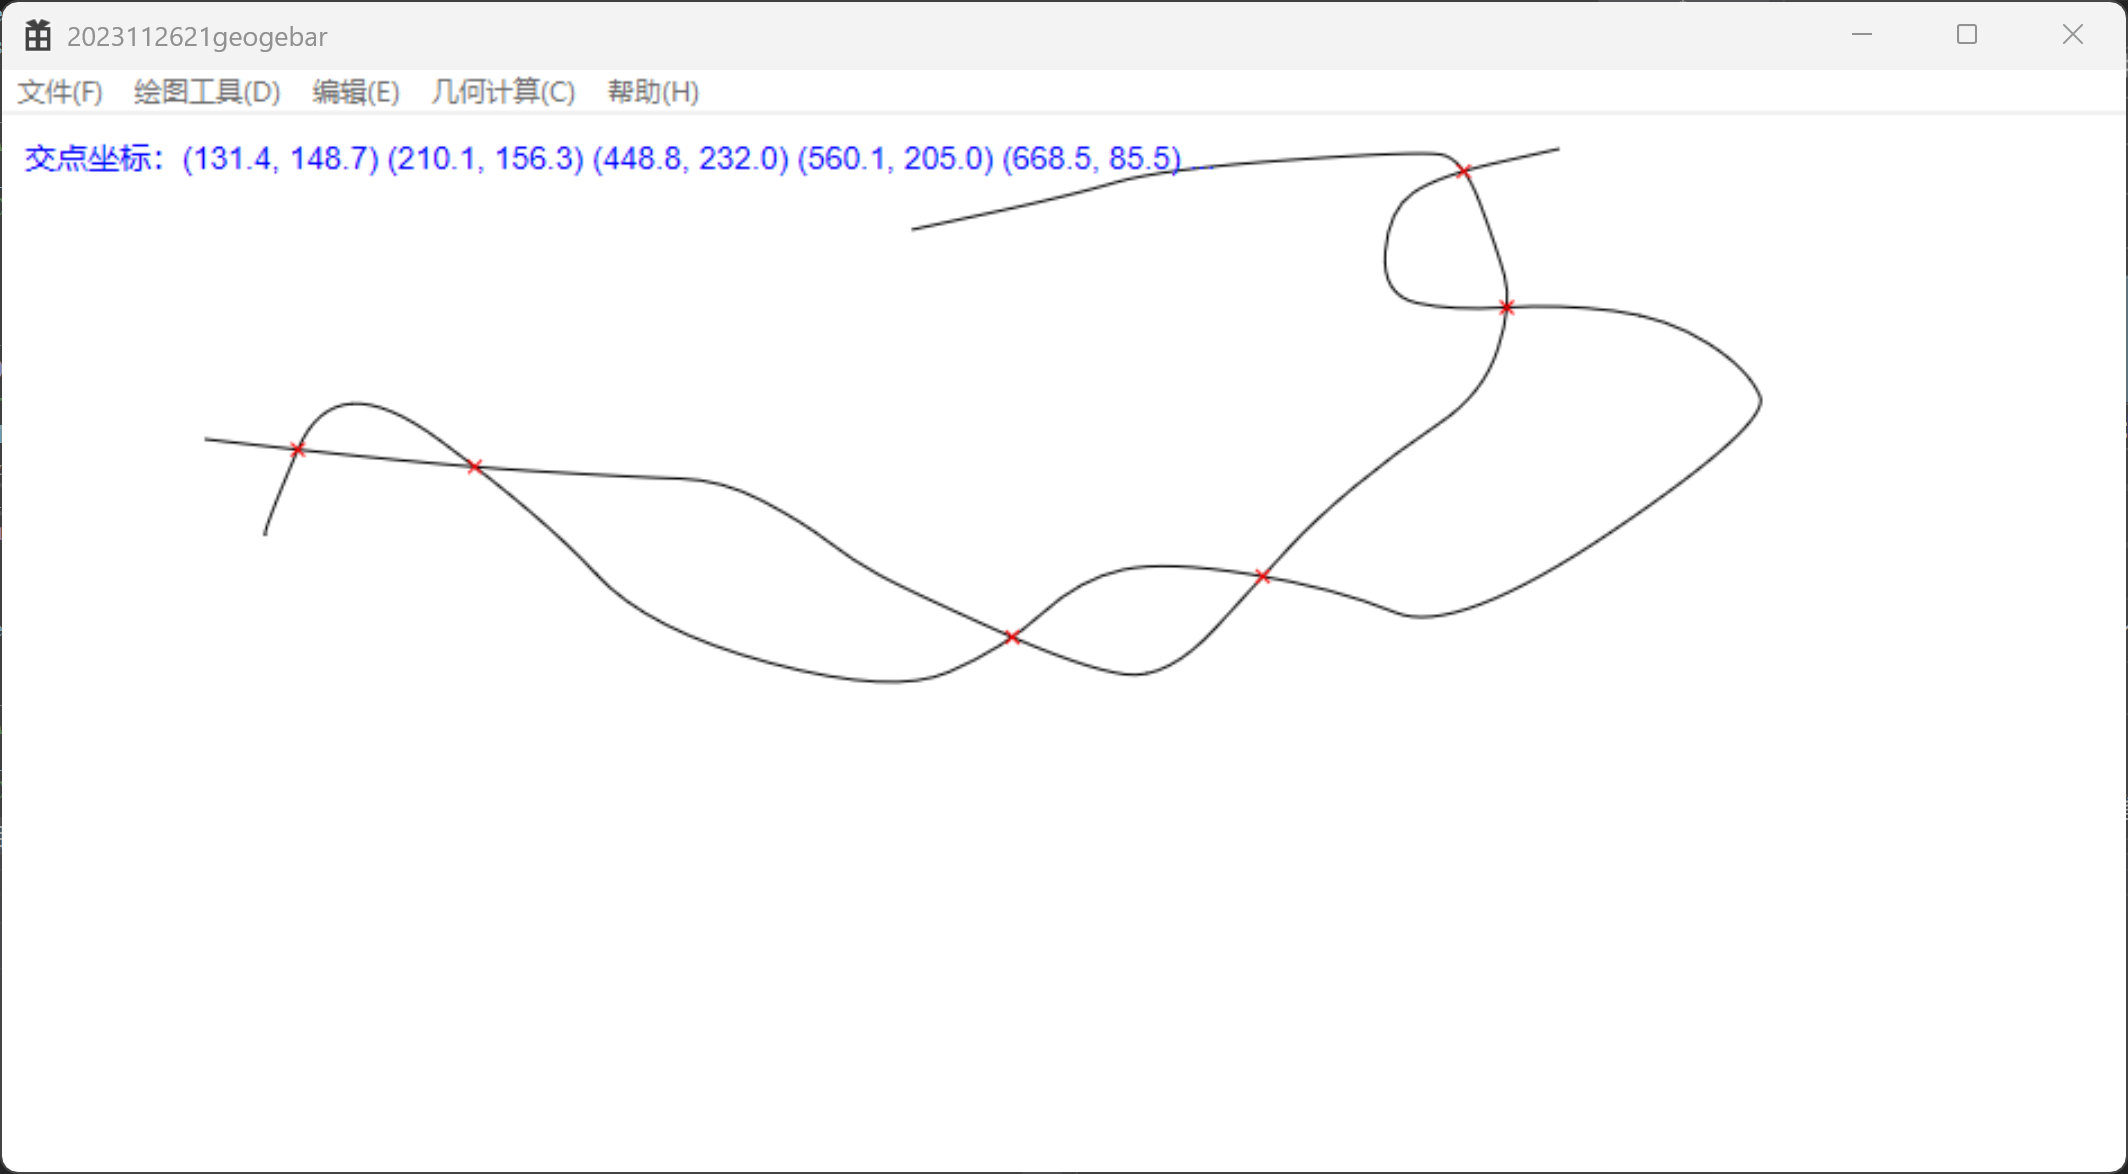
\includegraphics[width=0.92\textwidth]{images/qiujiao3.png}
	\caption{求交点示例}
\end{figure}

\textbf{2. 绘制垂线}
\begin{enumerate}
    \item 点击菜单"计算→垂线"
    \item 点击选择一条直线（用蓝色高亮显示）
    \item 在画布上点击一个点
    \item 系统自动绘制过该点的垂线（绿色虚线）
    \item 垂足位置用绿色圆点标记
    \item 显示垂足坐标信息
\end{enumerate}

% 在此处插入绘制垂线的截图
\begin{figure}[H]
	\centering
	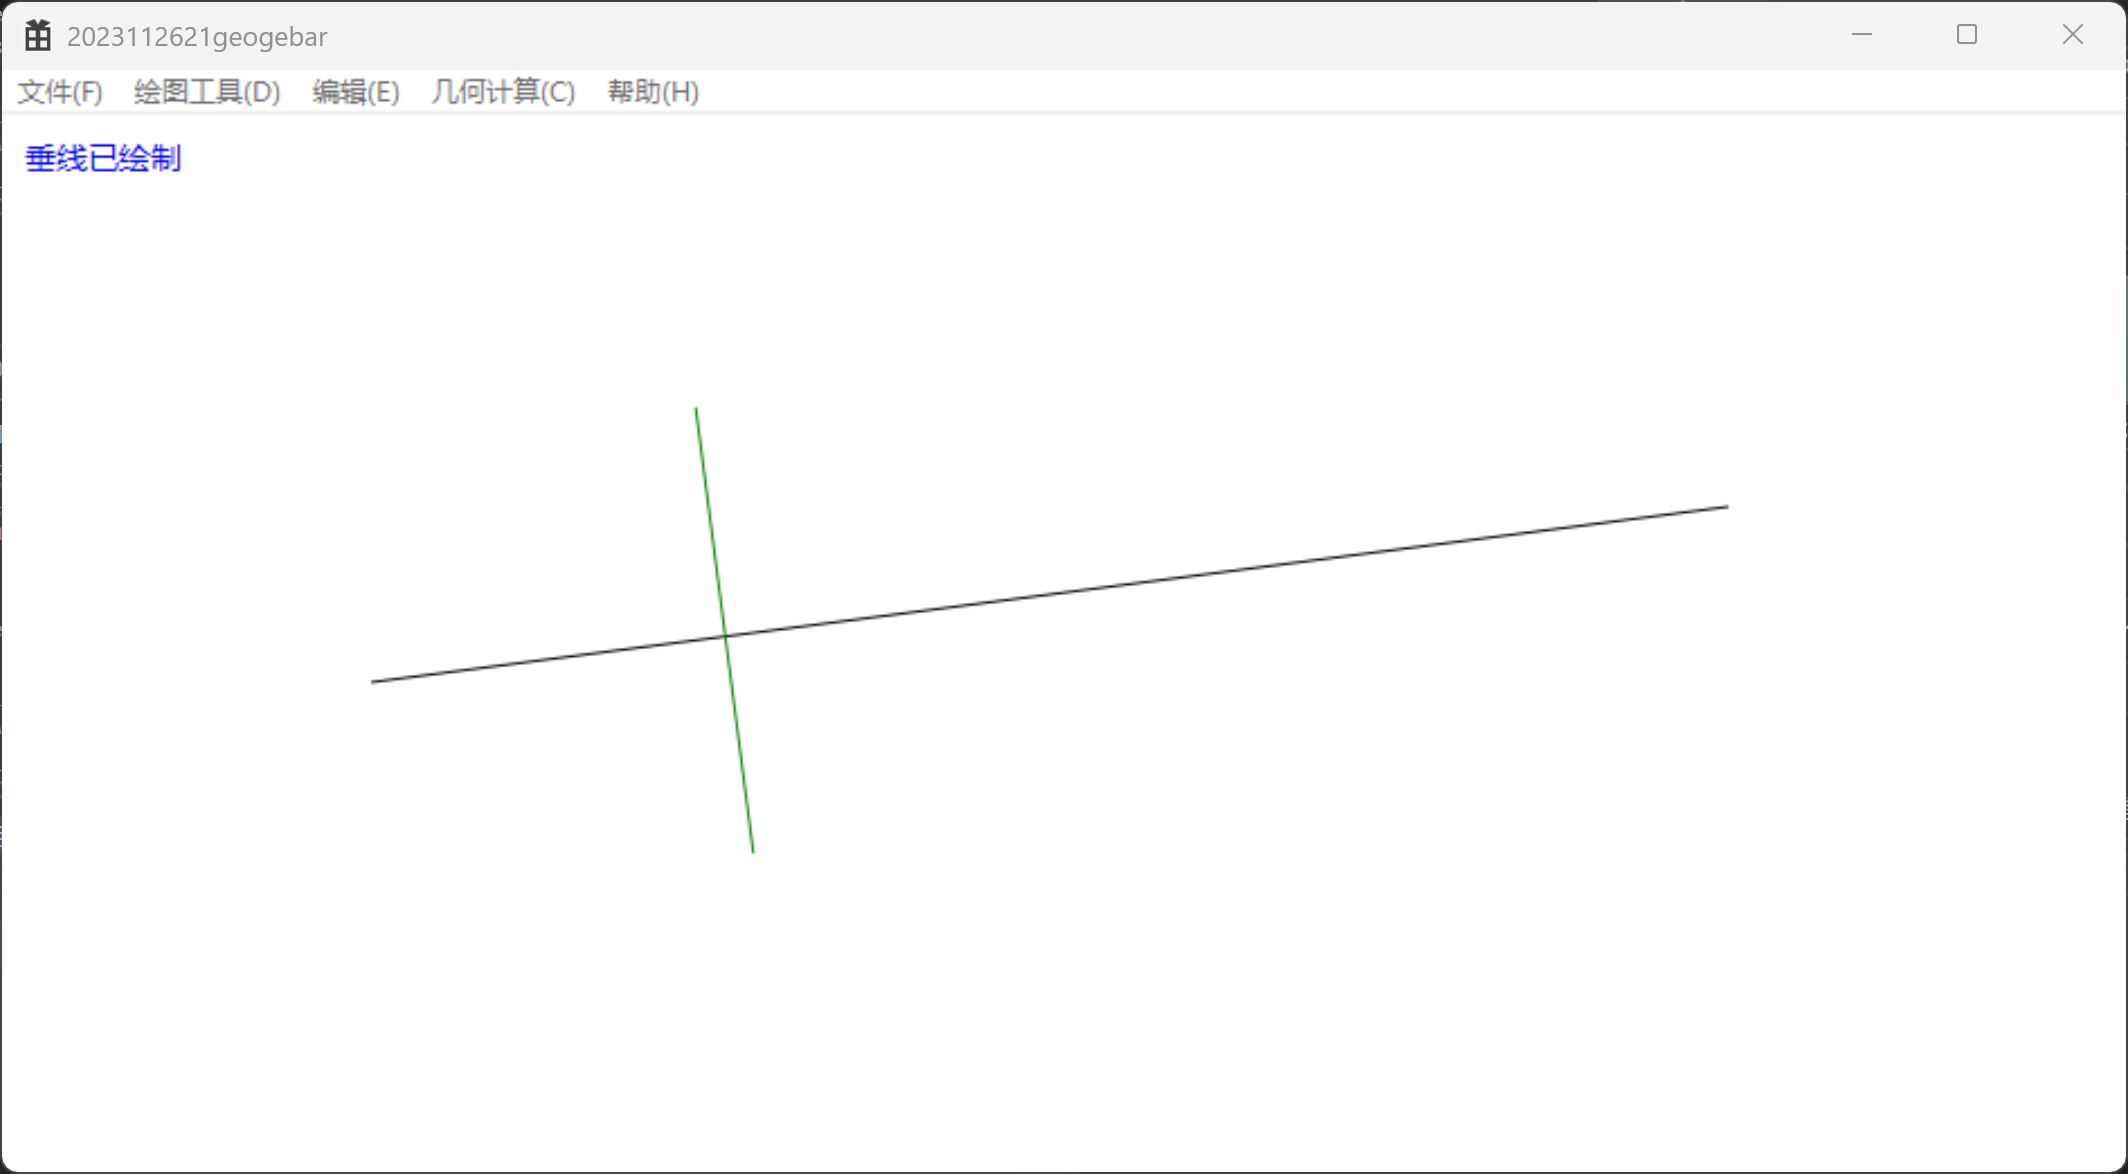
\includegraphics[width=0.92\textwidth]{images/chuixian.png}
	\caption{求垂线示例}
\end{figure}

\textbf{3. 显示圆心}
\begin{enumerate}
    \item 点击菜单"计算→圆心"
    \item 点击选择一个圆（用蓝色高亮显示）
    \item 系统在圆心位置绘制红色十字标记
    \item 显示圆心坐标、半径、周长和面积信息
\end{enumerate}

% 在此处插入显示圆心的截图
\begin{figure}[H]
	\centering
	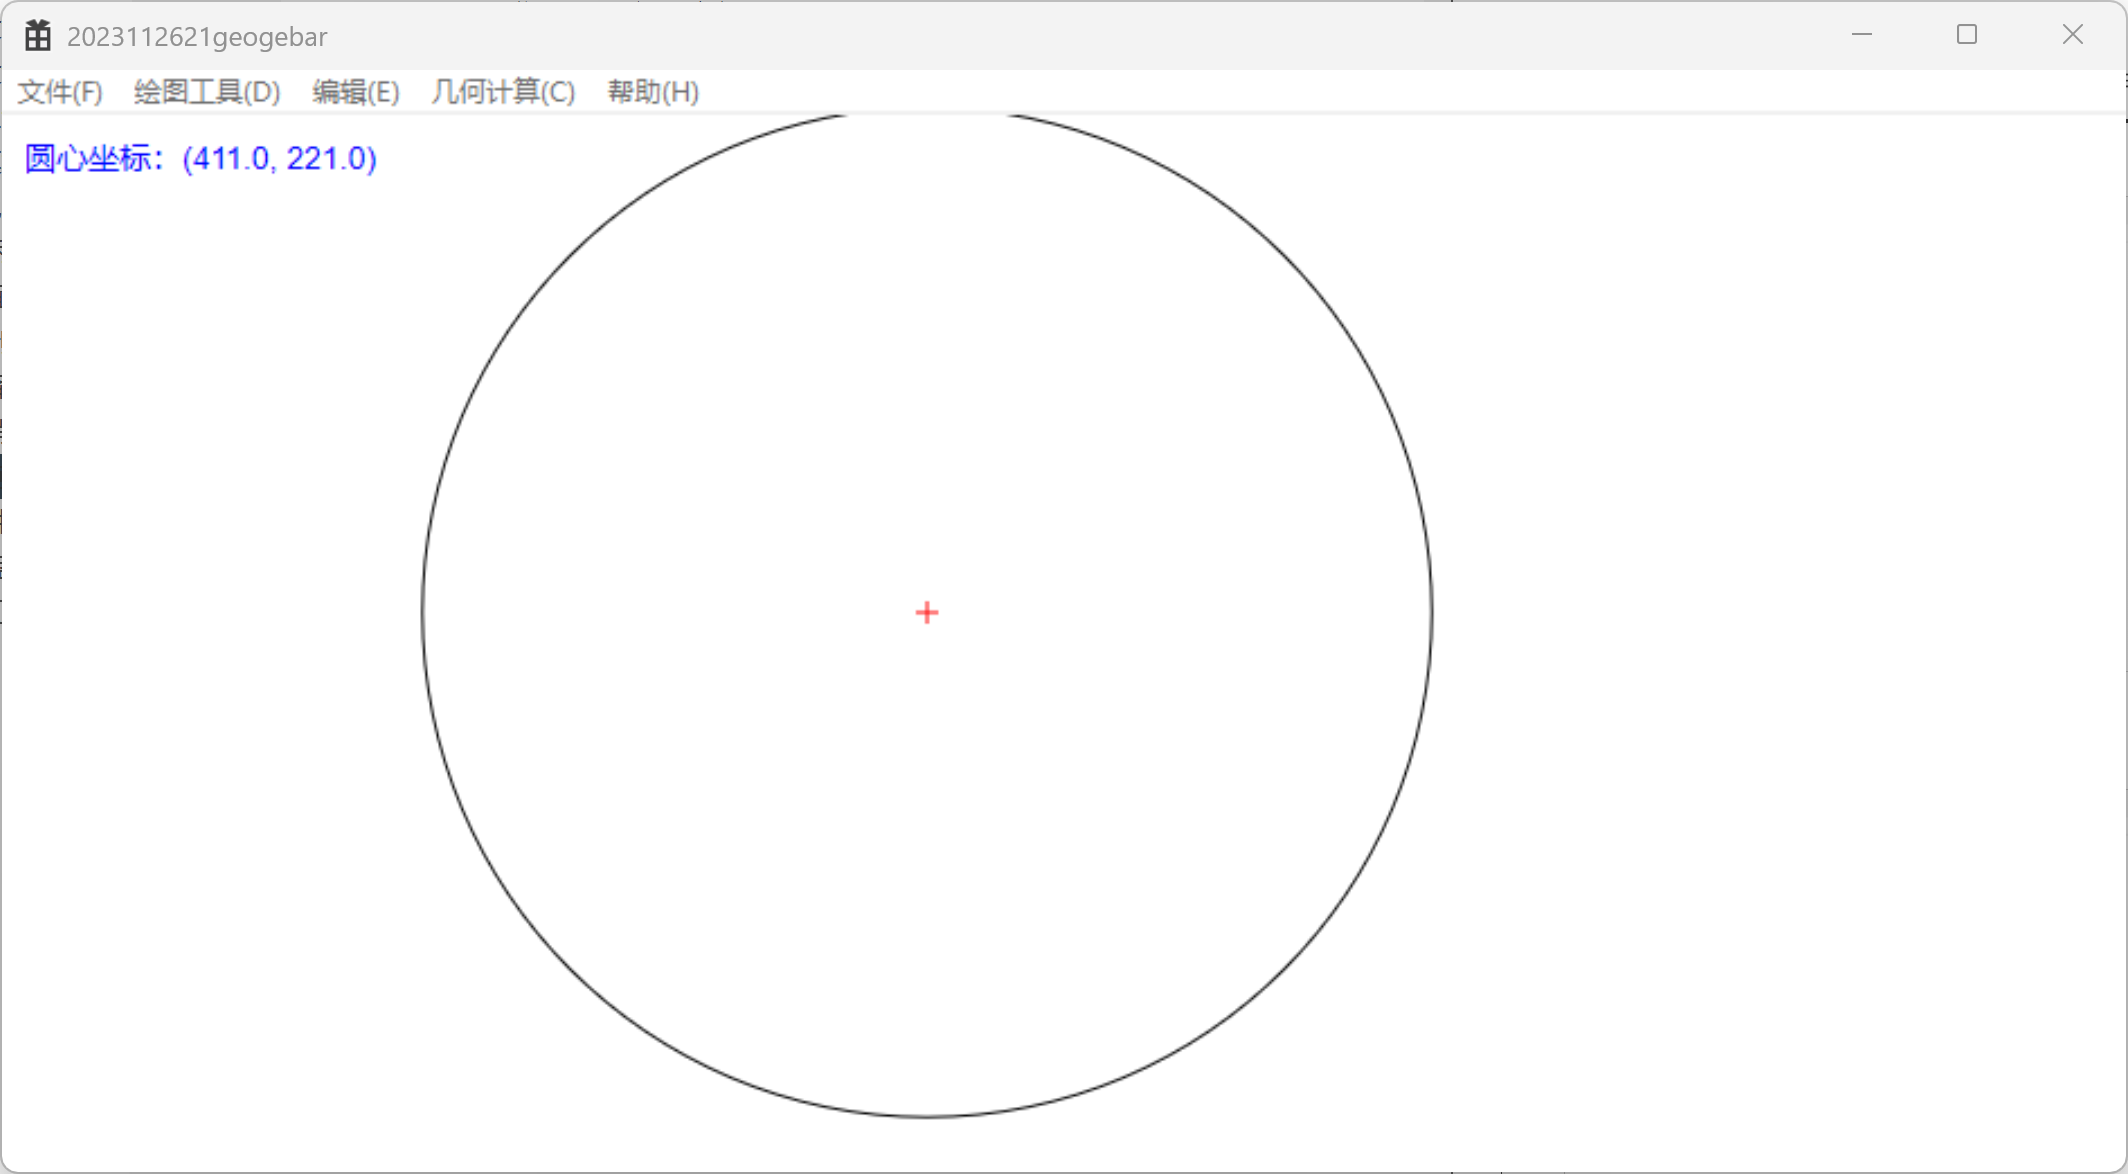
\includegraphics[width=0.92\textwidth]{images/yuanxin.png}
	\caption{求圆心示例}
\end{figure}

\textbf{4. 绘制切线}
\begin{enumerate}
    \item 点击菜单"计算→切线"
    \item 在画布上点击一个外部点
    \item 点击选择一个圆（用蓝色高亮显示）
    \item 系统自动绘制两条切线（紫色虚线）
    \item 两个切点用紫色圆点标记
    \item 显示切点坐标和切线长度信息
\end{enumerate}

\textbf{注意事项：}
\begin{itemize}
    \item 点必须在圆外才能绘制切线
    \item 点在圆上时只有一条切线
    \item 点在圆内时无法绘制切线
\end{itemize}

% 在此处插入绘制切线的截图
\begin{figure}[H]
	\centering
	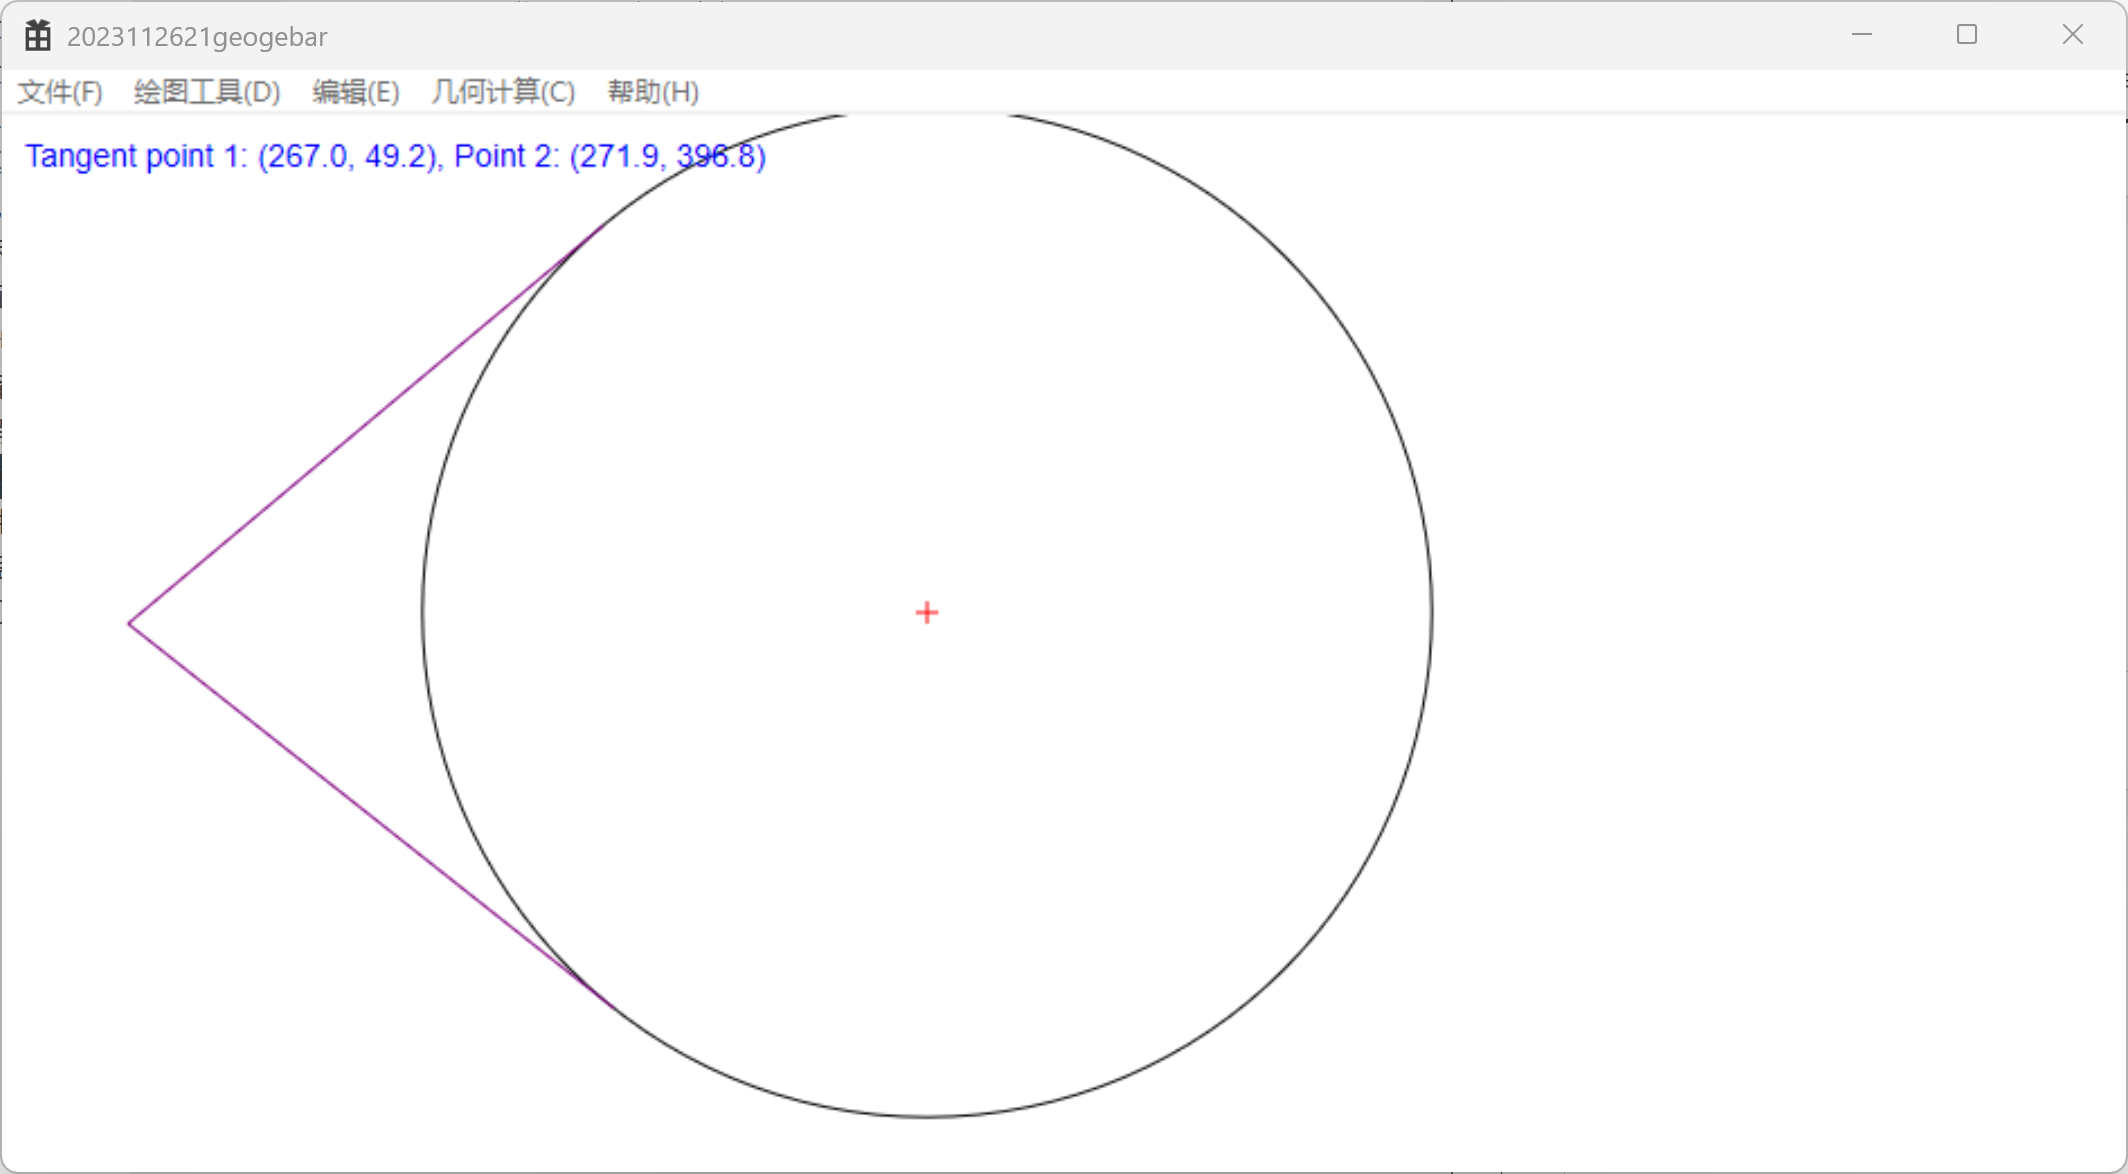
\includegraphics[width=0.92\textwidth]{images/qiexian.png}
	\caption{求切线示例}
\end{figure}
\end{tcolorbox}

\subsection{文件操作}

\begin{tcolorbox}
\textbf{1. 新建画布}
\begin{enumerate}
    \item 点击菜单"文件→新建"
    \item 如果当前有未保存的内容，系统会提示是否保存
    \item 确认后清空画布，开始新的绘图
\end{enumerate}

% 在此处插入新建画布的截图
\begin{figure}[H]
	\centering
	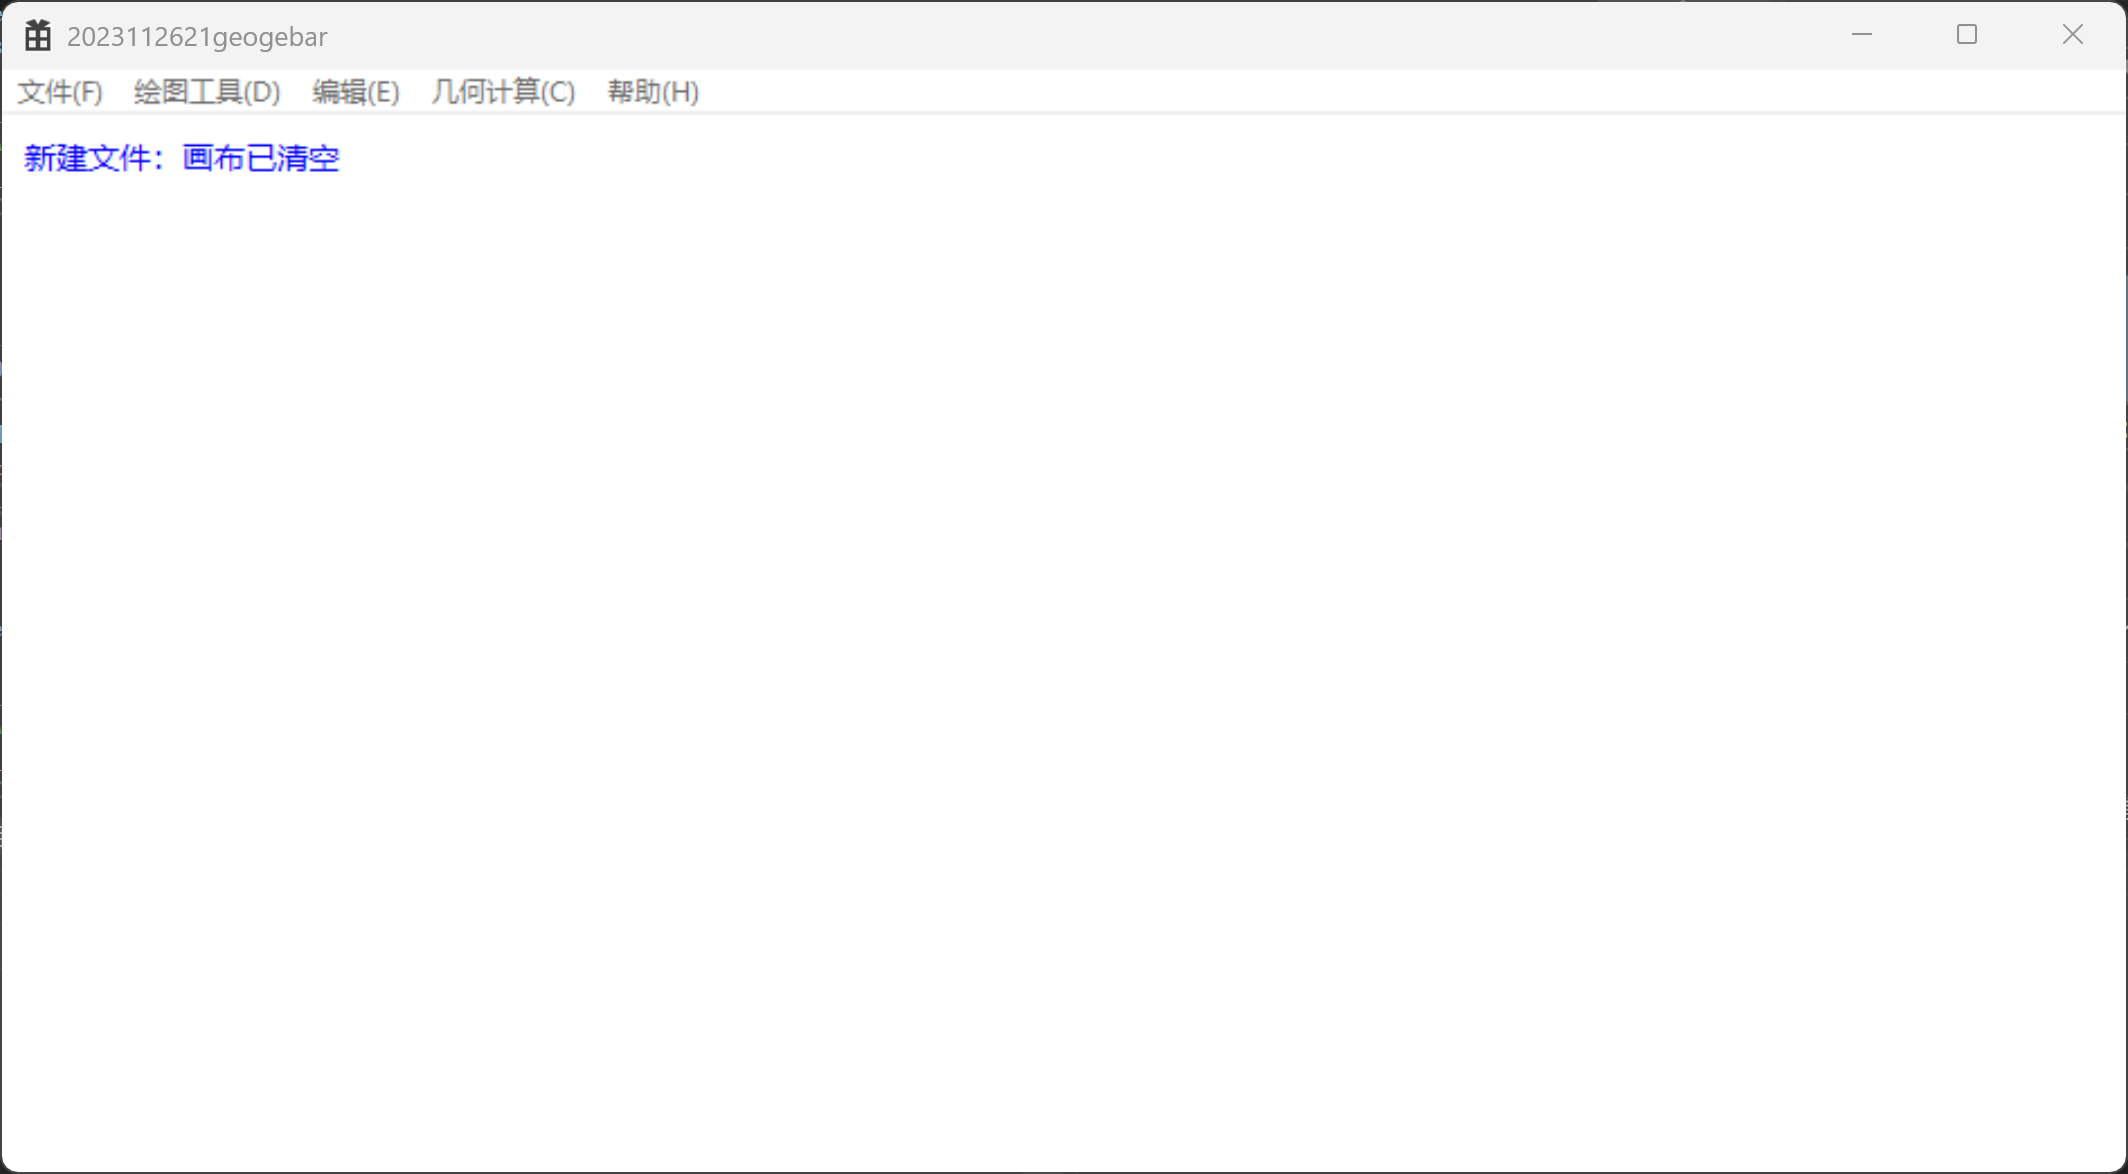
\includegraphics[width=0.92\textwidth]{images/xinjian.png}
	\caption{新建画布示例}
\end{figure}

\textbf{2. 保存文件}
\begin{enumerate}
    \item 点击菜单"文件→保存"
    \item 在弹出的保存对话框中选择保存位置
    \item 输入文件名（默认扩展名为.drw）
    \item 点击"保存"按钮
    \item 系统显示"文件保存成功"提示
\end{enumerate}

\textbf{文件格式说明：}
\begin{itemize}
    \item 文件扩展名：.drw
    \item 文件格式：纯文本格式
    \item 第一行：图形总数
    \item 后续每行：一个图形的序列化数据
\end{itemize}

% 在此处插入保存文件的截图
\begin{figure}[H]
	\centering
	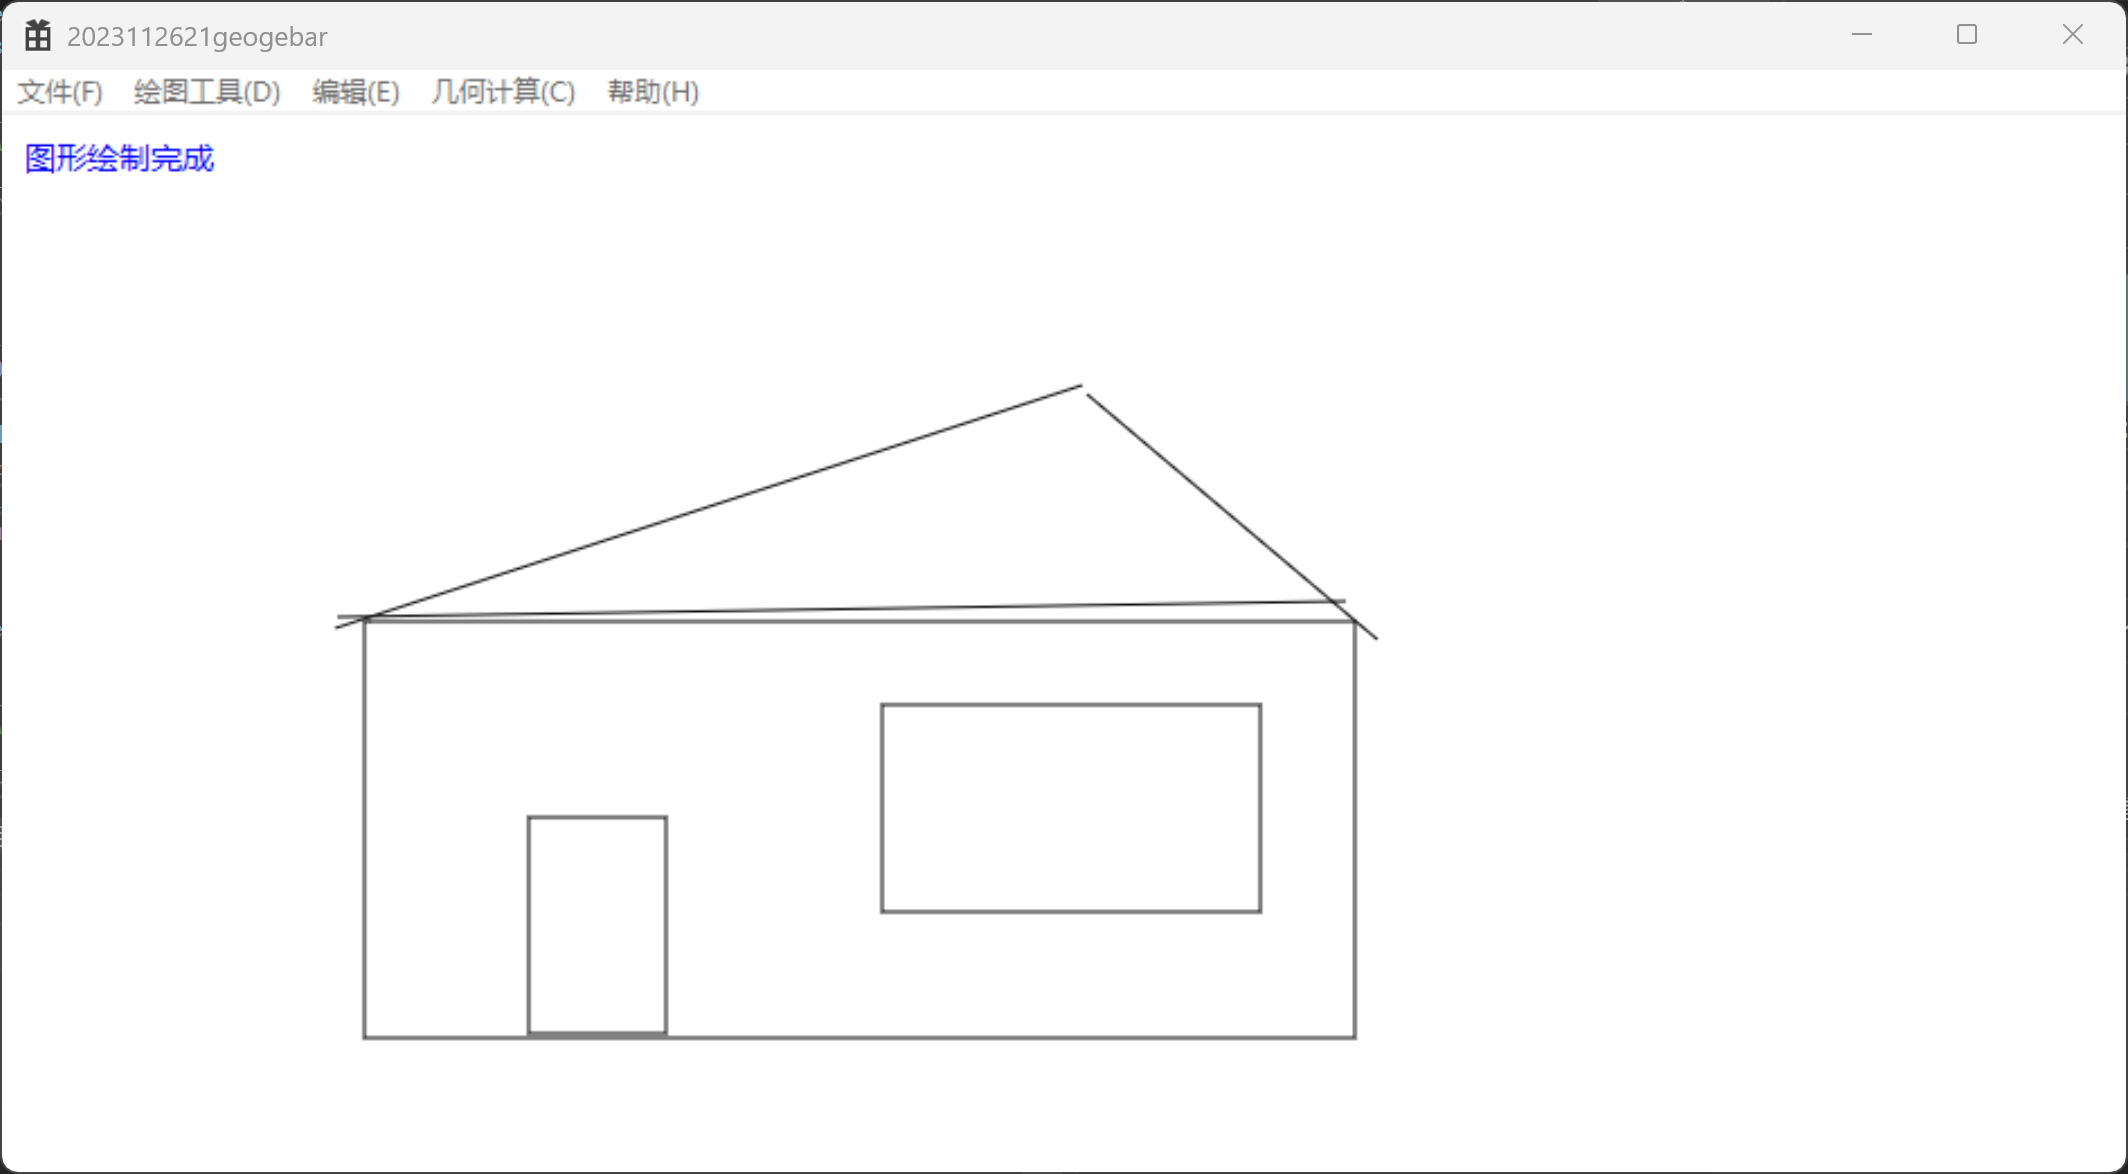
\includegraphics[width=0.92\textwidth]{images/bc1.png}
	\caption{保存示例}
\end{figure}
\begin{figure}[H]
	\centering
	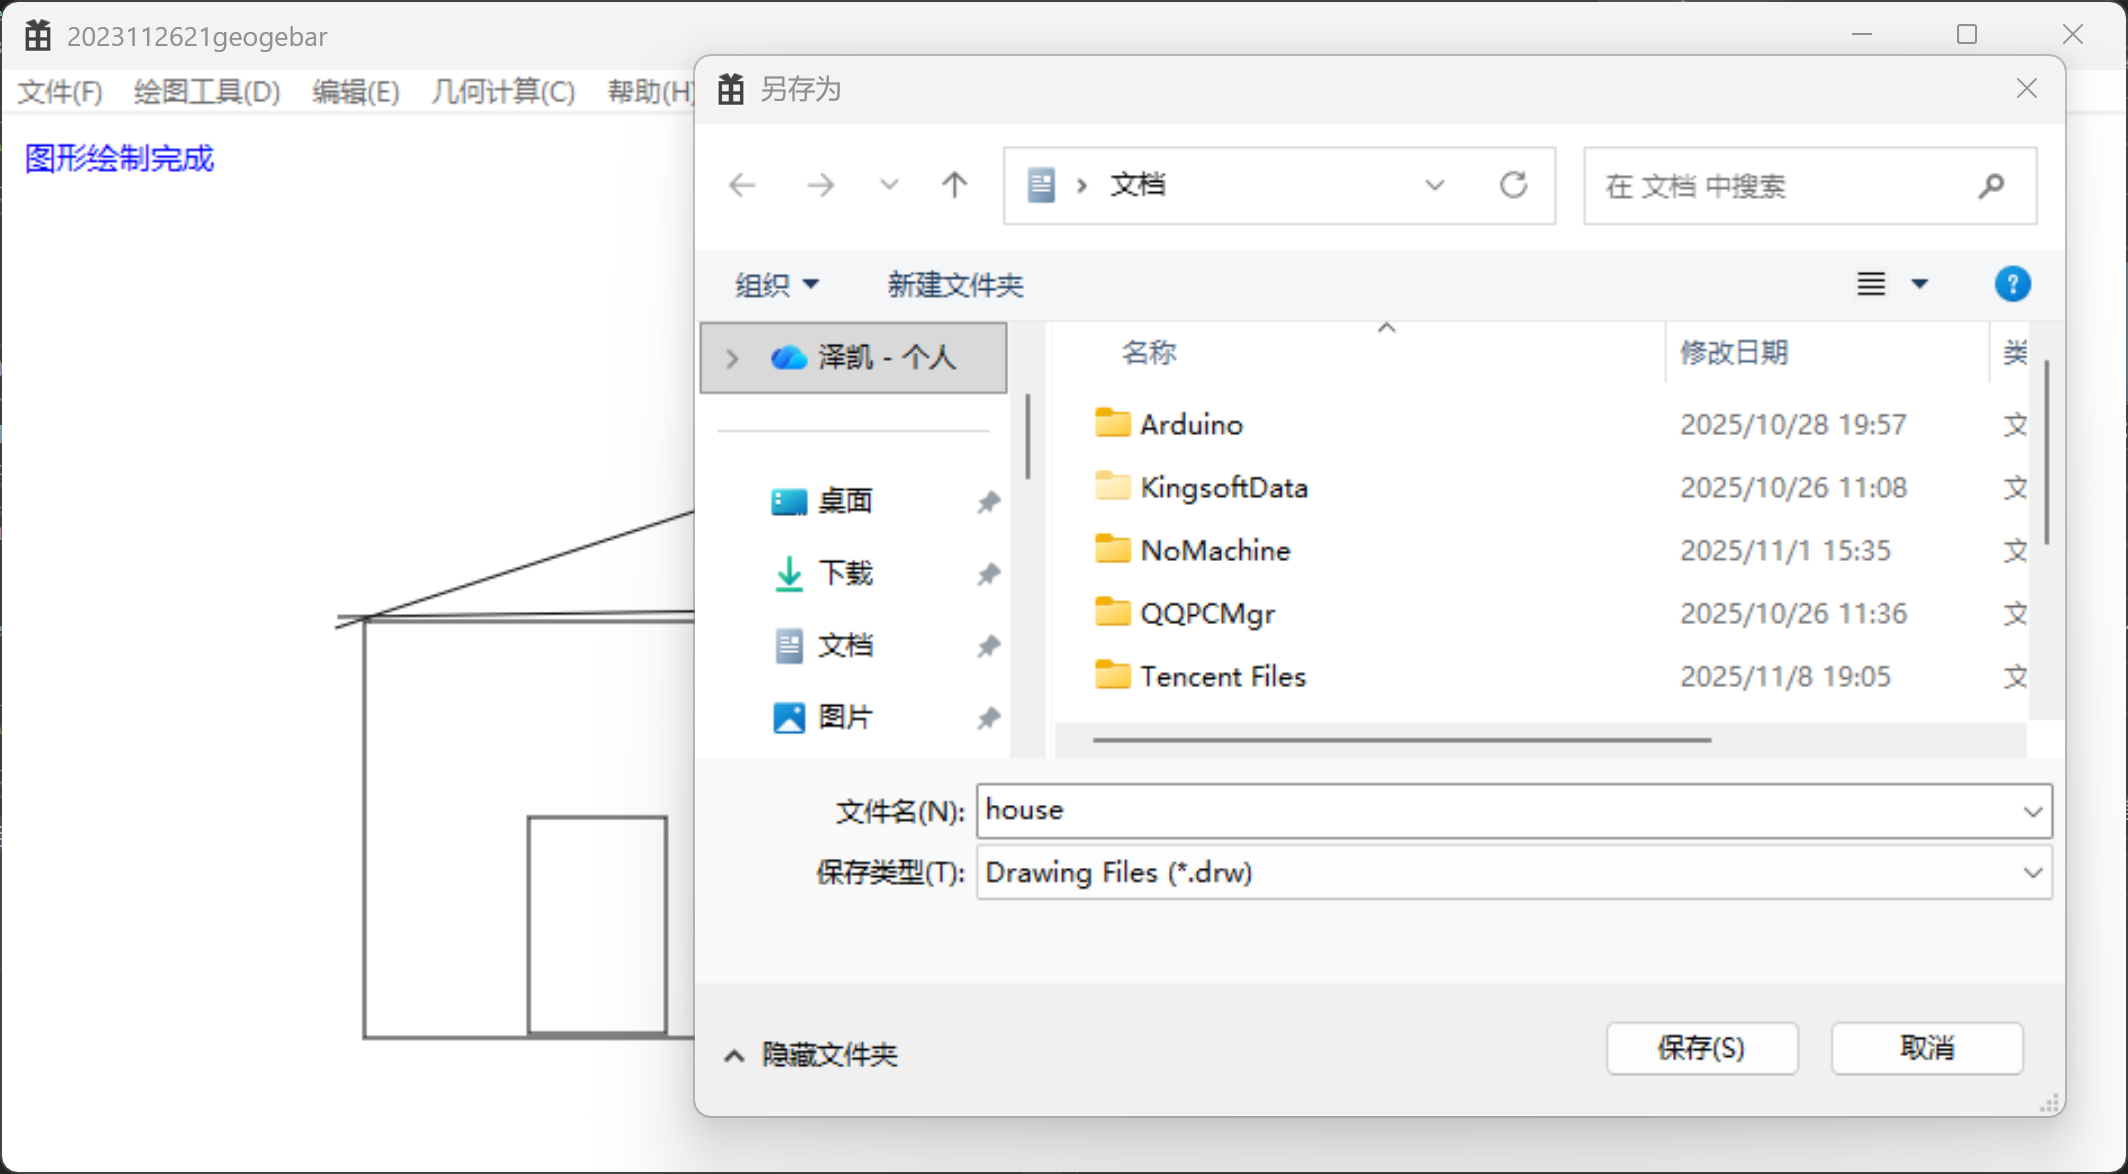
\includegraphics[width=0.92\textwidth]{images/bc2.png}
	\caption{保存示例}
\end{figure}
\begin{figure}[H]
	\centering
	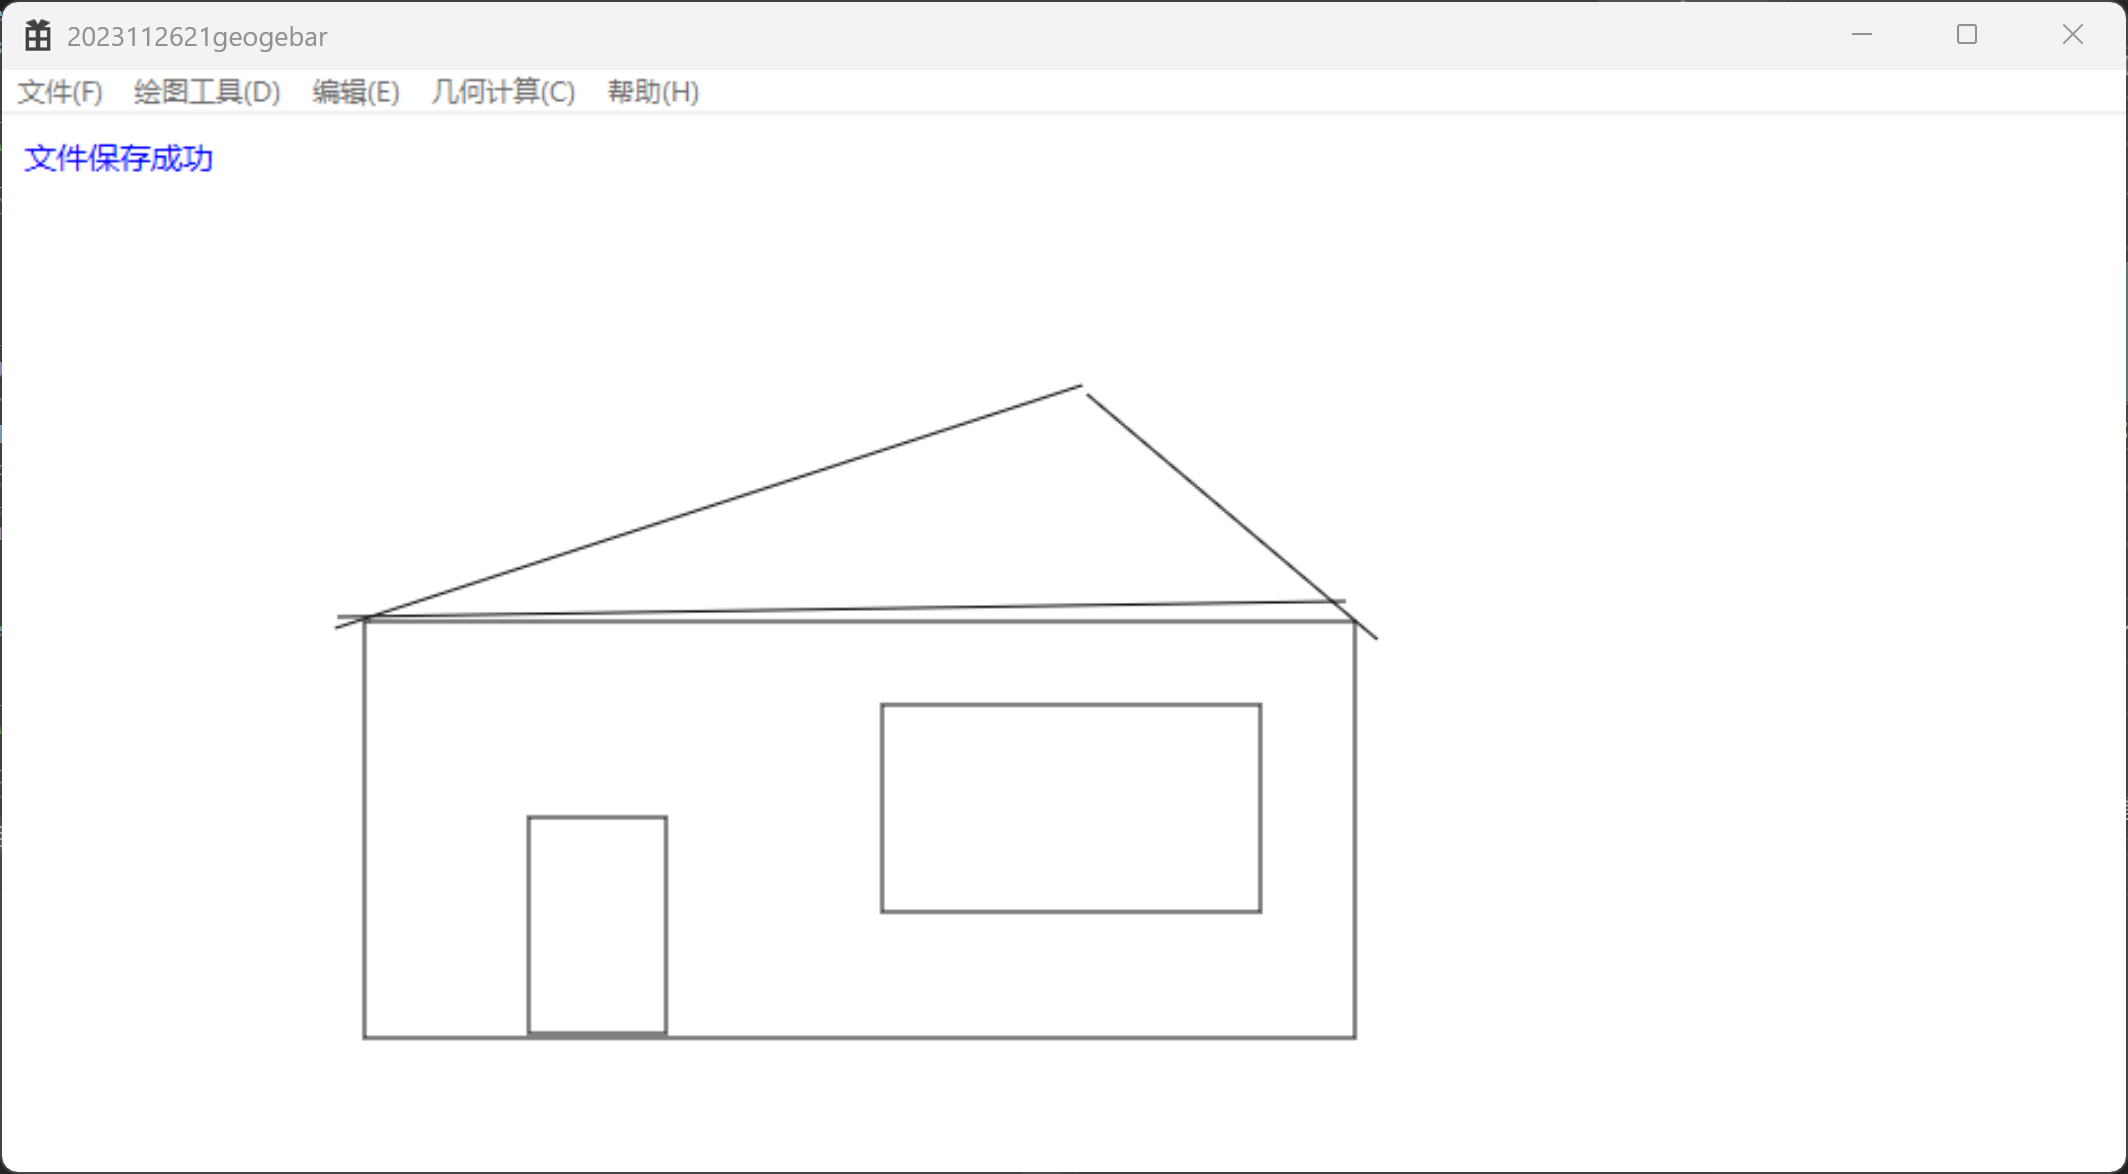
\includegraphics[width=0.92\textwidth]{images/bc3.png}
	\caption{保存示例}
\end{figure}

\textbf{3. 打开文件}
\begin{enumerate}
    \item 点击菜单"文件→打开"
    \item 在弹出的打开对话框中选择.drw文件
    \item 点击"打开"按钮
    \item 系统清空当前画布并加载文件中的图形
    \item 显示"文件加载成功"提示
\end{enumerate}

% 在此处插入打开文件的截图
\begin{figure}[H]
	\centering
	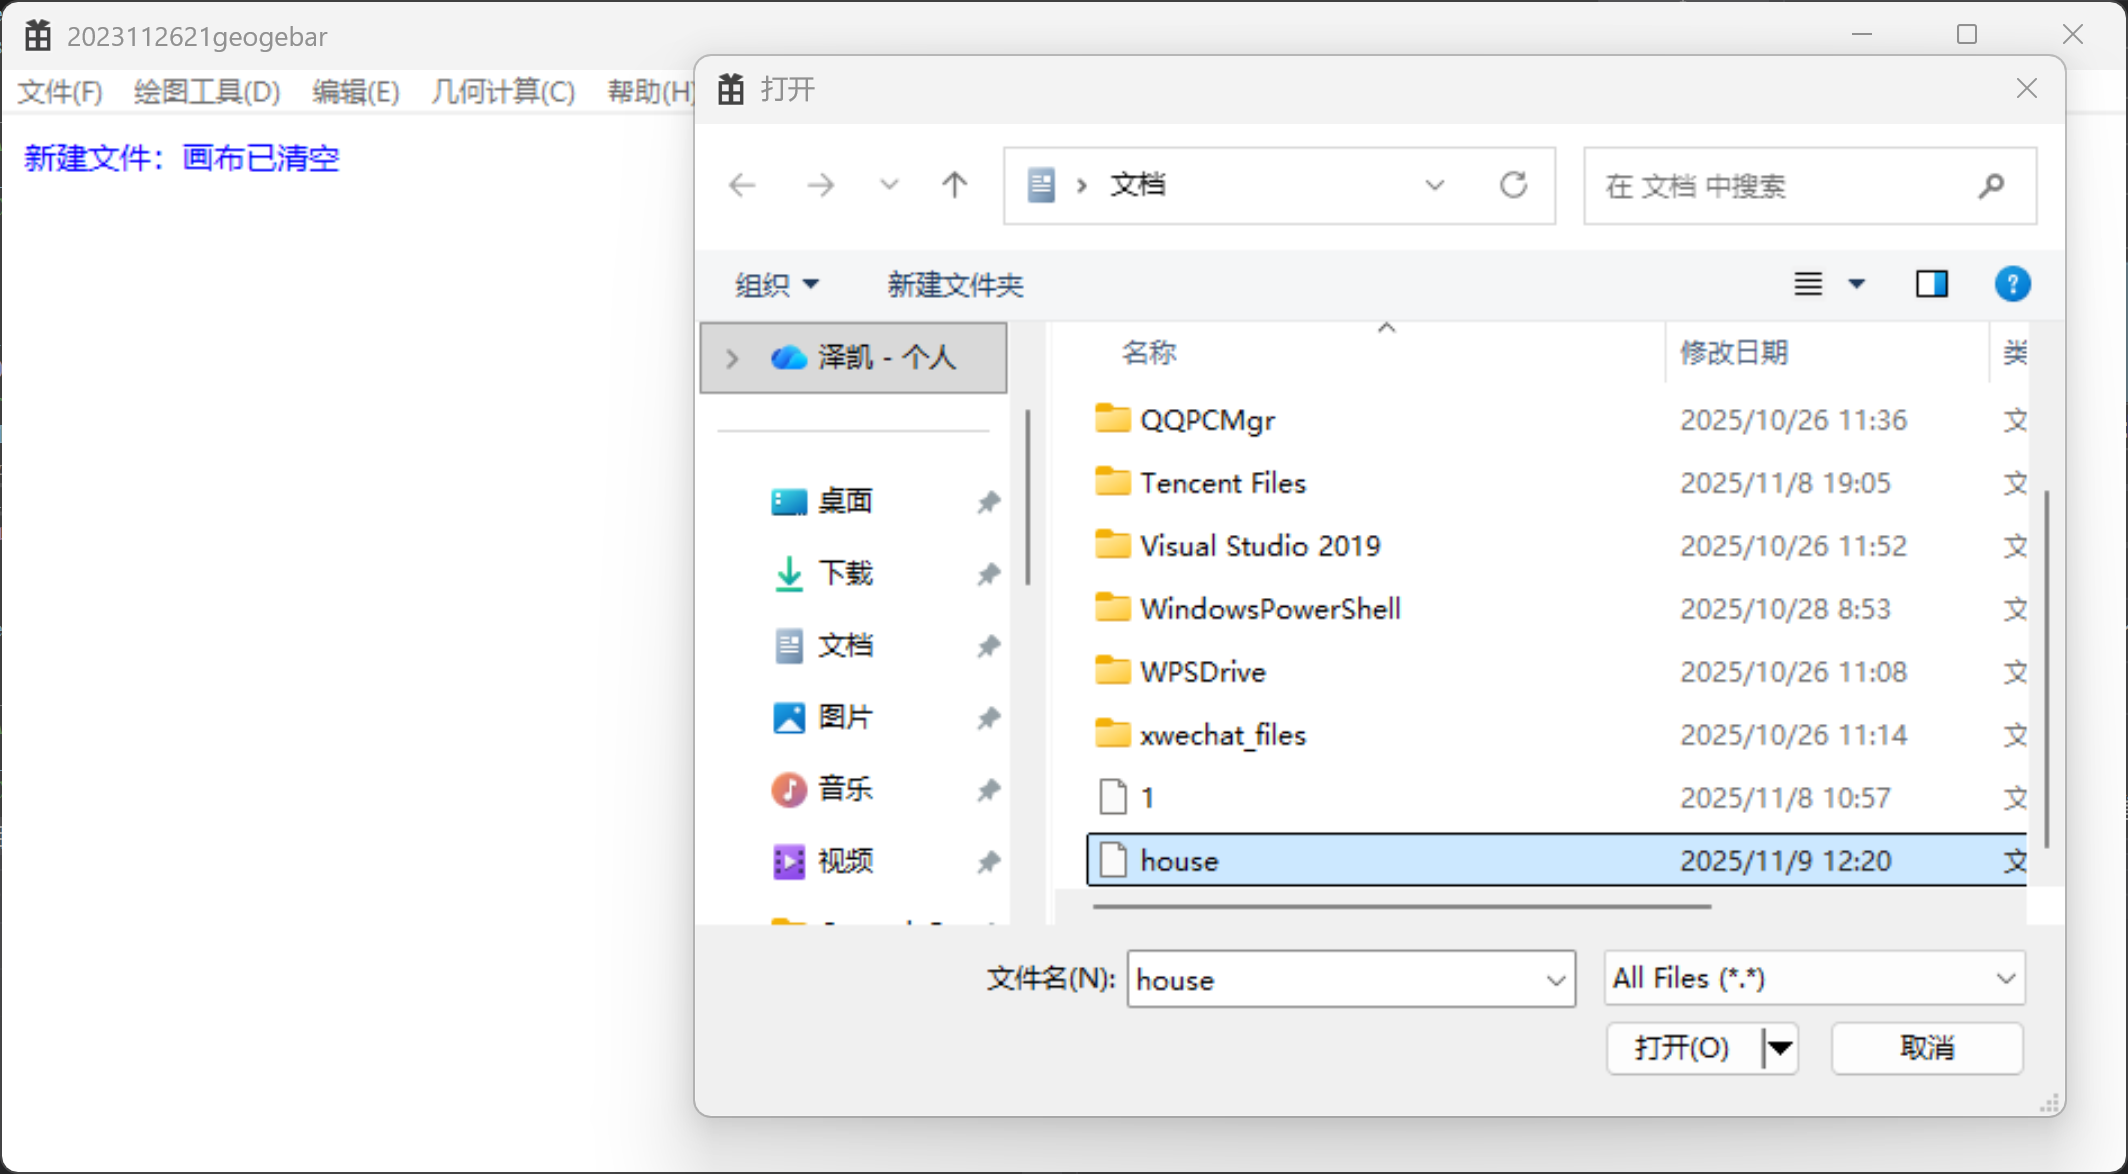
\includegraphics[width=0.92\textwidth]{images/jz1.png}
	\caption{加载示例}
\end{figure}
\begin{figure}[H]
	\centering
	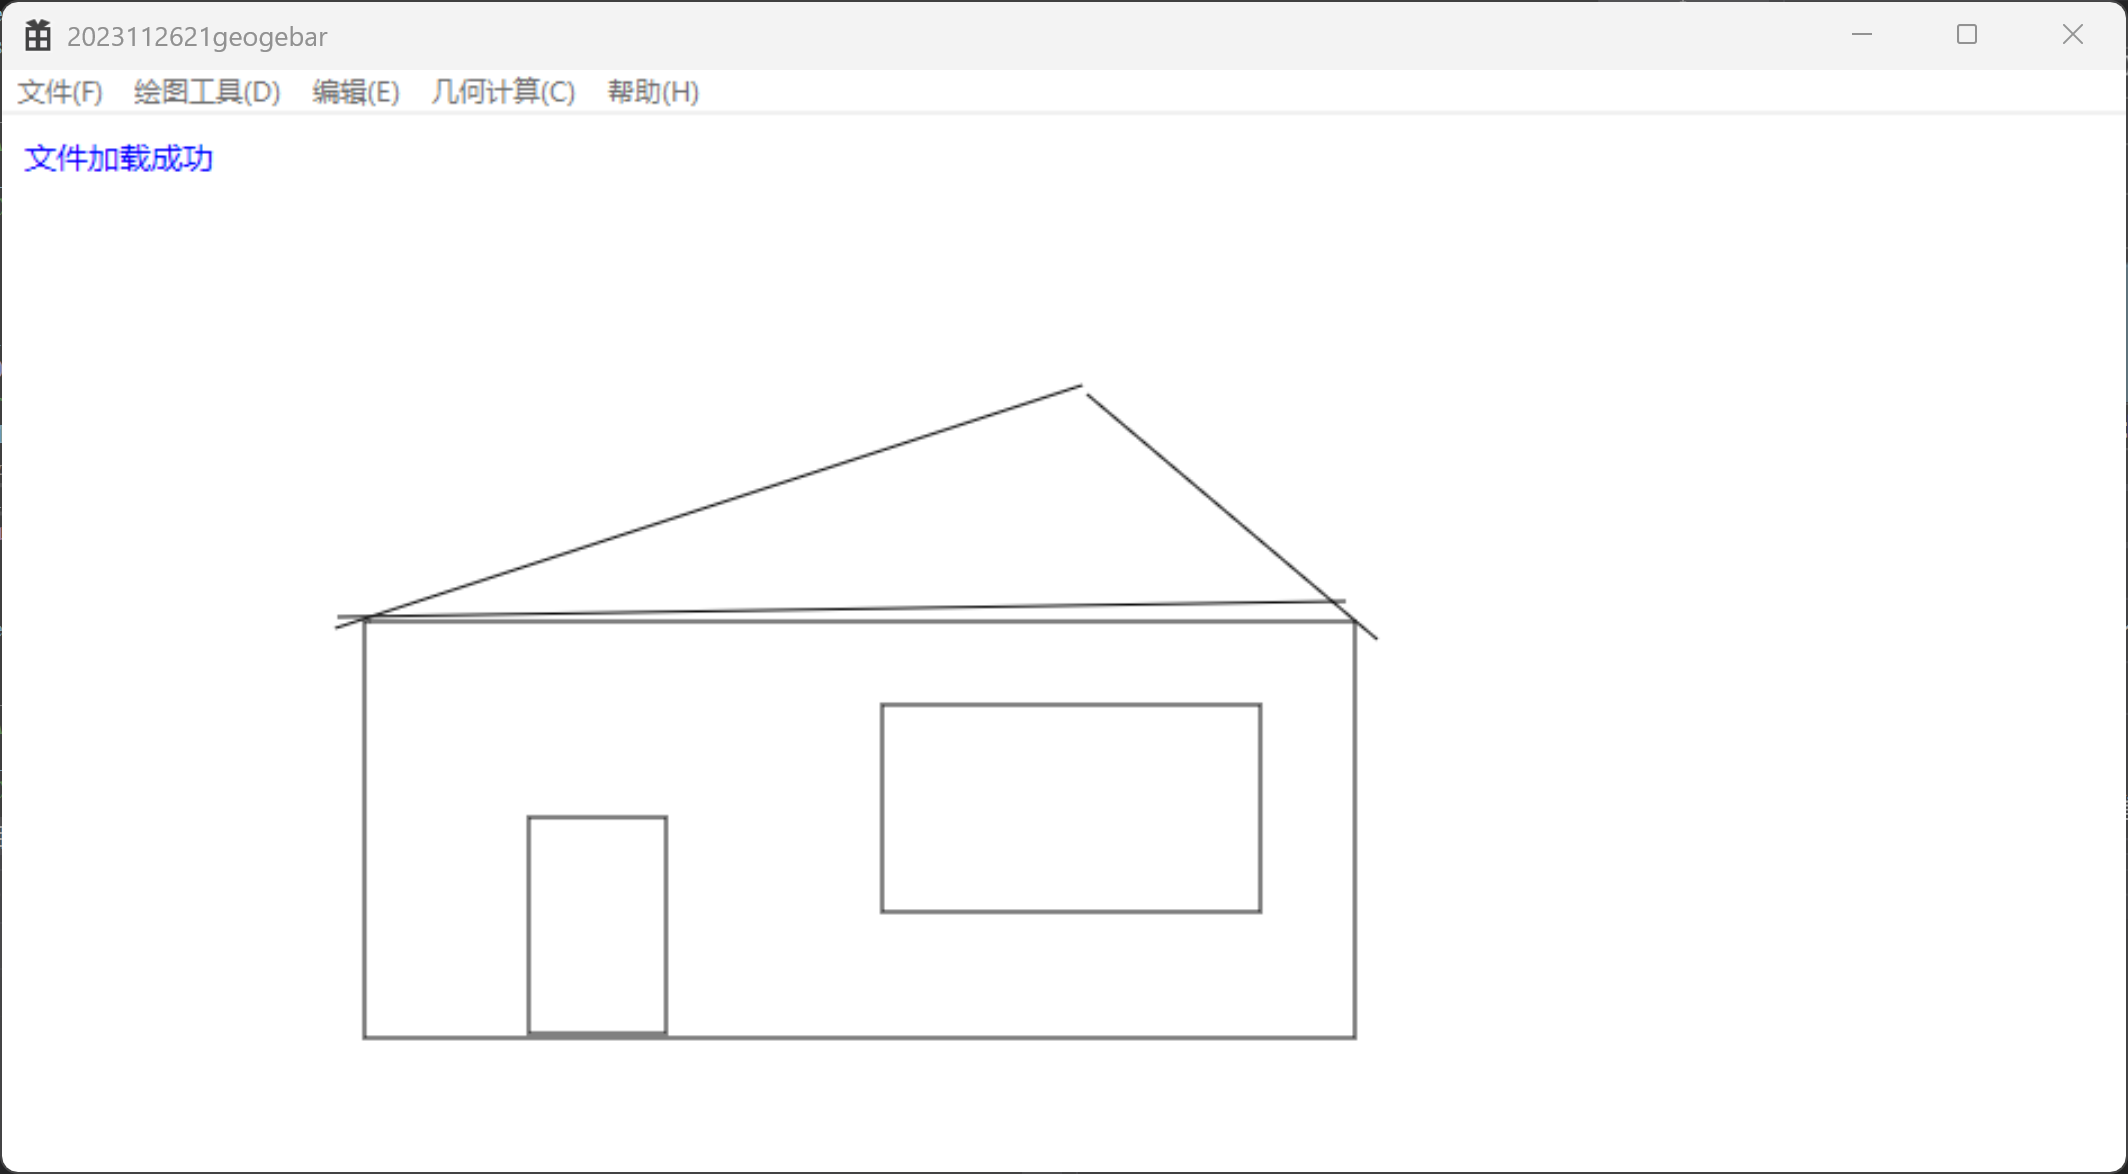
\includegraphics[width=0.92\textwidth]{images/jz2.png}
	\caption{加载示例}
\end{figure}

\textbf{4. 退出程序}
\begin{enumerate}
    \item 点击菜单"文件→退出"或点击窗口关闭按钮
    \item 如果有未保存的内容，系统会提示是否保存
    \item 确认后程序退出
\end{enumerate}
\end{tcolorbox}

\section{实验总结}

\begin{tcolorbox}
通过本次实验，我成功设计并实现了一个功能完整的简单绘图软件，主要收获如下：

\begin{enumerate}
    \item \textbf{系统设计能力}：学会了如何设计一个完整的图形交互系统，包括数据结构设计、模块划分、接口定义等。掌握了面向对象的设计方法，通过继承和多态实现了灵活可扩展的图形框架。
    
    \item \textbf{图形编程技术}：深入掌握了Direct2D的高级应用，包括渲染目标管理、画刷样式设置、虚线绘制等技术。学会了如何实现图形的HitTest、变换操作等核心功能。
    
    \item \textbf{事件处理机制}：理解了Windows消息机制，掌握了鼠标事件（点击、移动、滚轮）的处理方法。学会了如何设计状态机来管理不同的操作模式（绘制、选择、编辑等）。
    
    \item \textbf{状态管理技术}：实现了完整的撤销/重做功能，掌握了使用双栈结构管理历史状态的方法。通过序列化/反序列化实现了图形的深拷贝，理解了状态独立性的重要性。
    
    \item \textbf{交互设计优化}：改进了旋转和缩放的交互方式，使用鼠标滚轮配合实时预览和取消功能，大大提升了用户体验。学会了如何设计直观、友好的用户交互界面。
    
    \item \textbf{几何算法应用}：实现了多种几何计算算法，包括点到线距离、直线求交、圆-圆求交、切线计算等。将数学知识应用到实际编程中，提高了算法实现能力。
    
    \item \textbf{文件格式设计}：学会了如何设计简单的文件格式，实现了图形数据的序列化和反序列化。理解了数据持久化的基本原理。
    
    \item \textbf{调试与测试}：通过大量的测试和调试，提高了发现和解决问题的能力。学会了如何系统地测试软件的各项功能。
\end{enumerate}

\textbf{遇到的主要问题及解决方案：}

\begin{itemize}
    \item \textbf{问题1}：图形选择的HitTest精度问题。\textbf{解决}：为不同类型的图形设计了不同的HitTest算法，并设置了合理的容差值。
    
    \item \textbf{问题2}：图形旋转时的中心点计算。\textbf{解决}：为每种图形实现了GetCenter()方法，根据图形类型计算几何中心。
    
    \item \textbf{问题3}：虚线绘制的实现。\textbf{解决}：使用Direct2D的StrokeStyle功能，创建虚线样式并应用到选中图形的绘制。
    
    \item \textbf{问题4}：文件格式的设计。\textbf{解决}：采用简单的文本格式，每种图形一行，便于调试和扩展。
    
    \item \textbf{问题5}：旋转和缩放的交互体验。\textbf{解决}：改用鼠标滚轮进行调整，配合实时预览和取消功能，提供更好的用户体验。用户可以在确认前看到效果，不满意可以右键取消。
    
    \item \textbf{问题6}：撤销/重做的深拷贝问题。\textbf{解决}：通过序列化和反序列化实现图形的深拷贝，确保状态独立性。每次保存状态时都创建完全独立的图形副本。
\end{itemize}

本实验不仅巩固了图形编程的基础知识，更重要的是培养了完整系统的设计与实现能力。通过实践，深刻理解了软件工程的基本原则，为后续更复杂的图形应用开发奠定了坚实的基础。
\end{tcolorbox}

\end{document}